\graphicspath{{Dissertation/images/chapt3/}}

\chapter{Экстремальные яркостные температуры в обзоре активных ядер галактик} \label{chapt3}

\section{Яркостная температура}

\section{Обзор активных ядер галактик в проекте <<РадиоАстрон>>}


\section{RELATIVISTIC JETS IN THE RADIO REFERENCE FRAME IMAGE DATABASE. II. BLAZAR JET
ACCELERATIONS FROM THE FIRST 10 YEARS OF DATA (1994--2003)}
% \section{Измерение доплеровского усиления с помощью кинематики релятивистских струй}

\subsection{Введение}

Объемный отток вещества при высоких факторах Лоренца в коллимированных релятивистских струях
является хорошо известным свойством мощных блазаров. Такие высокие факторы Лоренца можно
непосредственно наблюдать по видимому движению высокоскоростных компонентов струи на изображениях,
построенных с помощью  интерферометрии со сверхдлинными базами (РСДБ) \cite{Lister_2009b}, и они
также необходимы для объяснения спектрального распределения энергии блазаров \cite{Hartman_2001},
переменности гамма-излучения \cite{Dondi_1995} и высокой яркостной температуры радио-ядра
\cite{Tingay_2001}. Эти релятивистские джеты должны ускорятся на масштабах расстояний от примерно
$10^3$ гравитационных радиусов от центральной черной дыры и до парсеков, где они непосредственно
наблюдаются с помощью РСДБ \cite{Sikora_2005,Vlahakis_2004}. Хотя наблюдения за потоками с высоким
фактором Лоренца хорошо установлены, теоретический механизм, с помощью которого эти потоки
ускоряются, и масштаб длины, на котором они работают, до конца не поняты.

В общем контексте ускорения магнитной струи в блазарах \cite{Sikora_2005} энергия потока начинается
как магнитная энергия, или поток вектора Пойнтинга, который затем преобразуется в объемную
кинетическую энергию во время фазы ускорения и, наконец, в кинетическую энергию частиц при ударах,
которая затем может излучиться. Магнитное ускорение было исследовано с помощью релятивистского
магнитогидродинамического моделирования (например \cite{McKinney_2006}; также см.
\cite{Komissarov_2011,Konigl_2010} для краткого описания теории магнитного ускорения релятивистских
струй).

Остается рассмотреть ряд деталей в этой общей структуре: например, создается ли струя в устойчивом
состоянии или ускорение является импульсным \cite{Granot_2011,Lyutikov_2010}, и
завершается ли ускорение на масштабах, наблюдаемых на РСДБ, или все еще происходит на
парсековых масштабах. В \cite{Vlahakis_2004} утверждается, что магнитное ускорение может
продолжать действовать в масштабах парсеков, и они интерпретировали два конкретных наблюдаемых
события ускорения в NGC\,6251 и 3C\,345 как свидетельство этого <<магнитного движения>> в
парсековых масштабах, но во времена той статьи было ещё недостаточно РСДБ наблюдений для
решения вопроса о том, является ли ускорение на масштабах парсеков общим свойством струй блазаров
на больших выборках. Даже если явление ускорения в масштабе парсек считается обычным явлением, это
не обязательно доказывает прямое наблюдение преобразования потока Пойнтинга в кинетическую энергию,
поскольку также могут быть гидродинамические механизмы для создания ускорений в джетах с
доминированием вещества \cite{Daly_1988,Kadler_2008}, или наблюдения могут
показывать увеличение факторов Лоренца структур в подстилающем потоке.

Прямые наблюдения внутреннего ускорения с помощью РСДБ картографирования затруднены. Точные
измерения положения компонентов на многих эпохах необходимы для надежного измерения второй
производной на графике положения от времени. Для отдельных компонентов струи кажущаяся скорость
определяется по известной формуле:
\begin{equation}
\label{speedeqn}
 \beta_\text{app} = \frac{\beta \sin\theta}{1 - \beta \cos\theta}\,,
\end{equation}
где $\beta c$~"--- собственная скорость, а $\theta$~"--- угол движения к лучу зрения. При
наблюдении в одном компоненте изменения кажущейся скорости могут быть вызваны либо изменением
собственной скорости, либо угла обзора. Наблюдения за многими явно ускоряющимися компонентами
необходимы для статистического различия между этими двумя случаями. На практике, наблюдения за
многими источниками во многие эпохи, насчитывающие тысячи изображений РСДБ, необходимы для измерения
вариаций собственных скоростей. В то время как наблюдения за отдельными кажущимися ускорениями
компонентов (например, \cite{Unwin_1997,Homan_2003}) или видимых ускорений компонентов в небольших
выборках блазаров (например, \cite{Homan_2001,Jorstad_2005}) были ранее отмечены, обзор MOJAVE с
2424 изображениями был первым, в котором исследовались ускорения струй блазаров на большой
статистической выборке \cite{Homan_2009}.

В этой статье мы представляем продолжение нашего исследования кинематики струй блазаров,
проведенного в \cite{Piner_2007}, которое разработано для измерения ускорений в струях блазаров с
использованием серии экспериментов RDV (Research \& Development --- VLBA) на решетке апертурного
синтеза VLBA \cite{Petrov_2009}. Серия экспериментов RDV наблюдается в основном для целей
астрометрии и геодезии, но поскольку эксперименты проводятся примерно каждые два месяца с момента
открытия VLBA и дают качественные изображения, они также полезны для астрофизики блазаров (например,
\cite{Kovalev_2008,Pushkarev_Kovalev_2012}). Это только второе крупномасштабное исследование
ускорений
видимых движений внегалактических струй (после \cite{Homan_2009}).

В \cite{Piner_2007} мы анализировали кинематику струй, используя 19 РСДБ экспериментов,
наблюдавшихся в течение 5 лет с 1994 по 1998 год (RDV с 1 по 10 и 12, плюс 8 аналогичных РСДБ
экспериментов, которые были проведены на VLBA до начала серии RDV). В этой статье мы изучили
все источники, которые наблюдались в 3 или более эпохах за эти 19 экспериментов, в результате чего
было получено в общей сложности 966 изображений 87 источников, которые использовались для измерения
видимой скорости струй.

В этой статье мы расширим наше исследование из \cite{Piner_2007}, распространив анализ на 50 РСДБ
экспериментов за 10-летний период с 1994 по 2003 год (добавив 31 новый эксперимент RDV с 11 и 13 по
42) и изучив кинематику всех источников, которые наблюдались в 20 или более эпохах в этих 50
экспериментах. Этот обзор в дальнейшем именуется обзор RDV: в настоящее время он включает 2753 РСДБ
изображения 68 источников, с медианным значением 43 количества эпох наблюдения на источник.
Количество изображений приблизительно в три раза больше, чем в \cite{Piner_2007}, и немного
превышает 2424 изображения в обзоре MOJAVE \cite{Lister_2009a}. Отметим также, что максимальное
количество эпох на источник из \cite{Piner_2007} (19) теперь меньше, чем минимальное количество эпох
на источник, в этой статье (20).

Эксперименты RDV продолжались до настоящего времени; последний доступный на момент написания этой
статьи --- RDV 93, наблюдался 28 июня 2012 года. Таким образом, в архиве VLBA уже есть еще 51
эксперимент RDV, сверх того, что включено в эту статью. Если эти дополнительные эксперименты будут
полностью прокартографированы и отмоделированы, то они могут примерно вдвое увеличить размер
обзора RDV по сравнению с тем, что включено в эту статью: примерно 6000 изображений всего и
примерно 100 эпох на источник. В настоящее время продолжается построение изображений экспериментов
RDV, так что исследования, подобные тем, которые представлены в этой статье, могут быть расширены в
будущем.

\subsection{Выборка источников}

Наша выборка для этой статьи взята из серии RDV астрометрических и геодезических РСДБ
экспериментов. Эта серия экспериментов была полностью описана в \cite{Piner_2007}, и здесь мы
рассмотрим и суммируем некоторые из их важных свойств. Эксперименты RDV проводятся с использованием
10 антенн VLBA Национальной радиоастрономической обсерватории, а также с добавлением до 10
геодезических антенн РСДБ как в северном, так и в южном полушариях, которые обеспечивают глобальное
покрытие РСДБ. Наблюдения производятся в двухчастотном режиме одновременно в диапазонах S (2 ГГц) и
X (8 ГГц). Результаты точной геодезии и астрометрии, предоставленные этими наблюдениями, были
представлены в других местах (например, \cite{Petrov_2003,Fey_2004}). Наблюдения в этом режиме
также позволяет строить изображения одновременно на двух частотах 8 и 2 ГГц; однако
именно результаты работы с изображениями на 8 ГГц составляют основу работы, обсуждаемой здесь.

\begin{table}
\tiny
\caption{Список наблюдений}
\label{tab:rdv_obstab}
\centering
\begin{SingleSpace}
\begin{tabular}{lcccc}
\toprule
Эпоха & Дата    & Код наблюдения & Антенны$^{a}$ & Ссылки на \\
      & в годах & VLBA           &               & изображения \\
\midrule
1994 Jul 8  & 1994.52 & BR005  & VLBA                      & 1,2 \\
1995 Apr 12 & 1995.28 & BR025  & VLBA                      & 1,3 \\
1995 Jul 24 & 1995.56 & RDGEO2 & VLBA                      & 1   \\
1995 Oct 2  & 1995.75 & RDGEO3 & VLBA                      & 1   \\
1995 Oct 12 & 1995.78 & BF012  & VLBA                      & 1,3 \\
1996 Apr 23 & 1996.31 & BE010A & VLBA                      & 1   \\
1997 Jan 10 & 1997.03 & BF025A & VLBA                      & 1,4 \\
1997 Jan 11 & 1997.03 & BF025B & VLBA                      & 1,4 \\
1997 Jan 30 & 1997.08 & RDV01  & VLBA+GcGnKkMcOnWf         & 1   \\
1997 Mar 31 & 1997.25 & RDV02  & VLBA+GcGnKkMcOnWf         & 1   \\
1997 May 19 & 1997.38 & RDV03  & VLBA+GcGnKkMcOnWf         & 1   \\
1997 Jul 24 & 1997.56 & RDV04  & VLBA+GcGnKkMcOnWf         & 1   \\
1997 Sep 8  & 1997.69 & RDV05  & VLBA+GcGnKkOnWf           & 1   \\
1997 Dec 17 & 1997.96 & RDV06  & VLBA+GcGnKkMcOnWf         & 1   \\
1998 Feb 9  & 1998.11 & RDV07  & VLBA+GcGnKkMcNyOnWf       & 1   \\
1998 Apr 15 & 1998.29 & RDV08  & VLBA+GcGnKkMcNyOnWf       & 1   \\
1998 Jun 24 & 1998.48 & RDV09  & VLBA+GcGnKkMcNyOnWf       & 1   \\
1998 Aug 10 & 1998.61 & RDV10  & VLBA+GcGnKkMcNyOn         & 1   \\
1998 Oct 1  & 1998.75 & RDV11  & VLBA+GcGnKkMcNyOnWf       & 5   \\
1998 Dec 21 & 1998.97 & RDV12  & VLBA+GcGnKkMcNyWf         & 1   \\
1999 Mar 8  & 1999.18 & RDV13  & VLBA+GcGnHhKkMcNyOnWfWz   & 5   \\
1999 Apr 15 & 1999.29 & RDV14  & VLBA+GcHhKkMcNyOnTsWfWz   & 1   \\
1999 May 10 & 1999.36 & RDV15  & VLBA+GcHhKkMcNyOnTsWfWz   & 5   \\
1999 Jun 22 & 1999.47 & RDV16  & VLBA+GcHhKkMcNyOnTsWfWz   & 1   \\
1999 Aug 2  & 1999.59 & RDV17  & VLBA+GcHhKkMcNyOnWfWz     & 1   \\
1999 Dec 20 & 1999.97 & RDV18  & VLBA+GcGnHhKkMcNyOnTsWfWz & 5   \\
2000 Jan 31 & 2000.08 & RDV19  & VLBA+GcHhKkMaMcNyOnTsWfWz & 1   \\
2000 Mar 13 & 2000.20 & RDV20  & VLBA+GcHhKkMaMcNyOnTsWfWz & 6   \\
2000 May 22 & 2000.39 & RDV21  & VLBA+GcHhKkMaMcNyTsWfWz   & 5   \\
2000 Jul 6  & 2000.51 & RDV22  & VLBA+GcHhKkMaNyTsWfWz     & 1   \\
2000 Oct 23 & 2000.81 & RDV23  & VLBA+GcHhKkMaMcNyTsWfWz   & 1   \\
2000 Dec 4  & 2000.93 & RDV24  & VLBA+GcHhKkMaMcNyTsWfWz   & 5   \\
2001 Jan 29 & 2001.08 & RDV25  & VLBA+GcHhKkMaMcNyOnTsWfWz & 1   \\
2001 Mar 12 & 2001.19 & RDV26  & VLBA+HhKkMaMcNyOnTsWz     & 6   \\
2001 Apr 9  & 2001.27 & RDV27  & VLBA+GcHhKkMaMcNyTsWfWz   & 5   \\
2001 May 9  & 2001.35 & RDV28  & VLBA+GcHhKkMaMcNyOnTsWfWz & 1   \\
2001 Jul 5  & 2001.51 & RDV29  & VLBA+GcHhKkMaMcNyTsWfWz   & 5   \\
2001 Oct 29 & 2001.83 & RDV30  & VLBA+GcHhKkMaMcNyTsWfWz   & 5   \\
2002 Jan 16 & 2002.04 & RDV31  & VLBA+GcKkMaMcNyOnTsWfWz   & 5   \\
2002 Mar 6  & 2002.18 & RDV32  & VLBA+GcKkMaMcNtOnTsWfWz   & 5   \\
2002 May 8  & 2002.35 & RDV33  & VLBA+ApGcGgHhKkMaMcOnWfWz & 5   \\
2002 Jul 24 & 2002.56 & RDV34  & VLBA+GcKkMaMcNyOnTcWfWz   & 5   \\
2002 Sep 25 & 2002.73 & RDV35  & VLBA+GcKkMaMcOnTcTsWfWz   & 5   \\
2002 Dec 11 & 2002.95 & RDV36  & VLBA+GcKkMaMcNyOnTcWfWz   & 5   \\
2003 Mar 12 & 2003.19 & RDV37  & VLBA+KkMaMcOnTcTsWfWz     & 5   \\
2003 May 7  & 2003.35 & RDV38  & VLBA+KkMaMcOnTcTsWfWz     & 5   \\
2003 Jun 19 & 2003.47 & RDV39  & VLBA+KkMaNyOnTcTsWfWz     & 5   \\
2003 Jul 9  & 2003.52 & RDV40  & VLBA+GcMaNyOnTcTsWfWz     & 1   \\
2003 Sep 17 & 2003.71 & RDV41  & VLBA+GcKkMaMcNyOnTsWfWz   & 5   \\
2003 Dec 17 & 2003.96 & RDV42  & VLBA+GcMaMcNyOnTcTsWfWz   & 6   \\
\bottomrule
\end{tabular}
\end{SingleSpace}
\textbf{Примечания:}
$^a$: Не VLBA антенны обозначены двухбуквенными кодами.
Размеры и местонахождения не VLBA антенн следующие:
Ap: 46~m, Algonquin Park, Ontario, Canada;
Gc: 26~m, Gilmore Creek, Fairbanks, AK, USA;
Gg: 5~m, Greenbelt, MD, USA;
Gn: 20~m, Green Bank, WV, USA;
Hh: 26~m, Hartebeesthoek, South Africa;
Kk: 20~m, Kokee Park, HI, USA;
Ma: 20~m, Matera, Italy;
Mc: 32~m, Medicina, Italy;
Ny: 20~m, Ny Alesund, Norway;
On: 20~m, Onsala, Sweden,
Tc: 6~m, Concepcion, Chile;
Ts: 32~m, Tsukuba, Japan;
Wf: 18~m, Westford, MA, USA;
Wz: 20~m, Wettzell, Germany\\
\textbf{Ссылки:}
(1) http://rorf.usno.navy.mil/RRFID/;
(2) Fey et al. (1996);
(3) Fey \& Charlot (1997);
(4) Fey \& Charlot (2000);
(5) http://astrogeo.org/vlbi\_images/;
(6) http://www.obs.u-bordeaux1.fr/BVID/ \\
\end{table}

Анализ, представленный в этой статье, использует результаты картографирования только на частоте 8
ГГц, поскольку для точных измерений кинематики струи требуется более высокое разрешение,
обеспечиваемое наблюдениями на 8 ГГц. Наблюдения в 8 ГГц, представленные в этой статье, которые были
записаны после 1997 года, имеют угловое разрешение, аналогичное наблюдениям из обзора MOJAVE
\cite{Lister_2009a}, поскольку в экспериментах RDV после 1997 года используются базы глобального
РСДБ на частоте 8 ГГц (см. таблицу~\ref{tab:rdv_obstab}), в то время как в обзоре MOJAVE
используются только базы VLBA на частоте 15 ГГц. Медианный размер диаграммы направленности в обзоре
RDV, взятый по большим и малым осям всех диаграммам всех 2753 изображений, составляет величину
\SI{0.9}{\mas}, что соответствует линейному размеру около \SI{7}{\parsec} при $z = 1$.

Эксперименты RDV проводятся примерно каждые два месяца, поэтому обычно наблюдаемые источники
имеют частоту наблюдения около шести раз в год. Около 100 источников наблюдаются в одном 24-часовом
эксперименте, среднее время наблюдения одного источника в течение эксперимента около 15 минут. Это
время на источнике делится на сканы продолжительностью от одной до нескольких минут, которые
распределяются в течение 24-часового периода наблюдения. Типичное наблюдение, состоящее из 15 минут
на источнике с 10--20 антеннами, дает среднеквадратичный уровень шума изображения типичного
источника на средних склонениях около \SI{1}{\milli\jansky\per\beam}. Записывается только правая
круговая поляризация, поэтому интенсивность линейной поляризации и угол положения электрического
вектора не доступны из этих наблюдений.

Для этой статьи мы использовали полную серию из 42 экспериментов RDV, проведенных до конца 2003 года
(RDV с 1 по 42), а также 8 аналогичных геодезических экспериментов VLBI, которые были проведены на
VLBA до начала серии RDV. Это дает в общей сложности 50 экспериментов с VLBI, наблюдавшихся за
10-летний период с 1994 по 2003 год. Эти 50 РСД экспериментов суммированны в
таблице~\ref{tab:rdv_obstab}. Результаты 19 из этих 50 экспериментов сформировали выборку,
использованную в \cite{Piner_2007}; в настоящей статье добавляется ещё 31 эксперимент. Большинство
из этих 31 новых РСДБ экспериментов ранее не картографировались, а были получены авторами для целей
этого и других проектов (например, \cite{Pushkarev_Kovalev_2012}). Серия экспериментов RDV
продолжает наблюдаться каждые два месяца до настоящего времени (и в настоящее время до RDV 93), но
эпохи после RDV 42 не полностью прокартографированы и промоделированы.

\begin{table}
\tiny
\caption{Источники в выборке RDV}
\label{tab:rdv_sources}
\centering
\begin{SingleSpace}
\begin{tabular}{l l c c c c c}
\toprule
\multicolumn{1}{c}{Источник$^{a}$} & \multicolumn{1}{c}{Альтернативное} & Количество & Оптический &
$z^{b}$ & MOJAVE$^{c}$ & \emph{Fermi}$^{d}$ \\
 & \multicolumn{1}{c}{имя} & эпох & класс$^{b}$ & &  & 2LAC \\
\midrule
0003\textminus066       & NRAO~5    & 39 & B     & 0.35      & Y &   \\
0014+813         &           & 43 & Q     & 3.39      &   &   \\
0048\textminus097$^{e}$ &           & 42 & B(HP) & 0.63      & Y & Y \\
0059+581         &           & 45 & Q     & 0.64      & Y &   \\
0104\textminus408       &           & 37 & Q     & 0.58      &   &   \\
0119+041         &           & 41 & Q(HP) & 0.64      &   &   \\
0119+115         &           & 42 & Q(HP) & 0.57      & Y &   \\
0133+476         & DA~55     & 44 & Q(HP) & 0.86      & Y & Y \\
0201+113         &           & 41 & Q     & 3.61      &   &   \\
0202+149         &           & 43 & G     & 0.41      & Y & Y \\
0229+131         &           & 43 & Q     & 2.07      &   &   \\
0234+285         &           & 43 & Q(HP) & 1.21      & Y & Y \\
0235+164         &           & 25 & Q(HP) & 0.94      & Y & Y \\
0336\textminus019       & CTA~26    & 44 & Q(HP) & 0.85      & Y & Y \\
0402\textminus362       &           & 39 & Q     & 1.42      &   & Y \\
0430+052         & 3C~120    & 42 & G     & 0.03      & Y &   \\
0454\textminus234       &           & 45 & Q(HP) & 1.00      &   & Y \\
0458\textminus020       &           & 41 & Q(HP) & 2.29      & Y & Y \\
0528+134         &           & 44 & Q     & 2.07      & Y & Y \\
0537\textminus441$^{f}$ &           & 34 & Q(HP) & 0.89      &   & Y \\
0552+398         &           & 49 & Q     & 2.36      & Y &   \\
0642+449         & OH~471    & 43 & Q     & 3.41      & Y &   \\
0727\textminus115       &           & 50 & Q     & 1.59      & Y &   \\
0804+499         &           & 44 & Q(HP) & 1.43      & Y &   \\
0823+033         &           & 45 & B(HP) & 0.51      & Y & Y \\
0851+202         & OJ~287    & 45 & B(HP) & 0.31      & Y & Y \\
0919\textminus260       &           & 42 & Q     & 2.30      &   &   \\
0920\textminus397       &           & 39 & Q     & 0.59      &   &   \\
0923+392         & 4C~+39.25 & 45 & Q     & 0.70      & Y &   \\
0955+476         & OK~492    & 45 & Q     & 1.87      & Y & Y \\
1034\textminus293       &           & 36 & Q(HP) & 0.31      &   &   \\
1044+719         &           & 45 & Q     & 1.15      &   & Y \\
1101+384         & Mrk~421   & 43 & B(HP) & 0.03      &   & Y \\
1124\textminus186       &           & 42 & Q     & 1.05      & Y & Y \\
1128+385         &           & 46 & Q     & 1.73      &   &   \\
1144\textminus379$^{f}$ &           & 34 & Q(HP) & 1.05      &   & Y \\
1145\textminus071       &           & 40 & Q     & 1.34      &   & Y \\
1156+295         & 4C~+29.45 & 43 & Q(HP) & 0.73      & Y & Y \\
1228+126         & M87       & 43 & G     & 0.004     & Y & Y \\
1308+326         &           & 43 & Q(HP) & 1.00      & Y & Y \\
1313\textminus333$^{f}$ &           & 42 & Q     & 1.21 &   & Y \\
1334\textminus127       &           & 40 & Q(HP) & 0.54 & Y & Y \\
1357+769$^{g}$   &           & 45 & Q     & 1.59 &   & Y \\
1424\textminus418$^{f}$ &           & 36 & Q(HP) & 1.52 &   & Y \\
1448+762         &           & 24 & G     & 0.90 &   &   \\
1451\textminus375       &           & 33 & Q     & 0.31 &   &   \\
1514\textminus241       & AP~Lib    & 41 & B(HP) & 0.05 &   & Y \\
1606+106         &           & 45 & Q     & 1.23 & Y & Y \\
1611+343         & DA~406    & 44 & Q     & 1.40 & Y & Y \\
1622\textminus253       &           & 39 & Q     & 0.79 &   & Y \\
1638+398         & NRAO~512  & 45 & Q(HP) & 1.67 & Y & Y \\
1642+690         & 4C~+69.21 & 25 & Q(HP) & 0.75 &   &   \\
1657\textminus261       &           & 22 & U     & \dots &   &   \\
1726+455         &           & 20 & Q     & 0.71 & Y & Y \\
1739+522         & OT~566    & 45 & Q(HP) & 1.38 & Y & Y \\
1741\textminus038       &           & 46 & Q(HP) & 1.06 & Y &   \\
1745+624         & 4C~+62.29 & 43 & Q     & 3.89 &   &   \\
1749+096         & OT~081    & 50 & Q(HP) & 0.32 & Y & Y \\
1803+784         &           & 43 & Q(HP) & 0.68 & Y & Y \\
1908\textminus201       &           & 41 & Q     & 1.12 &   & Y \\
1921\textminus293       & OV~\textminus236 & 43 & Q(HP) & 0.35 &   & Y \\
1954\textminus388$^{f}$ &           & 36 & Q(HP) & 0.63 &   & Y \\
2052\textminus474$^{f}$ &           & 21 & Q     & 1.49 &   & Y \\
2145+067         &           & 50 & Q     & 1.00 & Y & Y \\
2200+420         & BL Lac    & 43 & B(HP) & 0.07 & Y & Y \\
2223\textminus052       & 3C~446    & 26 & Q(HP) & 1.40 & Y & Y \\
2234+282         &           & 45 & Q(HP) & 0.80 &   & Y \\
2243\textminus123       &           & 41 & Q(HP) & 0.63 & Y &   \\
\bottomrule
\end{tabular}
\end{SingleSpace}
\textbf{Примечания:}
$a$: Epoch 1950 IAU source name.\\
$b$: Unless otherwise noted, optical class and redshift are from V\'{e}ron-Cetty \& V\'{e}ron
(2010).
Q=quasar, B=BL Lac object, G=galaxy, HP=high polarization, U=unidentified.\\
$c$: Whether or not source is is MOJAVE survey, using sample
listed in Table 1 of Lister et al. (2009a). (Y=Yes)\\
$d$: Whether or not source is in the {\em Fermi} LAT 2 year AGN catalog, Ackermann et al. (2011).
(Y=Yes)\\
$e$: Tentative redshift from NED. (Redshift not in V\'{e}ron-Cetty \& V\'{e}ron (2010).)\\
$f$: Source is in the TANAMI sample (Ojha et al. 2010).\\
$g$: Optical class and redshift are from Ackermann et al. (2011). (Source not in V\'{e}ron-Cetty \&
V\'{e}ron (2010).)\\
\end{table}

Для анализа в этой статье мы выбрали все источники, которые наблюдались в 20 или более эпохах за
серию из 50 РСДБ экспериментов, перечисленных в таблице~\ref{tab:rdv_obstab}. Это дало выборку из 72
источников, из которых мы исключили два со склонением ниже \ang{-50} (0208\textminus512 и
1815\textminus553), т.\:е. слишком южных, чтобы можно было адекватно построить их изображение с
помощью имеющихся антенн. Два других источника (0238\textminus084 и 1404+286) имели структуры на
частоте 8 ГГц, которые были двухсторонними (затрудняющими идентификацию ядра) и/или настолько
гладкими и сложными на частоте 8 ГГц, что мы не могли надежно отслеживать компоненты от эпохи к
эпохе. Остальные 68 источников в окончательной выборке RDV перечислены в
Таблице~\ref{tab:rdv_sources}. Общее количество наблюдений всех 68 источников составляет 2753, и
медиана составляет 43 эпох наблюдения на источник.

С точки зрения оптической идентификации источники в выборке RDV являются преимущественно квазарами.
Из оптических идентификаций классов, проведенных в \cite{Veron_2010}, 56 источников являются
квазарами, 7~"--- объекты BL\,Lac, 4~"--- галактики и 1~"--- неопознанный объект. Приблизительно
половина источников также являются участниками обзора MOJAVE: сравнение
Таблицы~\ref{tab:rdv_sources} со списком источников MOJAVE из \cite{Lister_2009a}, мы находим, что
37 из 68 источников включены в обзор MOJAVE, а 31~"--- нет. Особенно примечательно включение в
выборку RDV значительного числа южных источников, которых нет в MOJAVE, благодаря включению
телескопов южного полушария в эксперименты RDV (см. таблицу~\ref{tab:rdv_obstab}). Из этих южных
источников шесть также наблюдаются в рамках проекта TANAMI \cite{Ojha_2010} РСДБ наблюдений южного
полушария. Около 60\% источников в выборке RDV (43 из 68) продетектированы с помощью гамма-телескопа
LAT Fermi после первых 24 месяцев научной работы \cite{Ackermann_2011}, эти источники LAT отмечены в
таблице~\ref{tab:rdv_sources}.

Список источников в таблице~\ref{tab:rdv_sources} несколько отличается от соответствующего списка
источников из \cite{Piner_2007} из-за различных критериев выбора. По сравнению со списком источников
из \cite{Piner_2007} было исключено 24 источника из-за несоответствия критериям отбора в текущем
исследовании и 5 источников (0235+164, 1448+762, 1642+690, 1657\textminus261 и 2223\textminus052)
были добавлены для этой статьи. Некоторые из источников в таблице~\ref{tab:rdv_sources} не имели
измеримой кинематики струи. Из 68 источников в таблице~\ref{tab:rdv_sources} два (0235+164 и
2052\textminus474) оказались очень компактными и были смоделированы как одноядерный компонент
практически во все эпохи, и поэтому не имели измеримых собственных движений. Кроме того, один
источник (1657\textminus261) не имел измеренного красного смещения, поэтому его собственное движение
не могло быть преобразовано в видимую скорость. Это дает в общей сложности 66 источников с
измеренными собственными движениями и 65 источников с измеренными кажущимися скоростями.

\subsection{Построение изображений и моделирование}

Все РСДБ эксперименты были откалиброваны с использованием стандартных процедур из пакета
программного обеспечения NRAO AIPS, а самокалибровка, картографирование и моделирование были
выполнены в программном пакете Caltech DIFMAP. Процедуры калибровки и картографирования для этих RDV
экспериментов были подробно описаны в \cite{Piner_2007} и \cite{Pushkarev_Kovalev_2012}. Для примера
мы
показываем изображение источника 0003\textminus066 средней эпохи на рисунке~\ref{fig:0003}. В статье
\cite{Piner_2007} также показаны примеры изображений из этих экспериментов для случаев хорошего,
адекватного и плохого покрытия $(u, v)$-плоскости. Часть изображений также приведено в статьях,
ссылки на который даны в последнем столбце таблицы \ref{tab:rdv_obstab}, а также в
\cite{Pushkarev_Kovalev_2012}. Все изображения, использованные для этой статьи, доступны в
Интернете, а
ссылки на изображения для различных экспериментов RDV в Интернете приведены в последнем столбце
таблицы \ref{tab:rdv_obstab}. Мы отмечаем, что общее количество новых РСДБ изображений, полученных в
31 новом RDV эксперименте в таблице~\ref{tab:rdv_obstab} авторами было намного больше
(приблизительно 6000), чем общее количество изображений, использованных в этой статье (2753),
поскольку изображения на частоте 2 ГГц и изображения источников, наблюдавшихся менее чем на 20
эпохах за эти 50 экспериментов, не используются в настоящей статье. Однако эти дополнительные в
настоящее время неиспользуемые изображения также доступны в онлайн-архивах, перечисленных в
таблице~\ref{tab:rdv_obstab}, и поэтому теперь они доступны для сообщества для любых последующих
исследований (например, частотно-зависимого сдвига положения ядра).

\begin{figure}[]
 \centerfloat{
  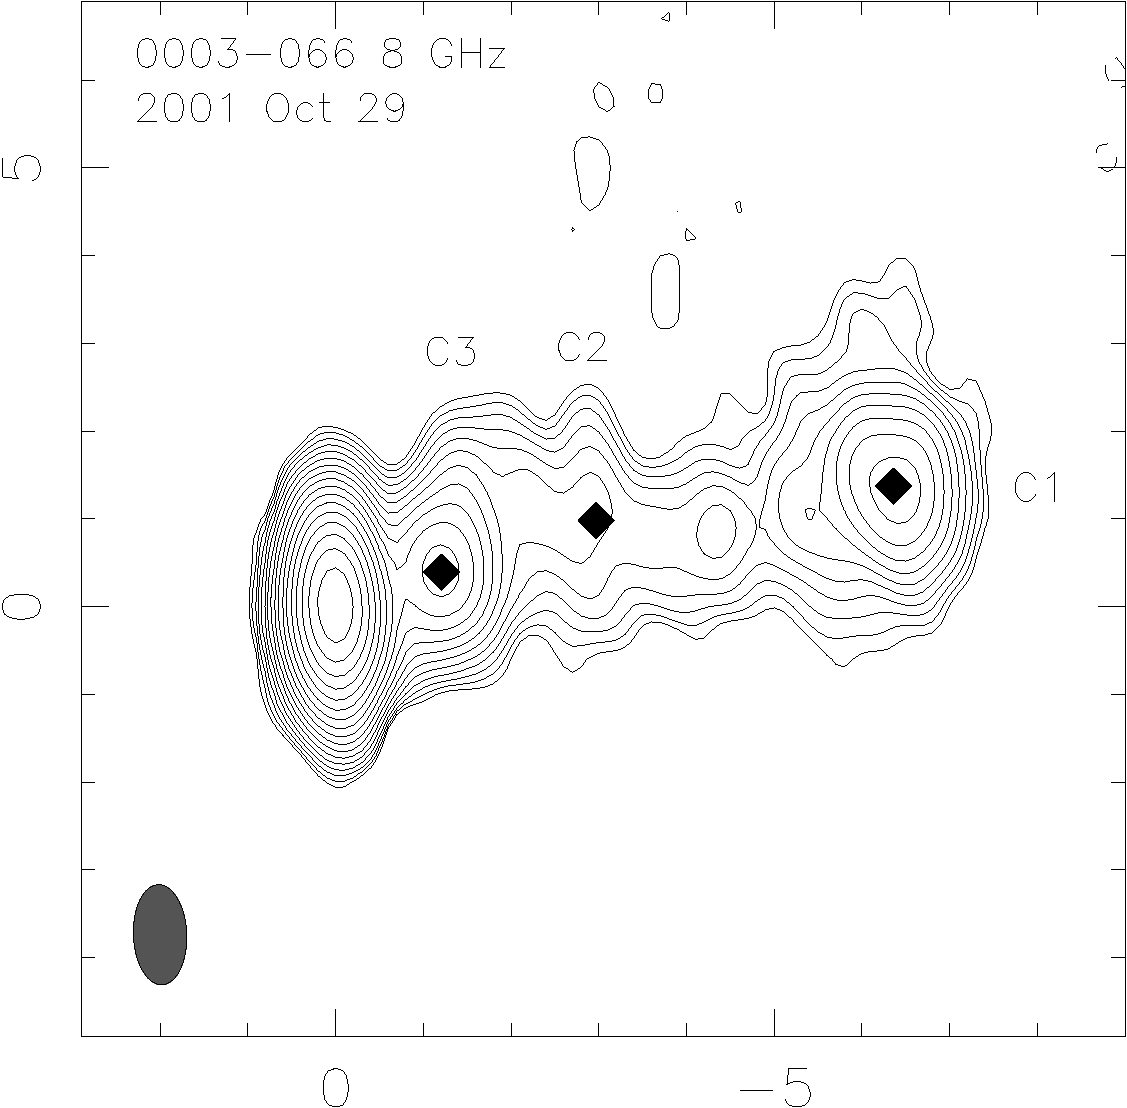
\includegraphics[width=0.7\textwidth]{rdv_0003-066.pdf}
 }
 \caption{Изображение 0003\textminus066 от 29 октября 2001 года из RDV30. По осям отложены
миллисекунды дуги. Самый низкий контур имеет уровень в три раза превышающий уровень шума
\SI{0.9}{\milli\jansky\per\beam}, и каждый последующий контур в корень из двух раз больше. Пиковая
плотность потока составляет \SI{0.96}{\jansky\per\beam}. Размер диаграммы направленности
равен 1.14 на \SI{0.61}{\mas} при позиционном угле \ang{2.3} и показан в
левом нижнем углу изображения. Три залитых ромба указывают на детали струи, которые следовали
модели Гаусса. Параметры гауссовых моделей приведены в таблице~\ref{tab:rdv_mfit}.}
 \label{fig:0003}
\end{figure}

После самокалибровки и построения изображений к видностям, ассоциированным с каждым изображением,
подгонялись Гауссовы модели с помощью задачи \emph{modelfit} в DIFMAP. Такие модели Гауссовы
обеспечивают лаконичное математическое описание положения и свойств различных компонентов
струи на каждом изображении. Подгонка модели в плоскости видимости по сравнению с плоскостью
изображения позволяет достичь разрешения лучше диаграммы направленности в случаях высокого
отношения сигнал/шум; см. также обсуждение подгонки модели в плоскости видностей по сравнению с
подгонкой в плоскости изображения в \cite{Lister_2009b} и предела разрешения в плоскости видности
в \cite{Kovalev_2005}.

Наша процедура подгонки модели была подробно описана в \cite{Piner_2007}, но мы рассмотрим и
суммируем ее здесь. Точное количество используемых гауссовых компонентов и выбор между
эллиптическими или круговыми гауссианами могут быть субъективными, но в данном случае мы исходили из
простоты полученной модели и согласованности модели для данного источника от эпохи к эпохе.
Эллиптические компоненты использовались редко, и только для ядра или яркого компонента струи, когда
остатки, оставшиеся от круговой гауссовой подгонки, были настолько велики, что препятствовали
дальнейшей подгонке модели с использованием карты невязок. Чтобы сохранить последовательность от
эпохи к эпохе, финальная модель из предыдущей или более поздней эпохи часто использовалась в
качестве нулевого приближения для рассматриваемой эпохи. Изредка некоторые подгонки модели из
\cite{Piner_2007} переделывались для согласованности с более поздними эпохами. Подгруппа источников
была смоделирована независимо несколькими авторами для проверки согласованности результатов, и были
получены согласованные результаты кинематики разными моделерами в подавляющем большинстве
($\sim$95\%) случаев. Однако, несмотря на все меры предосторожности, подгонки РСДБ модели не
являются уникальными и представляют только одну математически возможную деконволюцию сложной
структуры источника (см., например, сравнение результатов RDV и 2-см обзора из статьи
\cite{Piner_2007}).

\begin{table}[]
\caption{Гауссовы модели}
\label{tab:rdv_mfit}
\centering
\tiny
\begin{SingleSpace}
\begin{tabular}{l S S S S S S S S S S S S}
\toprule
Источник & {$S$} & {$r$} & {P.A.} & {$a$} & {$(b/a)$} & {P.A.$_\text{maj}$} & Тип & Эпоха &
Компонент & {$a_\text{beam}$} & {$b_\text{beam}$} & {$\theta_\text{beam}$} \\
 & {(\si{\jansky})} & {(\si{\mas})} & {(\si{\degree})}
& {(\si{\mas})} &  & {(\si{\degree})} &  &  &  & {(\si{\mas})} & {(\si{\mas})} & {(\si{\mas})} \\
\multicolumn{1}{c}{(1)} & {(2)} & {(3)} & {(4)} & {(5)} & {(6)} & {(7)} & {(8)} & {(9)} & {(10)} &
{(11)} & {(12)} & {(13)} \\
\midrule
0003\textminus066 & 1.599 & 0.079 &   148.3 & 0.633 & 0.387 & -16.3 & 1 & 1995.78 &  0 &
2.29 & 0.95 & -1.1 \\
           & 0.645 & 1.040 & -60.5 & 1.384 & 1.000 &     0.0 & 1 &         & 99 &      &
  &    \\
           & 0.156 & 5.145 & -74.5 & 3.222 & 1.000 &     0.0 & 1 &         &  1 &      &
  &    \\
           & 1.209 & 0.032 & 114.2 & 0.529 & 0.000 &    21.2 & 1 & 1997.08 &  0 & 2.03 & 0.75 &
-5.8 \\
           & 0.225 & 0.786 & -48.9 & 0.520 & 1.000 &     0.0 & 1 &         &  3 &      &
  &    \\
           & 0.194 & 2.131 & -71.1 & 1.416 & 1.000 &     0.0 & 1 &         &  2 &      &
  &    \\
           & 0.083 & 5.586 & -75.2 & 2.455 & 1.000 &     0.0 & 1 &         &  1 &      &
  &    \\
\bottomrule
\end{tabular}
\end{SingleSpace}

\textbf{Примечания.}
Колонка 1: имя источника B1950.
Колонка 2: плотность потока в Янских.
Колонки 3 and 4: $r$ and P.A. (позиционный угол)~"---полярные координаты центра Гауссианы.
Позиционный угол отсчитывается от севера на восток.
Колонки 5--7: $a$ и $b$~"--- это ширина на половине максимума (FWHM) большой и малой оси Гауссианы,
а P.A.$_\text{maj}$~"--- позиционный угол большой оси. Для круглых компонентов $(b/a)$ и
P.A.$_\text{maj}$ равны 1.0 и 0.0 соответственно.
Колонка 8: тип компонента для команды <<modelfit>> из DIFMAP. Тип 1 обозначает гауссовый компонент.
Тип 0~"--- дельта-функцию.
Колонка 9: эпоха наблюдения.
Компонент 10: номер компонента. Компонент <<0>> обозначает предполагаемое ядро. Остальные
компоненты пронумерованы от 1 до 11, от внешних к внутренним. Номер <<99>> обозначает компонент,
которые не используется в анализе.
Колонки 11--13: $a_\text{beam}$, $b_\text{beam}$ и $\theta_\text{beam}$ --- это FWHM большой оси,
FWHM малой оси и позиционный угол большой оси диаграммы направленности при натуральном взвешивании
(uvweight 0,\textminus1~в DIFMAP).
\end{table}

Полные результаты подбора гауссовой модели представлены в машиночитаемой форме в
таблице~\ref{tab:rdv_mfit}. Таблица~\ref{tab:rdv_mfit} содержит в общей сложности 8571 гауссовых
компонентов, подогнанных к 2753 изображениям, или в среднем около 3 компонентов на изображение (ядро
и два компонента струи). Столбцы 2--8 таблицы~\ref{tab:rdv_mfit} непосредственно соответствуют
результатам работы \emph{modelfit} из DIFMAP и подходят для непосредственного считывания в DIFMAP с
помощью команды \emph{rmodel}. Положение компонентов в таблице~\ref{tab:rdv_mfit} не были смещены,
чтобы поместить ядро в начало координат, так что положения в таблице~\ref{tab:rdv_mfit}
непосредственно соответствуют позициям на общедоступных изображениях. Обратите внимание, что
измерения плотности потока в столбце 2 не очень точны в случае относительно близко расположенных
компонентов, где разделение плотности потока между компонентами может быть неоднозначным.

После после моделирования всех эпох данного источника, компоненты струи должны были быть перекрестно
идентифицированы от эпохи к эпохе, чтобы изучить их кинематику. Эта идентификация компонента
приведена в столбце 10 таблицы~\ref{tab:rdv_mfit}. Компонент <<0>> указывает на предполагаемое ядро.
Другие компоненты пронумерованы от 1 до 11, от самого внешнего компонента внутрь. Идентификатор
компонента <<99>> указывает на неопознанный компонент, не использованный в анализе. Мы
идентифицируем ядро в каждом источнике как компактный компонент в конце структуры односторонней
струи "--- часто, но не всегда, это также самый яркий компонент. Как отмечалось выше, мы исключили
источники, которые, как известно, показывают двусторонние РСДБ структуры на этих масштабах.
Идентификация компонентов струи была сделана на основе согласованности потока, расстояния,
позиционного угла и размера от эпохи к эпохе. Ожидается, что при таком большом количестве эпох на
источник, которые используются здесь, и близком интервале времени, такая идентификация будет
надежной. В тех случаях, когда компонент модели не мог быть непосредственно идентифицирован с
компонентами модели, замеченными в другие эпохи, ему присваивался номер <<99>> в
таблице~\ref{tab:rdv_mfit}, чтобы пометить его как компонент модели, не используемый в анализе. Это
обычно происходило, когда на изображении с несколько более низким разрешением смешивалось вместе то,
что рассматривалось как два отдельных компонента в других моделях (<<слияние>>), или когда компонент
с низким динамическим диапазоном был обнаружен только в нескольких изображениях с плохо ограниченным
положением.

Некоторые общие статистические данные по подгонкам в таблице~\ref{tab:rdv_mfit} приведены ниже. Из
общего числа 8571 компонента 2753 являются ядрами, а 5818~"--- компонентами струи. Около 84\,\%
компонентов (7205) являются круговыми гауссианами, в то время как около 16\% (1366)~"---
эллиптическими. Из 1366 эллиптических гауссианов 1277 (около 93\%) были использованы для
моделирования ядра, в то время как только 89 (около 7\%) использовались для моделирования
компонентов струи. Это означает, что около 46\% компонентов ядра представлены эллипсами, в то время
как только около 2\% компонентов струи представлены эллипсами. Когда ядро моделируется
эллиптическим компонентом, то угол положения большой оси имеет тенденцию выравниваться с углом
положения струи, как показано на рисунке~\ref{fig:rdv_pos_ang_diff}. На этом рисунке показана
гистограмма разницы между углом положения большой оси эллиптического ядра и позиционным углом
ближайшего компонента струи, для 1125 эллиптических ядер с последующим компонентом струи,
смоделированным в ту же эпоху. Избыток при небольших смещениях очевиден, что позволяет предположить,
что эллиптические компоненты ядра моделируют начало структуры удлиненной струи. Аналогичный
результат был найден для компонентов эллиптического ядра для обзора 2 см \cite{Kovalev_2005}.

\begin{figure}[]
 \centerfloat{
  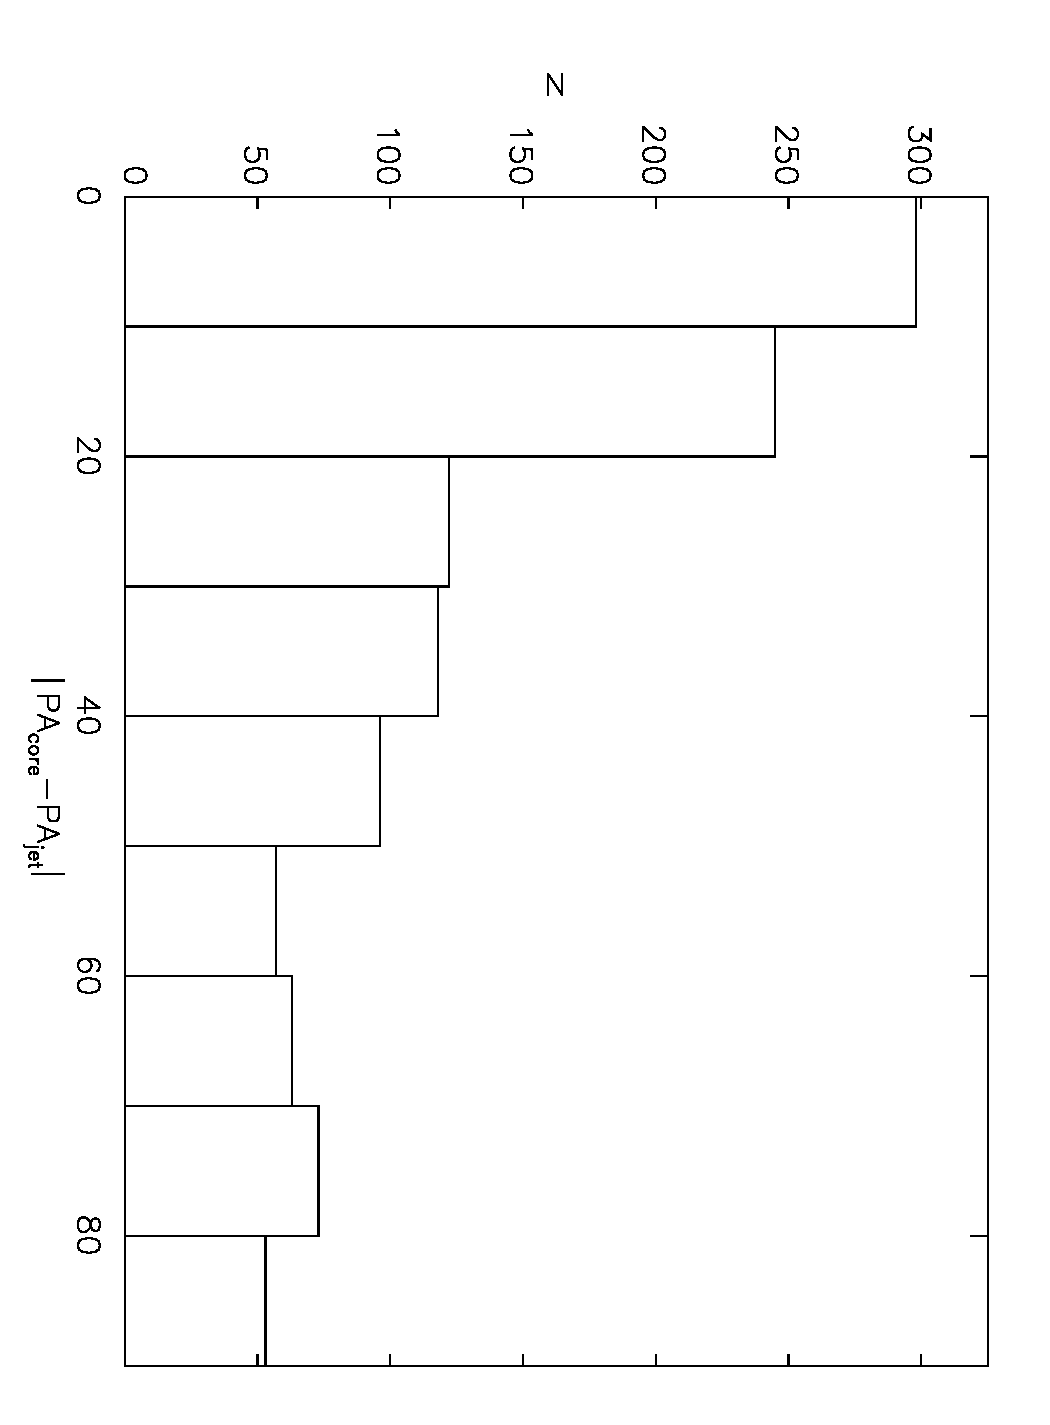
\includegraphics[height=0.7\textwidth,angle=90]{rdv_pos_ang_diff.pdf}
 }
 \caption{Гистограмма разности между позиционным углом большой оси эллиптического ядра
и позиционными углом ближайшего компонента струи, расположенного ниже по потоку.}
 \label{fig:rdv_pos_ang_diff}
\end{figure}

Из 5818 компонентов струи в таблице~\ref{tab:rdv_mfit} 5069 (около 87\,\%) были идентифицированы с
определенным идентификатором компонента в столбце 10 таблицы~\ref{tab:rdv_mfit}, в то время как 749
(около 13\,\%) не идентифицированы (идентификатор <<99>> в столбце 10). Всего имеется 225 уникальных
компонентов струи, по крайней мере, с четырьмя эпохами наблюдения (которые нам необходимы для
кинематического анализа), идентифицированных в 66 источниках в таблице~\ref{tab:rdv_mfit}. При 5069
общих наблюдениях идентифицированных компонентов струи это дает в среднем около 23 наблюдений
каждого из 225 уникальных компонентов.

\begin{table}
\caption{Сравнение обзоров MOJAVE и RDV}
\label{tab:rdv_comptab}
\small
\centering
\begin{tabular}{l c c}
\toprule
Показатель & MOJAVE$^{a}$ & RDV \\
\midrule
Общее количество источников                             & 135  & 68   \\
Количество источников в собственным движением           & 127  & 66   \\
Общее количество изображений                            & 2424 & 2753 \\
%Median number of images per source              & 15   & 43   \\
%Minimum number of images per source             & 5    & 20   \\
Общая продолжительность обзора (годы)                   & 13   & 10   \\
Средний промежуток между изображениями источника (годы) & 0.7  & 0.2  \\
Количество компонентов                                  & 526  & 225  \\
\bottomrule
\end{tabular}

\textbf{Примечания.}
$a$: Использованы опубликованные изображения и кинематика из обзора
MOJAVE~\cite{Lister_2009a,Lister_2009b}.
\end{table}

В таблице~\ref{tab:rdv_comptab} показано сравнение некоторых важных свойств обзора RDV по сравнению
с обзором MOJAVE, опубликованным \cite{Lister_2009a,Lister_2009b}. В то время как общее количество
изображений одинаково для двух обзоров, в обзоре MOJAVE было изучено примерно вдвое больше
источников, и общее количество компонентов примерно в два раза больше, чем в обзоре RDV. Тем не
менее, обзор RDV имеет более высокое среднее число изображений на источник и меньший средний
временной промежуток между изображениями, что полезно для изучения кинематики струи, включая анализ
ускорения.


\subsection{Видимые скорости}

\subsubsection{Методы подгонки}

Мы провели два типа подгонки к каждому из 225 данных о положении компонентов во времени, чтобы
изучить кинематику струи. Первая подгонка была линейной подгонкой $r$ от $t$ с двумя свободными
параметрами. Эти подгонки дают собственное движение как скорость изменения $r$, равную наклону
линии наилучшего соответствия на графике расстояния от времени, и они позволяют проводить прямое
сравнение с измерениями видимой скорости из статьи \cite{Piner_2007}.

Второй тип подгонки был полином второго порядка для $x(t)$ и $y(t)$ отдельно для каждого компонента
и предоставляет информацию о кажущемся ускорении каждого компонента. Используемый здесь метод
нелинейной аппроксимации идентичен методу, описанному \cite{Homan_2001}, а затем использовался в
измерениях ускорения в обзоре MOJAVE \cite{Lister_2009b,Homan_2009}. Мы используем ту же
параметризацию для подгонки, что и \cite{Homan_2001} и \cite{Homan_2009}, что позволяет проводить
прямое сравнение наших результатов с результатами ускорения в MOJAVE. Мы суммируем этот нелинейный
метод подгонки ниже.

В этих нелинейных подгонках используются три параметра для $x(t)$ и $y(t)$, т.\:е. в общей
сложности шесть свободных параметров для каждого компонента. Вектор собственного движения
для каждой подгонки определяется из среднего собственного движения в направлениях $x$ и $y$
($\mu_x$ и $\mu_y$) или, что эквивалентно, вектора собственного движения в середине времени
$t_\text{mid} = (t_i + t_f) / 2$, где $t_i$ и $t_f$~"--- времена начального и конечного наблюдения
компонента, соответственно. Величина среднего вектора собственного движения
обозначается $\mu$, а направление этого вектора~"--- $\phi$. Величина $\mu$ затем преобразуется в
наблюдаемую кажущуюся скорость $\beta_\text{app}$. Величина $|\text{P.A.} - \phi|$ дает разность
между средневзвешенным позиционным углом P.A. компонента и направлением вектора его средней видимой
скорости.

Кажущееся угловое ускорение вычисляется из $\ddot{x}$ и $\ddot{y}$ ($\dot{\mu}_x$ и $\dot{\mu}_y$).
Это кажущееся угловое ускорение раскладывается на две составляющие, параллельные и перпендикулярные
направлению номинальной скорости $\phi$. Эти два компонента обозначены $\dot{\mu}_{\parallel}$ и
$\dot{\mu}_{\perp}$, и они представляют кажущееся угловое ускорение из-за изменений в кажущейся
скорости и из-за изменений направления, соответственно. Чтобы легче было сравнивать кажущиеся
ускорения среди высокоскоростных и низкоскоростных джетов, относительное параллельное ускорение
определяется как
\begin{equation}
\label{eq:rdv_relpar}
\dot{\eta}_{\parallel}\equiv
\dot{\beta}_\mathrm{\parallel app}/\beta_\mathrm{app}=(1+z)\dot{\mu}_{\parallel}/\mu\,,
\end{equation}
а относительное перпендикулярное ускорение определяется как
\begin{equation}
\label{eq:rdv_relperp}
\dot{\eta}_{\perp}\equiv
\dot{\beta}_\mathrm{\perp app}/\beta_\mathrm{app}=(1+z)\dot{\mu}_{\perp}/\mu\,.
\end{equation}
Таким образом, компонент с относительным параллельным ускорением 0.1, например, имеет кажущуюся
скорость, которая увеличивается на 10\,\% в год. Отметим также, что относительное ускорение,
определенное таким образом, имеет размерность обратного времени. Эти подгонки предполагают
постоянное ускорение в течение времени наблюдения за компонентом, хотя мы не можем исключать
возможность того, что более сложные и переменные во времени ускорения также могут иметь место.

Для обоих методов подгонки (линейного и нелинейного) ошибки в измерениях положения были определены
в соответствии с методом, описанным в \cite{Homan_2001} и впоследствии используется в
\cite{Lister_2009b,Homan_2009}. Этот метод использует разброс точек вокруг подгонки, чтобы
назначить постоянную погрешность для каждой точки, такой что значение $\chi^{2}$
подгонки имело значение 1.0. Это отличается от метода на основе диаграммы направленности для
назначения позиционных ошибок, который мы использовали в статье \cite{Piner_2007}. Новый метод
имеет тот недостаток, что значение $\chi^{2}$ нельзя использовать для определения пригодности
выбранной модели, но при условии, что модель уместно, это дает хорошие неопределенности для
параметров модели. В нем также прямо рассматривается хорошо известная проблема в РСДБ моделировании,
которая заключается в том, что при большом количестве измерений положения не существует метода для
получения надежных и статистически точных неопределенностей, которые будут работать для всех
компонентов в наборе данных, и будут приняты во внимание как ошибки, вызванные погрешностями
измерений видности, так и систематические эффекты, вызванные изменениями в количестве и форме
компонентов модели, или эффектами, введенными во время калибровки и построения изображений.

\begin{figure}[]
 \centerfloat{
  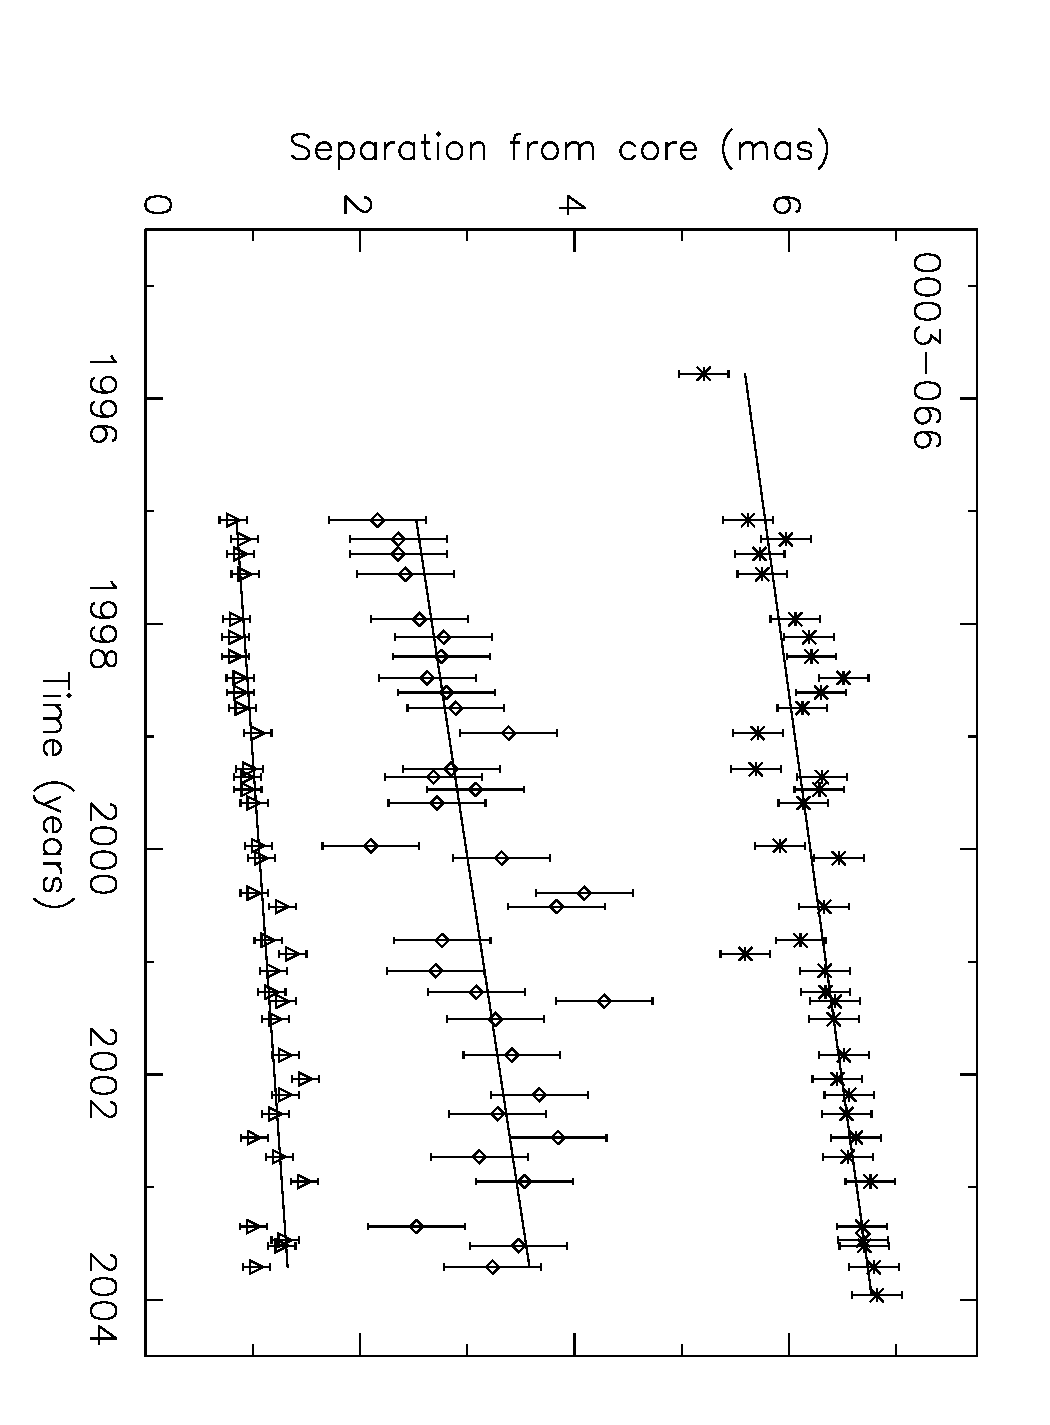
\includegraphics[height=0.7\textwidth,angle=90]{rdv_f3.pdf}
 }
 \caption{Угловое расстояние от ядра центров гауссовых компонент как функция времени.
Прямые линии~"--- линейная подгонка методом наименьших квадратов радиального движения с постоянной
скоростью для компонентов, обнаруженных в четырех или более эпохах. Для каждого источника
звездочками обозначен компонент 1, ромбами компонент 2, треугольниками компонент 3, квадратами
компонент 4, $\times$-ми компонент 5 и кружками компонент 6. Затем этот цикл символов
повторяется, начиная с компонента 7. Неопознанные компоненты из таблицы~\ref{tab:rdv_mfit} не
показаны. Некоторые столбики ошибок меньше, чем графические символы. Название источника B1950
указано в левом верхнем углу каждой панели.}
 \label{fig:rdv_sep}
\end{figure}

\begin{table*}
\caption{Видимая скорость компонентов из линейной подгонки}
\label{tab:rdv:speedtab}
\scriptsize
\centering
\begin{SingleSpace}
\begin{tabular}{l c r r r r c}
\toprule
\multicolumn{1}{c}{Источник} & Комп. & \multicolumn{1}{c}{$\langle{S}\rangle$} &
\multicolumn{1}{c}{$\langle{r}\rangle$} & \multicolumn{1}{c}{$\mu$}
& \multicolumn{1}{c}{$\beta_\mathrm{app}$} & \multicolumn{1}{c}{$t_{0}^{a}$} \\
 & & \multicolumn{1}{c}{(Ян)} & \multicolumn{1}{c}{(\si{\mas})}
& \multicolumn{1}{c}{(\si{\uas\per\year})} &  &
\multicolumn{1}{c}{(год)} \\
\multicolumn{1}{c}{(1)} & \multicolumn{1}{c}{(2)} & \multicolumn{1}{c}{(3)} &
\multicolumn{1}{c}{(4)} & \multicolumn{1}{c}{(5)} &
\multicolumn{1}{c}{(6)} & \multicolumn{1}{c}{(7)} \\
\midrule

0014+813 &  1 &  0.006 & $ 9.39\pm 0.07$ & $  45\pm  34$ & $  4.9\pm 3.6$ & \dots \\
         &  2 &  0.010 & $ 5.36\pm 0.06$ & $  28\pm  30$ & $  3.0\pm 3.2$ & \dots \\
         &  3 &  0.113 & $ 0.67\pm 0.01$ & $  -5\pm   4$ & $ -0.6\pm 0.4$ & \dots \\
0048$-$097 &  1 &  0.008 & $ 3.09\pm 0.36$ & $ -79\pm 183$ & $ -2.9\pm 6.7$ & \dots \\
         &  3 &  0.022 & $ 0.60\pm 0.04$ & $  32\pm  53$ & $  1.2\pm 1.9$ & \dots \\
         &  4 &  0.063 & $ 0.86\pm 0.09$ & $ 339\pm 191$ & $ 12.4\pm 7.0$ & \dots \\
         &  5 &  0.137 & $ 0.67\pm 0.06$ & $ 178\pm  70$ & $  6.5\pm 2.6$ & \dots \\
0119+115 &  1 &  0.023 & $20.33\pm 0.11$ & $ 284\pm 143$ & $  9.5\pm 4.8$ & \dots \\
         &  2 &  0.009 & $14.24\pm 0.08$ & $  61\pm  93$ & $  2.0\pm 3.1$ & \dots \\
         &  3 &  0.105 & $ 1.64\pm 0.05$ & $ 242\pm  23$ & $  8.1\pm 0.8$ & $1993.53\pm   0.65$ \\
         &  4 &  0.247 & $ 1.39\pm 0.04$ & $ 317\pm  43$ & $ 10.6\pm 1.4$ & $1998.15\pm   0.61$ \\
0458$-$020 &  1 &  0.070 & $ 4.57\pm 0.07$ & $ 296\pm  35$ & $ 26.6\pm 3.1$ & $1984.97\pm   1.85$ \\
         &  2 &  0.121 & $ 1.78\pm 0.05$ & $ 198\pm  23$ & $ 17.8\pm 2.1$ & $1991.21\pm   1.06$ \\
0528+134 &  1 &  0.090 & $ 3.66\pm 0.04$ & $  75\pm  19$ & $  6.4\pm 1.6$ & $1951.52\pm  13.05$ \\
         &  2 &  0.266 & $ 1.43\pm 0.02$ & $ 125\pm  11$ & $ 10.7\pm 0.9$ & $1989.09\pm   0.99$ \\
         &  3 &  0.564 & $ 0.46\pm 0.01$ & $   5\pm   7$ & $  0.4\pm 0.6$ & \dots \\
         &  4 &  1.166 & $ 0.23\pm 0.04$ & $ 201\pm 133$ & $ 17.1\pm11.3$ & \dots \\
0642+449 &  1 &  0.012 & $ 3.41\pm 0.06$ & $  -5\pm  27$ & $ -0.5\pm 2.9$ & \dots \\
         &  3 &  0.708 & $ 0.28\pm 0.01$ & $  -8\pm   3$ & $ -0.9\pm 0.3$ & \dots \\
0823+033 &  1 &  0.015 & $ 9.80\pm 0.21$ & $ 655\pm 235$ & $ 19.9\pm 7.1$ & \dots \\
         &  2 &  0.038 & $ 4.05\pm 0.08$ & $ 122\pm  63$ & $  3.7\pm 1.9$ & \dots \\
         &  3 &  0.090 & $ 2.62\pm 0.03$ & $ -13\pm  14$ & $ -0.4\pm 0.4$ & \dots \\
         &  4 &  0.164 & $ 1.02\pm 0.02$ & $  59\pm  11$ & $  1.8\pm 0.3$ & $1982.21\pm   3.43$ \\
         &  5 &  0.106 & $ 0.59\pm 0.03$ & $ 131\pm  38$ & $  4.0\pm 1.1$ & $1997.89\pm   1.41$ \\
         &  6 &  0.304 & $ 0.33\pm 0.02$ & $ -58\pm  65$ & $ -1.8\pm 2.0$ & \dots \\
0851+202 &  1 &  0.023 & $ 3.61\pm 0.12$ & $  40\pm  84$ & $  0.8\pm 1.6$ & \dots \\
         &  2 &  0.104 & $ 2.55\pm 0.07$ & $ 344\pm  27$ & $  6.7\pm 0.5$ & $1992.84\pm   0.58$ \\
         &  3 &  0.125 & $ 1.21\pm 0.03$ & $ 230\pm  32$ & $  4.5\pm 0.6$ & $1994.10\pm   0.75$ \\
         &  4 &  0.364 & $ 0.92\pm 0.03$ & $ 199\pm  16$ & $  3.9\pm 0.3$ & $1996.66\pm   0.38$ \\
         &  5 &  0.420 & $ 0.67\pm 0.03$ & $ 258\pm  25$ & $  5.0\pm 0.5$ & $1999.85\pm   0.25$ \\
0919$-$260 &  1 &  0.020 & $ 6.14\pm 0.09$ & $ 146\pm  43$ & $ 13.2\pm 3.9$ & $1957.71\pm  13.52$ \\
         &  2 &  0.038 & $ 2.02\pm 0.21$ & $-137\pm 172$ & $-12.4\pm15.5$ & \dots \\
         &  3 &  0.118 & $ 1.39\pm 0.04$ & $ 121\pm  16$ & $ 10.9\pm 1.4$ & $1988.74\pm   1.57$ \\
0923+392 &  1 &  1.103 & $ 2.52\pm 0.05$ & $   6\pm  44$ & $  0.2\pm 1.7$ & \dots \\
         &  2 &  7.089 & $ 2.11\pm 0.02$ & $  52\pm   9$ & $  2.1\pm 0.3$ & $1959.29\pm   7.07$ \\
         &  3 &  1.851 & $ 1.46\pm 0.03$ & $ 164\pm  15$ & $  6.5\pm 0.6$ & $1991.62\pm   0.81$ \\
1101+384 &  1 &  0.016 & $ 5.38\pm 0.09$ & $ -79\pm  41$ & $ -0.2\pm 0.1$ & \dots \\
         &  2 &  0.012 & $ 2.84\pm 0.06$ & $ -58\pm  27$ & $ -0.1\pm 0.1$ & \dots \\
         &  3 &  0.027 & $ 1.46\pm 0.03$ & $  23\pm  15$ & $  0.05\pm 0.03$ & \dots \\
         &  4 &  0.061 & $ 0.55\pm 0.02$ & $   2\pm   9$ & $  0.004\pm 0.019$ & \dots \\
1124$-$186 &  1 &  0.011 & $ 2.70\pm 0.20$ & $ 500\pm 122$ & $ 27.3\pm 6.7$ & $1993.11\pm   1.40$ \\
         &  2 &  0.072 & $ 0.87\pm 0.05$ & $  41\pm  23$ & $  2.3\pm 1.3$ & \dots \\
1145$-$071 &  1 &  0.103 & $ 2.20\pm 0.01$ & $  52\pm   6$ & $  3.4\pm 0.4$ & $1958.15\pm   4.55$ \\
1156+295 &  1 &  0.049 & $ 7.22\pm 0.27$ & $ -75\pm 207$ & $ -3.1\pm 8.5$ & \dots \\
         &  2 &  0.080 & $ 6.29\pm 0.08$ & $ 636\pm  37$ & $ 26.2\pm 1.5$ & $1990.38\pm   0.58$ \\
         &  3 &  0.117 & $ 2.24\pm 0.11$ & $ 494\pm  49$ & $ 20.3\pm 2.0$ & $1995.61\pm   0.46$ \\
         &  5 &  0.209 & $ 0.56\pm 0.03$ & $  50\pm  19$ & $  2.1\pm 0.8$ & \dots \\
1228+126 &  1 &  0.125 & $21.37\pm 0.29$ & $-114\pm 142$ & $ -0.03\pm 0.04$ &  ... \\
         &  2 &  0.096 & $11.54\pm 0.24$ & $  63\pm 120$ & $  0.02\pm 0.03$ & ... \\
         &  3 &  0.108 & $ 6.57\pm 0.07$ & $  88\pm  36$ & $  0.02\pm 0.01$ & ... \\
         &  4 &  0.140 & $ 2.97\pm 0.08$ & $  90\pm  39$ & $  0.02\pm 0.01$ & ... \\
         &  5 &  0.285 & $ 1.48\pm 0.04$ & $  -4\pm  22$ & $ -0.001\pm 0.006$ &  ... \\
         &  6 &  0.336 & $ 0.57\pm 0.02$ & $   6\pm  11$ & $  0.001\pm 0.003$ &  ... \\
1313$-$333 &  1 &  0.028 & $ 7.45\pm 0.07$ & $ 704\pm 115$ & $ 42.6\pm 7.0$ & $1989.58\pm   1.78$ \\
         &  2 &  0.049 & $ 2.02\pm 0.05$ & $ 383\pm  68$ & $ 23.2\pm 4.1$ & $1992.65\pm   0.97$ \\
         &  3 &  0.121 & $ 2.08\pm 0.07$ & $ 497\pm  34$ & $ 30.1\pm 2.1$ & $1996.27\pm   0.29$ \\
1611+343 &  1 &  0.573 & $ 3.59\pm 0.03$ & $  60\pm  15$ & $  4.0\pm 1.0$ & $1940.33\pm  16.37$ \\
         &  2 &  0.204 & $ 4.03\pm 0.02$ & $ 108\pm  18$ & $  7.2\pm 1.2$ & $1963.53\pm   6.33$ \\
         &  3 &  0.350 & $ 2.84\pm 0.01$ & $  25\pm   4$ & $  1.7\pm 0.3$ & $1886.21\pm  19.59$ \\
         &  4 &  0.099 & $ 1.38\pm 0.03$ & $ 183\pm  18$ & $ 12.3\pm 1.2$ & $1992.17\pm   0.73$ \\
         &  5 &  0.386 & $ 0.73\pm 0.01$ & $ 214\pm   8$ & $ 14.3\pm 0.6$ & $1997.78\pm   0.13$ \\
         &  6 &  0.730 & $ 0.49\pm 0.03$ & $ 333\pm  55$ & $ 22.3\pm 3.7$ & $2001.49\pm   0.25$ \\
1745+624 &  1 &  0.007 & $ 2.58\pm 0.07$ & $  76\pm  30$ & $  8.7\pm 3.5$ & ... \\
         &  2 &  0.015 & $ 1.46\pm 0.03$ & $  64\pm  17$ & $  7.4\pm 1.9$ & $1976.72\pm   6.44$ \\
         &  3 &  0.018 & $ 1.10\pm 0.05$ & $ 132\pm  62$ & $ 15.1\pm 7.1$ & ... \\
         &  4 &  0.035 & $ 0.55\pm 0.05$ & $  70\pm  54$ & $  8.1\pm 6.3$ & ... \\
         &  5 &  0.287 & $ 0.24\pm 0.01$ & $  10\pm   3$ & $  1.2\pm 0.4$ & $1977.39\pm   7.75$ \\
1803+784 &  1 &  0.040 & $ 7.15\pm 0.09$ & $ -56\pm  42$ & $ -2.2\pm 1.6$ & ... \\
         &  2 &  0.051 & $ 3.45\pm 0.08$ & $  80\pm  38$ & $  3.1\pm 1.5$ & ... \\
         &  3 &  0.083 & $ 1.83\pm 0.02$ & $ -38\pm   9$ & $ -1.5\pm 0.4$ & ... \\
         &  4 &  0.217 & $ 1.44\pm 0.01$ & $ -22\pm   5$ & $ -0.8\pm 0.2$ & ... \\
         &  5 &  0.118 & $ 1.03\pm 0.02$ & $   1\pm  14$ & $  0.04\pm 0.54$ & ... \\
         &  6 &  0.257 & $ 0.47\pm 0.01$ & $  22\pm   7$ & $  0.9\pm 0.3$ & $1979.21\pm   7.09$ \\
2200+420 &  1 &  0.098 & $ 7.71\pm 0.17$ & $ 993\pm 130$ & $  4.6\pm 0.6$ & $1990.81\pm   1.03$ \\
         &  2 &  0.118 & $ 7.47\pm 0.11$ & $ 572\pm  98$ & $  2.6\pm 0.5$ & $1988.62\pm   2.31$ \\
         &  3 &  0.281 & $ 3.93\pm 0.08$ & $ 666\pm 123$ & $  3.1\pm 0.6$ & $1992.39\pm   1.13$ \\
         &  4 &  0.359 & $ 3.06\pm 0.08$ & $ 807\pm  65$ & $  3.7\pm 0.3$ & $1994.60\pm   0.31$ \\
         &  5 &  0.215 & $ 3.98\pm 0.06$ & $ 822\pm  34$ & $  3.8\pm 0.2$ & $1995.60\pm   0.20$ \\
         &  6 &  0.376 & $ 2.82\pm 0.04$ & $ 562\pm  20$ & $  2.6\pm 0.1$ & $1995.19\pm   0.18$ \\
         &  7 &  0.156 & $ 2.11\pm 0.03$ & $ 599\pm  37$ & $  2.8\pm 0.2$ & $1996.66\pm   0.22$ \\
         &  8 &  0.166 & $ 2.23\pm 0.06$ & $ 611\pm  40$ & $  2.8\pm 0.2$ & $1997.86\pm   0.24$ \\
         &  9 &  0.186 & $ 1.97\pm 0.05$ & $ 662\pm  54$ & $  3.1\pm 0.2$ & $1999.45\pm   0.24$ \\
         & 10 &  0.129 & $ 1.28\pm 0.04$ & $ 200\pm  61$ & $  0.9\pm 0.3$ & $1996.39\pm   2.13$ \\
         & 11 &  0.491 & $ 0.34\pm 0.01$ & $ -17\pm   6$ & $ -0.08\pm 0.03$ & ... \\
2243$-$123 &  1 &  0.056 & $10.82\pm 0.08$ & $ -58\pm  41$ & $ -2.1\pm 1.5$ & ... \\
         &  2 &  0.178 & $ 3.33\pm 0.03$ & $  99\pm  13$ & $  3.6\pm 0.5$ & $1966.80\pm   4.40$ \\
         &  3 &  0.480 & $ 1.40\pm 0.01$ & $  87\pm   7$ & $  3.2\pm 0.3$ & $1984.25\pm   1.34$ \\

\bottomrule
\end{tabular}
\end{SingleSpace}
\textbf{Примечания.} (1) имя источника; (2) номер компонента; (3) средняя плотность потока;
(4) средневзвешенное расстояние от ядра; (5) собственное движение; (6) видимая скорость в скоростях
света; (7) время появления компонента дано при значимости собственного движения больше 3$\sigma$.
\end{table*}

Результаты линейных подгонок представлены в таблице~\ref{tab:rdv:speedtab} и показаны в виде
графиков расстояния в зависимости от времени на рисунке~\ref{fig:rdv_sep}.
Таблица~\ref{tab:rdv:speedtab} этой статьи аналогична таблице~4 в \cite{Piner_2007}, но в этой
статье в среднем примерно в четыре раза больше точек на компонент, чем в \cite{Piner_2007}. Таким
образом, мы опустили <<Код качества>>, который мы связали с каждым компонентом в \cite{Piner_2007},
поскольку в данной работе практически все фиты соответствуют качеству <<хорошо>> или <<отлично>>,
как определено в той статье. В таблице~\ref{tab:rdv:speedtab} приведены средняя плотность потока и
средневзвешенное расстояние каждого компонента, собственное радиальное движение и видимая скорость,
а также экстраполированная эпоха, когда компонент отделился от ядра, для компонентов, которые имеют
значимость собственного движения выше $3\sigma$. Полный набор из 66 графиков на
рисунке~\ref{fig:rdv_sep} доступен в онлайн-версии журнала. Линейные подгонки в
таблице~\ref{tab:rdv:speedtab} представлены в основном для соответствия с \cite{Piner_2007}; однако,
большая часть последующего анализа в этой статье использует результаты нелинейных подгонок из
таблицы 6.

\begin{figure}[]
 \centerfloat{
  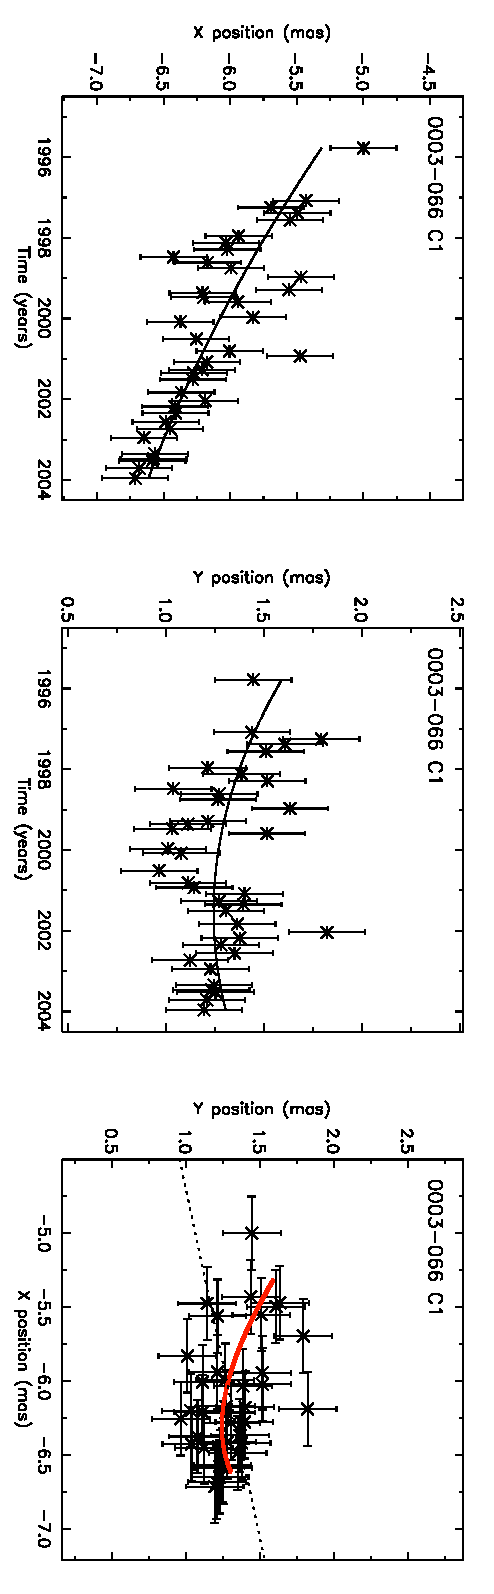
\includegraphics[height=0.95\textwidth,angle=90]{rdv_f4.pdf}
 }
 \caption{На левой и центральной панелях показаны положения $x$ и $y$ соответственно центров
компонентов гауссовой модели относительно ядра как функции времени. Кривые подогнаны методом
наименьших квадратов к $x(t)$ и $y(t)$ для движения с постоянным ускорением для компонентов,
обнаруженных в четыре или более эпохах. На правой панели показаны положения $(x, y)$ центров
компонентов гауссовой модели с левой и центральной панелей. Пунктирная линия показывает радиальное
направление к ядру и от него под средневзвешенным углом положения компонента из таблицы 6.
Подогнанная траектория $(x, y)$ изображена в виде красной кривой для компонентов, которые
являются членами 48- или 64-компонентной подвыборки, которые используются при изучении видимых
ускорений (см. раздел 5). Символы те же, что и на рисунке~\ref{fig:rdv_sep}. Название источника
B1950 и номер компонента указаны в левом верхнем углу каждой панели.}
 \label{fig:rdv_xy}
\end{figure}

Результаты нелинейной подгонки для каждого из 225 компонентов представлены в таблице 6 и графически
показаны на рисунке~\ref{fig:rdv_xy} в виде полиномов второго порядка как $x(t)$, так и $y(t)$ для
каждого компонента в Таблица 6. Полный набор из 225 графиков на рисунке~\ref{fig:rdv_xy} доступен в
онлайн-версии журнала. Обратите внимание, что в колонках 9--14 таблицы 6 не приводятся никакие
записи, если погрешность направления движения >\,\ang{90}. Обычно это происходит
из-за компонентов, которые почти неподвижны, так что направление движения и, следовательно, все
последующие столбцы, которые зависят от направления движения, не определены. Заголовки столбцов в
Таблице 6 идентичны заголовкам в соответствующей таблице в \cite{Homan_2009} (Таблица 1), чтобы
помочь в сравнении между двумя анализами ускорения. Одно из основных отличий между таблицей 6 и
соответствующей таблицей из \cite{Homan_2009} состоит в том, что в таблице 1 из \cite{Homan_2009}
показан анализ ускорения только для высококачественной подвыборки из 203 компонентов, которые
удовлетворяют определенным критериям отбора, из 526 всех компонентов в обзоре MOJAVE. В этой статье
в Таблице 6 представлены подгонки второго порядка для всех 225 компонентов в обзоре RDV, а затем
мы вводим отсечку по качеству данных, аналогичные тем, которые были введены \cite{Homan_2009},
прежде чем проводить анализ ускорения в Разделе 5.

\subsubsection{Изменения скорости в источниках}

\begin{figure}[]
 \centerfloat{
  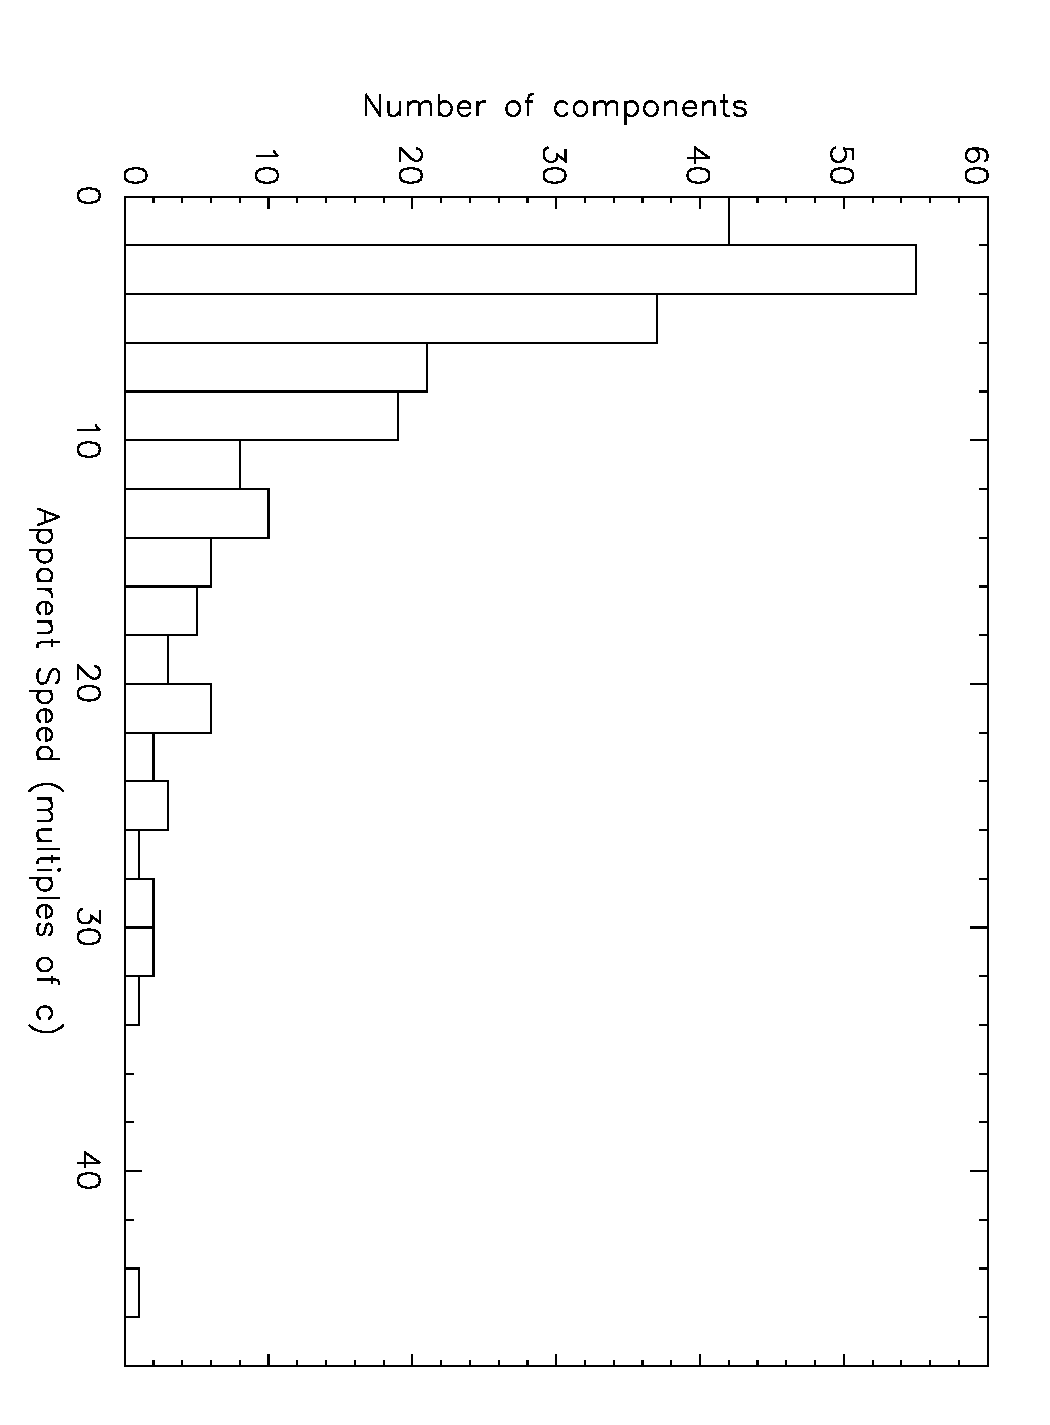
\includegraphics[height=0.7\textwidth,angle=90]{rdv_f5.pdf}
 }
 \caption{Распределение видимой скорости для 224 компонентов в обзоре RDV с измеренными красными
смещениями.}
 \label{fig:rdv_app_speed_distrib}
\end{figure}

На рисунке~\ref{fig:rdv_app_speed_distrib} показана гистограмма измеренной видимой величины скорости
$\beta_\text{app}$ из таблицы 6 для всех компонентов из таблицы 6 ($N = 224$ для 65 источников с
красным смещением; 1657\textminus261 не имеет измеренного красного смещения). Средняя кажущаяся
скорость компонента на рисунке~\ref{fig:rdv_app_speed_distrib} составляет $7.2 c$, а медианная
кажущаяся скорость равна $4.5 c$. Здесь мы обсудим изменение кажущейся скорости от компонента к
компоненту в отдельных источниках, а затем обсудим видимые изменения скорости среди разных
источников в следующем подразделе.

В целом, мы подтверждаем общую тенденцию, наблюдаемую в других исследованиях распределений видимых
скоростей: что, хотя подавляющее большинство компонентов движется наружу, существует также
небольшое, но не пренебрежимо малое количество, по-видимому, движущихся внутрь компонентов и почти
неподвижных компонентов \cite{Lister_2009b,Britzen_2008}. В обзоре RDV 185 из 218 компонентов в
Таблице 6 с измеренным значением $|\text{P.A.} - \phi |$ движутся <<наружу>> ($|\text{P.A.} -
\phi|\leqslant \ang{90}$), в то время как только 33 движутся <<внутрь>> ($|\text{P.A.} - \phi| >
\ang{90}$) "--- и большинство из этих 33 измерений не являются статистически значимыми. Только 10 из
этих 33 компонентов движутся внутрь со значимостью $>3\sigma$, все они также имеют отрицательное
измеренное значение их радиальной кажущейся скорости в таблице~\ref{tab:rdv:speedtab}, как и
ожидалось. В \cite{Lister_2009b} подробно обсуждаются пять различных геометрических эффектов,
которые могут привести к <<иллюзии>> видимого движения внутрь; ни один из них не представляет собой
реальное объемное  движение вещества джета внутрь, и вполне вероятно, что некоторая комбинация этих
пяти эффектов действует на это небольшое подмножество компонентов здесь.

Мы также подтверждаем существование подмножества медленно движущихся или почти неподвижных (Low
Pattern Speed или LPS) компонентов с тем же количеством и расстояниями от ядра, как было
обнаружено в обзоре MOJAVE \cite{Lister_2009b}. В Таблице 6 всего 43 компонента с собственным
движением менее \SI{50}{\uas\per\year}, что является ограничением собственного движения для
компонента LPS в \cite{Lister_2009b}. Из этих 43, 21 также соответствуют двум другим критериям для
компонента LPS, используемого \cite{Lister_2009b}: нет значительного ускорения и скорость
значительно ниже, чем у других компонентов в той же струе. Здесь мы количественно определяем эти два
критерия, так значения $\dot{\eta}_{\parallel}$ и $\dot{\eta}_{\perp}$ должно быть меньше
$2\sigma$, а значение $\beta_\text{app}$ меньше, чем средневзвешенное значение $\beta_\text{app}$
для других компонентов в струе, по крайней мере, на $2\sigma$. 21 компонент в 19 источниках,
которые соответствуют всем трем из этих критериев, отмечены как компоненты LPS в Таблице 6.

С этими критериями компоненты LPS составляют около 9\,\% от компонентов струи в обзоре RDV, и мы
обнаруживаем, что эти компоненты LPS находятся ближе к ядру, чем общая популяция компонентов струи.
Более половины (12 из 21) компонентов LPS сгруппированы на проекционных расстояниях
$\sim\SI{4}{\parsec}$ от ядра (а остальные 9 разбросаны до проецируемых расстояний
$\sim\SI{40}{\parsec}$), в то время как медианная проекция расстояние от ядра для не-LPS
компонентов  составляет \SI{9}{\parsec}. В 8 из 19 источников с компонентами LPS компонент LPS
является ближайшим к ядру. Для сравнения, \cite{Lister_2009b} обнаружили, что общая частота
встречаемости составляет около 6\,\% (31 из 526 компонентов), а типичная проекция расстояния
до ядра составляют менее \SI{9}{\parsec} для компонентов LPS. Такие, по-видимому, стационарные
детали могут быть вызваны проекционными эффектами, если струя проходит очень близко к лучу зрения,
или они могут быть внутренне стационарными деталями, такими как устойчивые реколлимационные
ударные волны, которые ожидаются при моделировании струи (например, \cite{Gomez_1995}), и это может
иметь тенденцию происходить на одинаковых расстояниях от ядра. Тогда в обзоре RDV около 1/6
источников (12 из 66) имеют то, что можно интерпретировать как стационарную деталь, такую как
реколлимационный шок в проекции расстояния $\sim\SI{4}{\parsec}$ от ядра (несколько десятков
парсек de-projected для ожидаемых малых углов обзора). Из 21 LPS компонента 20 находятся в
квазарах, 1~"--- в галактике, и ни один не находится в объектах BL\,Lac, основываясь на оптических
идентификациях в Таблице~\ref{tab:rdv_sources}. В то время как \cite{Lister_2009b} обнаруживает, что
частота появления LPS объектов выше в их объектах BL\,Lac, отметим, что в выборке RDV имеется
только 7 объектов BL\,Lac.

\begin{figure}[]
 \centerfloat{
  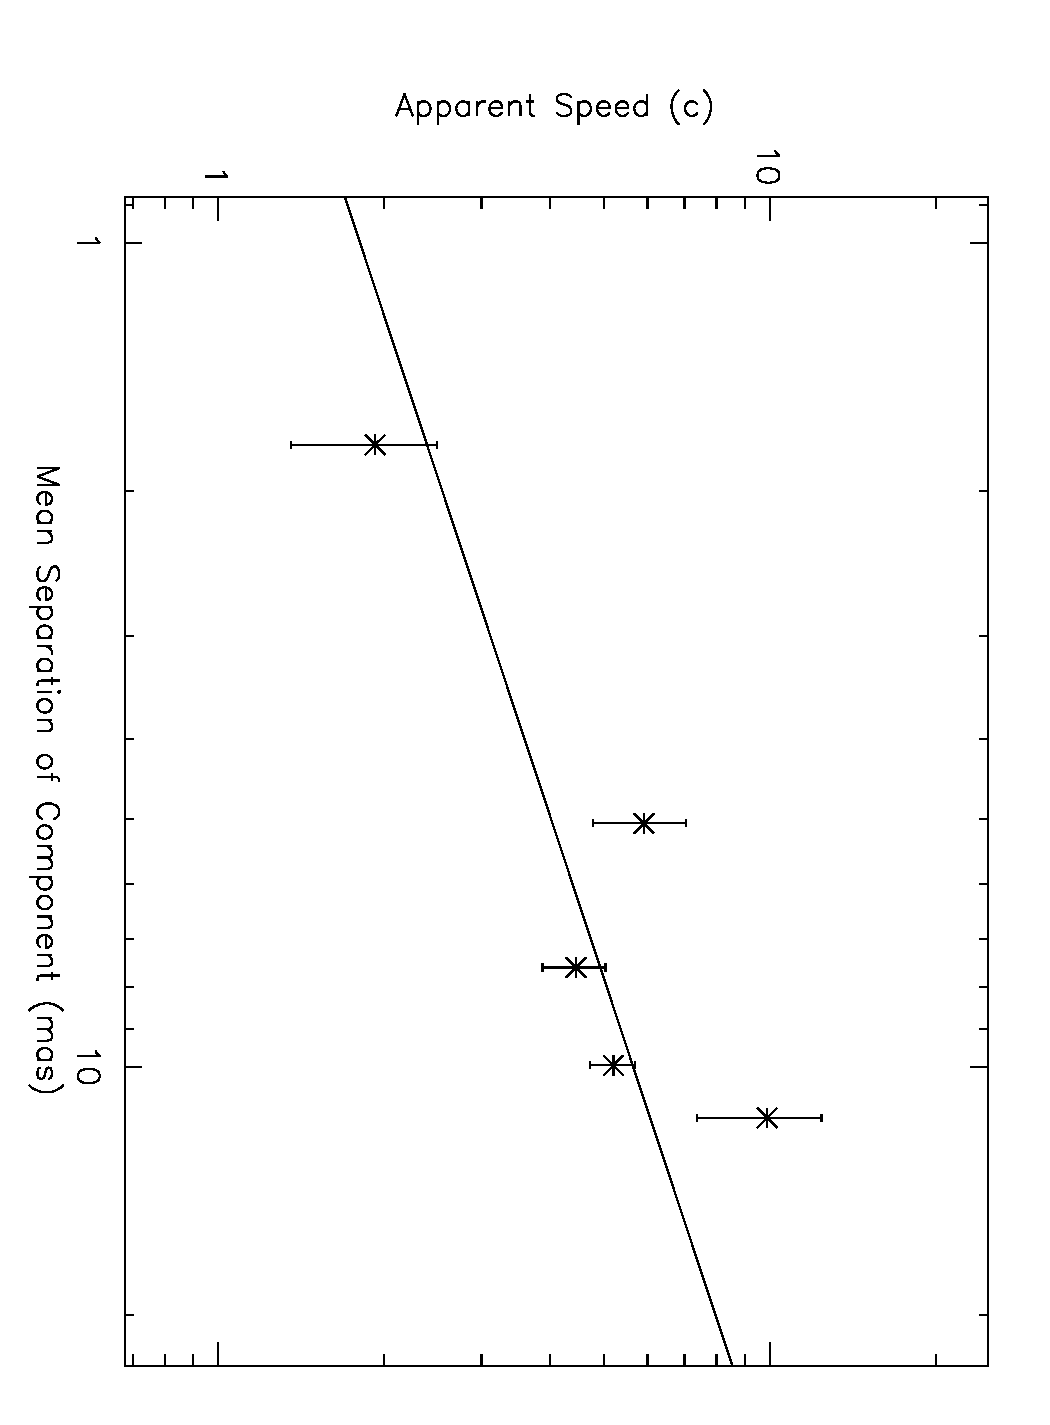
\includegraphics[height=0.7\textwidth,angle=90]{rdv_f6.pdf}
 }
 \caption{Пример линейной подгонки $\ln \beta_\text{app}$ к $\ln\langle{r}\rangle$ для одного из
источников выборки, где $\langle{r}\rangle$~"--- средневзвешенное расстояние компонента, а
$\beta_\text{app}$~"--- его видимая скорость со значениями, взятыми из таблицы 6. Этот пример для
источник 1514\textminus241, с наклоном прямой 0.5, близкий к среднему наклону для всех
подгонок. См. Раздел 4.2 для дальнейшего обсуждения.}
 \label{fig:rdv_beta_app_vs_r}
\end{figure}

\begin{figure}[]
 \centerfloat{
  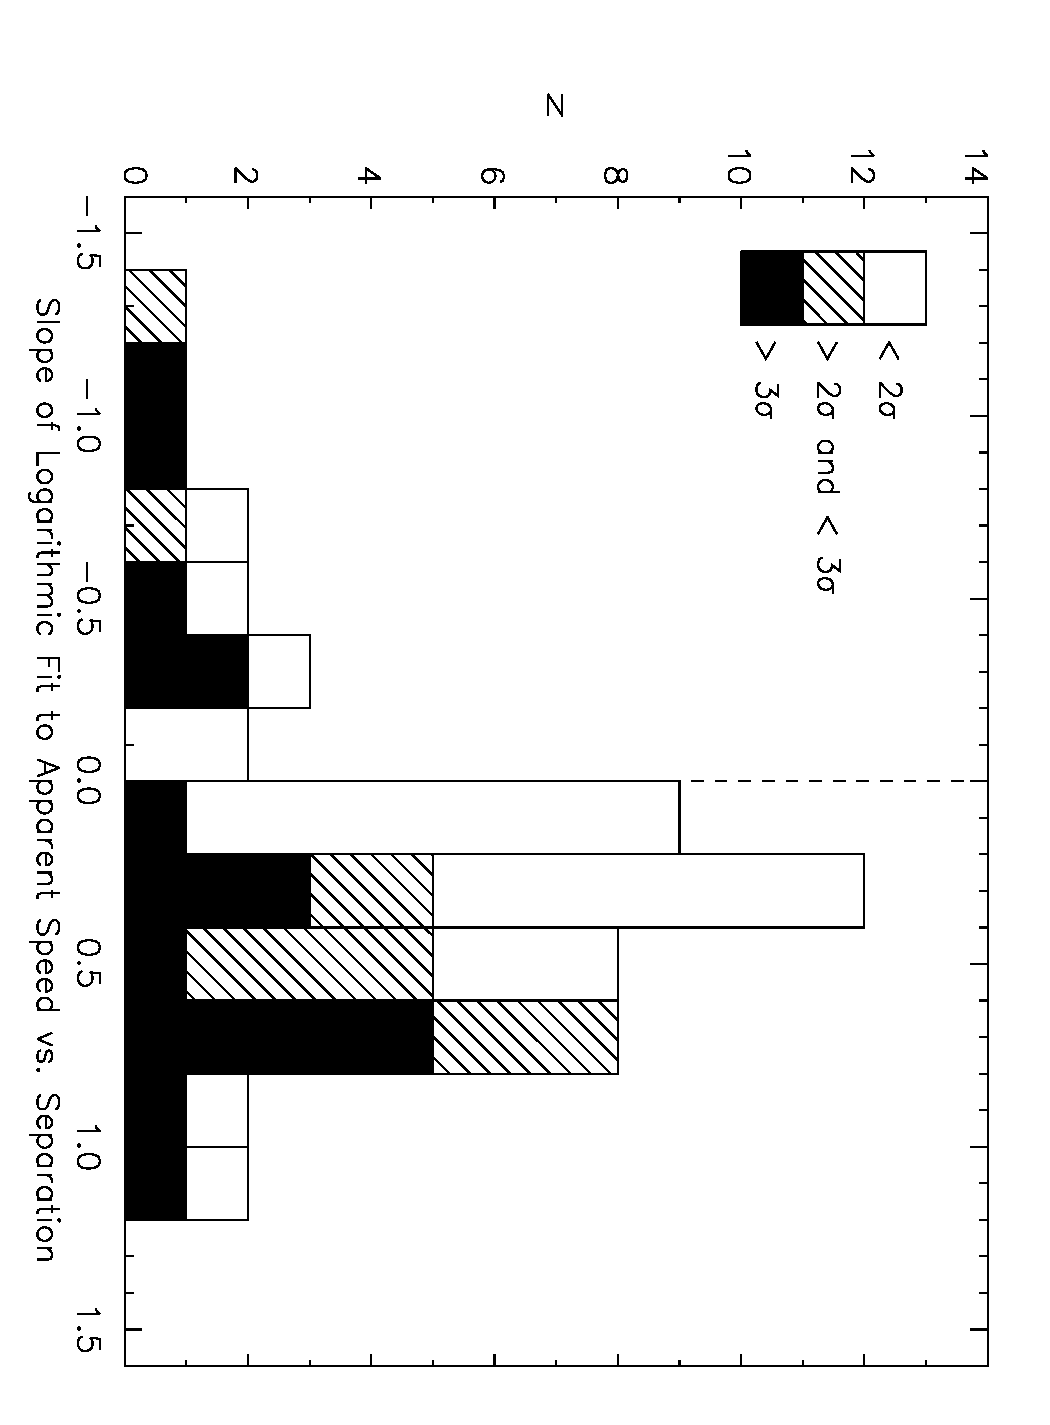
\includegraphics[height=0.7\textwidth,angle=90]{rdv_f7.pdf}
 }
 \caption{Гистограмма наклонов линейных подгонок $\ln \beta_\text{app}$ к $\ln\langle{r}\rangle$ для
отдельных источников, где $\langle{r}\rangle$~"--- средневзвешенное расстояние компонента, а
$\beta_\text{app}$~"--- его видимая скорость со значениями, взятыми из таблицы 6. Постоянное
положительное ускорение вдоль струи даст наклон 0.5. Заштрихованные и закрашенные столбцы указывает
на значимость наклонов на уровнях $2\sigma$--$3\sigma$ и $3\sigma$ соответственно. 3 из 56
источников находятся вне окна гистограммы. См. Раздел 4.2 для дальнейшего обсуждения.}
 \label{fig:rdv_hist_beta_app_vs_r}
\end{figure}

Если струи в обзоре RDV в среднем ускоряются или замедляются, то можно ожидать, что будет
наблюдаться постоянное ощущение изменения измеренных видимых скоростей от компонента к компоненту в
источнике, поскольку компоненты, удаленные от ядра, будут либо систематически быстрее, либо
систематически медленнее, чем компоненты ближе к ядру. Мы исследуем эту связь между кажущейся
скоростью компонентов и средним расстоянием от ядра здесь, а затем исследуем ускоренное движение
отдельных компонентов в Разделе 5. Для каждого из 56 источников в Таблице 6, которые имеют по
крайней мере два нестационарных компонента со значимостью измерении видимой скорости
$\geqslant1\sigma$ мы выполнили подгонку к $\ln \beta_\text{app}$ от $\ln \langle r \rangle$,
используя измеренные значения из таблицы 6 (исключая все кажущиеся скорости со значимостью
$<1\sigma$ и все стационарные компоненты, см. выше). Постоянное положительное видимое ускорение
вдоль струи в источнике дало бы наклон 0.5 для такого фита. На рисунке~\ref{fig:rdv_beta_app_vs_r}
показан пример одной из этих подгонок (для источника 1514\textminus241 с наклоном 0.5, близким к
среднему наклону для всех подгонок), а на рисунке~\ref{fig:rdv_hist_beta_app_vs_r} показана
гистограмма всех 56 наклонов. Для 56 отдельных подгонок 43 дают положительный наклон, а 13 подгонок
дают отрицательный наклон, при этом средний уклон составляет 0.55 (близко к значению 0.5, ожидаемому
для постоянного ускорения в источнике), а медианное значение составляет 0.34. Биномиальная
вероятность измерения 43 положительных уклонов, если они были случайным образом распределены между
положительными и отрицательными значениями, составляет только $P = \num{4e-5}$. Если мы посчитаем
только уклоны, имеющие значимость не менее $2\sigma$, чтобы мы могли быть уверены в знаке, то мы
найдем 22 положительных наклона и 7 отрицательных с биномиальной вероятностью $P = \num{4e-3}$.
Поэтому мы приходим к выводу, что в среднем в нашей выборке компоненты, находящиеся дальше от ядра,
имеют большие кажущиеся скорости, чем компоненты, расположенные ближе к ядру в данном источнике, с
высокой статистической значимостью. Мы обсуждаем связь этого результата с другими результатами в
литературе в разделе 6. Если компоненты дальше от ядра движутся быстрее, чем более близкие
компоненты, то отдельные компоненты должны в среднем испытывать положительные кажущиеся параллельные
ускорения. Мы обсуждаем кажущиеся параллельные ускорения отдельных компонентов в разделе 5.1.

Мы также подтверждаем важный результат, который был также обнаружен в ряде предыдущих исследований
(например, \cite{Lister_2009b,Kellermann_2004,Piner_2007}): что изменение видимых скоростей от
компонента к компоненту в источнике значительно меньше, чем изменение в видимых скоростях от
источника к источнику в выборке. Как и в \cite{Lister_2009b}, мы количественно оцениваем это путем
вычисления стандартного отклонения в измеренных кажущихся скоростях для каждого многокомпонентного
источника. Медиана этих стандартных отклонений составляет $3.1c$; это типичная вариация измеренных
кажущихся скоростей одного источника. Мы также вычисляем среднюю кажущуюся скорость для каждого
источника в выборке и находим, что стандартное отклонение этого набора скоростей составляет $7.6c$;
это типичная вариация кажущейся скорости от источника к источнику в выборке. Это показывает, что
есть характерная физическая скорость, связанная с каждым источником в выборке, которая, вероятно,
является объемной скоростью релятивистского истечения. Затем измеряются отдельные компоненты в
источнике, чтобы иметь относительно небольшой диапазон скоростей относительно этой
характеристической скорости. Если поток ускоряется, то в действительности может существовать
физический диапазон объемных факторов Лоренца внутри источника, который, тем не менее, меньше
диапазона объемных факторов Лоренца от источника к источнику. Компоненты также могут перемещаться в
пределах диапазона коэффициентов Лоренца модели от нуля для стоячего ударной волны, до более высоких
скоростей для <<задних деталей>> (например, \cite{Kadler_2008,Perucho_2008}), вплоть до пикового
объемного Лоренц-фактора истечения. Поскольку нас интересует пиковый объемный Лоренц-фактор,
достигаемый каждой струей за 10-летний период мониторинга, мы и впредь будем использовать самую
быструю наблюдаемую кажущуюся скорость компонента в каждом источнике в качестве измеренной кажущейся
скорости, связанной с этим источником. Это также позволяет проводить прямое сравнение с результатами
MOJAVE, поскольку они также используют самую быструю измеренную кажущуюся скорость в каждом
источнике для характеристики этого источника \cite{Lister_2009b}.

\subsubsection{Изменения скорости между источниками}

\begin{figure}[]
 \centerfloat{
  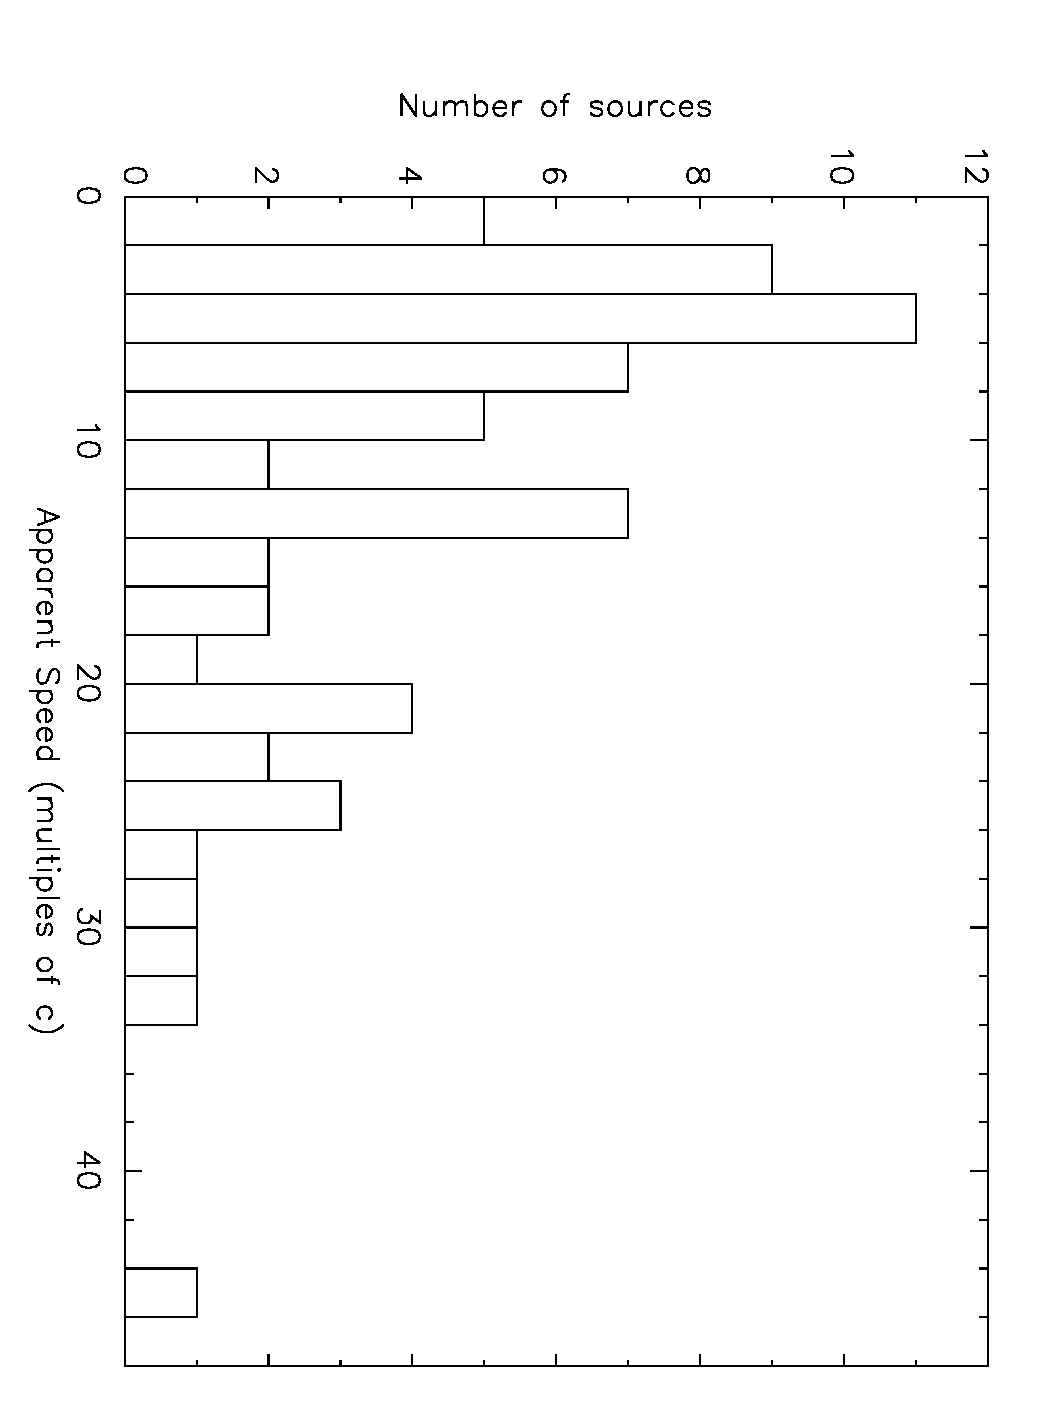
\includegraphics[height=0.7\textwidth,angle=90]{rdv_f8.pdf}
 }
 \caption{Распределение самой быстрой измеренной кажущейся скорости для 65 источников в выборке RDV
с измеренными кажущимися скоростями.}
 \label{fig:rdv_max_speed_dist}
\end{figure}

На рисунке~\ref{fig:rdv_max_speed_dist} показана гистограмма самой быстрой измеренной кажущейся
скорости в каждом источнике из таблицы 6 для всех источников в таблице 6 с измеренным красным
смещением ($N = 65$). Это распределение имеет пик при кажущейся скорости около $5с$, длинный хвост,
простирающийся до максимальной кажущейся скорости $44с$ (для компонента 1 в 1313\textminus333),
средняя кажущаяся скорость $11.5с$, а медианная~"--- $8.3c$. Форма этого распределения аналогична
эквивалентному распределению, измеренному в обзоре MOJAVE \cite{Lister_2009b}, и тест
Колмогорова"--~Смирнова (КС) подтверждает, что между этими двумя распределениями нет существенной
разницы. Однако при сравнении с эквивалентным распределением наибольших видимых скоростей из статьи
\cite{Piner_2007} средняя максимальная кажущаяся скорость увеличилась с $5.9c$ в \cite{Piner_2007}
до $11.5c$ здесь. В \cite{Lister_2009b} также обсуждалось это явление, состоящее в том, что
измерения кажущейся скорости имели тенденцию к увеличению по мере увеличения временного охвата
обзоров от более старых РСДБ обзоров (например, \cite{Britzen_2008,Piner_2007}) до более новых
обзоров, показывая, что высокое угловое разрешение и превосходное временное покрытие могут облегчить
идентификацию быстро движущихся компонентов, которые в противном случае были бы пропущены. В
качестве альтернативы, обнаруженное увеличение самых быстрых скоростей может быть связано с более
длительным периодом наблюдений, который предоставляет больше возможностей для просмотра быстро
движущихся компонентов. Независимо от причины, оба из этих двух недавних обзора кажущихся скоростей
блазаров на более низких частотах (\cite{Lister_2009b} и эта статья) измеряли типичные кажущиеся
скорости, которые аналогичны тем, которые измеряются в исследованиях, проводимых на более высоких
частотах, таких как 43 ГГц ($\sim10c$, например, \cite{Jorstad_2005}).

Поскольку объемный Лоренц-фактор $\Gamma\ge (\beta_\mathrm{app}^{2}+1)^{1/2}$, наблюдаемая пиковая
кажущаяся скорость на рис.~\ref{fig:rdv_max_speed_dist}, равная примерно $44c$, указывает, что
объемные факторы Лоренца в родительской популяции достигают значений, по меньшей мере,
$\Gamma\sim44$. Это максимальное значение также хорошо согласуется с максимальными кажущимися
скоростями, найденными \cite{Jorstad_2005} $46c$ и \cite{Lister_2009b} $51c$. Сужение распределений
кажущейся скорости при более высоких значениях скорости, наблюдаемых на
рисунке~\ref{fig:rdv_max_speed_dist} и в других обзорах, можно воспроизвести при Монте-Карло
моделировании (например, \cite{Lister_1997,Lister_2009b}), предполагая внутреннее степенное
распределение коэффициента Лоренца с наклоном $\sim-1.5$ в популяции блазаров.

\begin{figure}[]
 \centerfloat{
  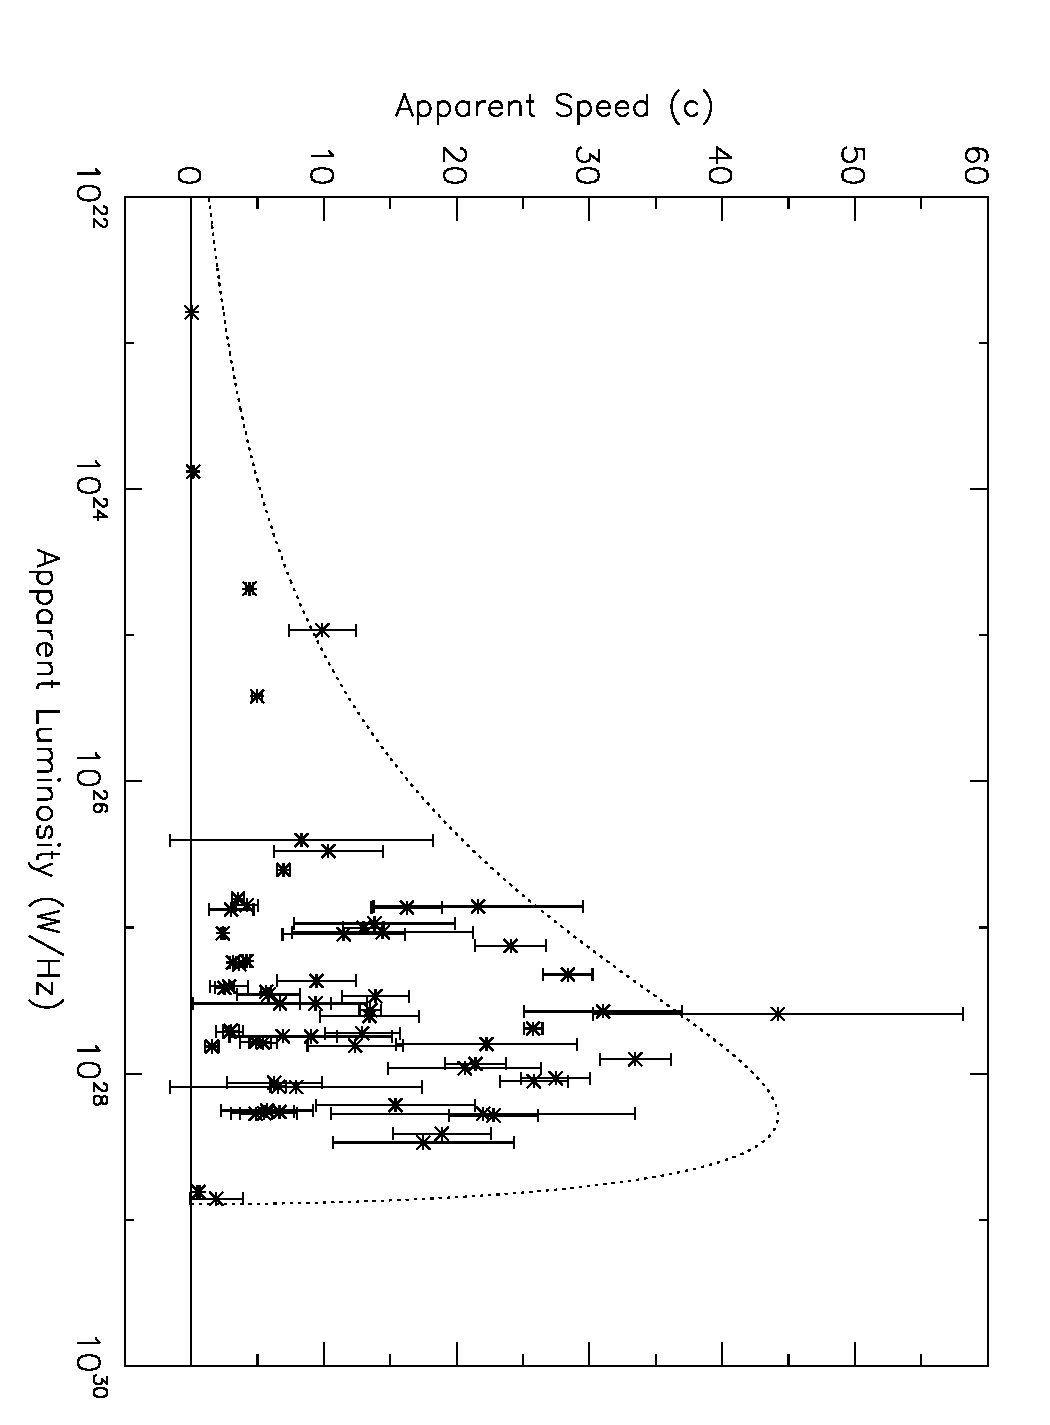
\includegraphics[height=0.7\textwidth,angle=90]{rdv_f9.pdf}
 }
 \caption{Максимальная измеренная видимая скорость в зависимости от медианной видимой светимости
для 65 источников в выборке RDV с измеренными кажущимися скоростями. Пунктирная кривая
соответствует струе с объемным коэффициентом Лоренца 44 и собственной светимостью
\SI{1e25}{\watt\per\hertz}, в зависимости от угла зрения $\theta$, принимая, что доплеровское
усиление пропорционально $\delta^2$, где $\delta$~"--- доплер-фактор.}
 \label{fig:rdv_speed_vs_lum}
\end{figure}

Рисунок~\ref{fig:rdv_speed_vs_lum} показывает самую быструю кажущуюся скорость в каждом источнике в
выборке RDV из Таблицы~6 в зависимости от его медианной видимой РСДБ светимости на 8~ГГц за все
эпохи, использованные в этой статье. Светимости рассчитываются в соответствии с $L=4\pi
D_{l}^{2}S_{8}(1+z)^{-1}$ (с использованием $k$-коррекции с предполагаемым спектральным индексом
$\alpha = 0$), где $D_{l}$~"--- расстояние светимости, а $S_{8}$~"--- медиана общей РСДБ плотности
потока на 8~ГГц. Имеется верхняя граница для распределения, аналогичного тому, которое наблюдается в
обзоре CJF \cite{Vermeulen_1995}, 2-см обзоре \cite{Kellermann_2004} и обзоре MOJAVE
\cite{Lister_2009b}. Как описано в \cite{Cohen_2007}, верхняя огибающая этого распределения выглядит
хорошо согласованной с помощью <<аспектной кривой>>, которая отслеживает единственный источник
заданного объемного фактора Лоренца и внутренней светимости в плоскость $(L, \beta_\text{app})$ по
мере изменения угла обзора $\theta$. Такая аспектная кривая изображена на
рис.~\ref{fig:rdv_speed_vs_lum} для джета с объемным фактором Лоренца, равным 44, и собственной
светимостью \SI{1e25}{\watt\per\hertz}, считая доплеровское усиление как $\delta^{2}$, где $\delta =
1 / (\Gamma (1-\beta \cos \theta))$~"--- доплеровский фактор, а показатель - для гладкой струи
плоского спектра и должен соответствовать основной области \cite{Cohen_2007}. Хотя было показано,
что эта верхняя огибающая не связана с эффектами отбора \cite{Cohen_2007}, ее точное физическое
происхождение неясно; в \cite{Lister_2009b} предполагают, что такая огибающая может возникнуть из-за
внутренней связи между скоростью струи и светимостью в основной популяции, хотя статистика текущих
выборок не может полностью решить эту проблему.

\subsubsection{Гамма-яркие источники}

\begin{figure}[]
 \centerfloat{
  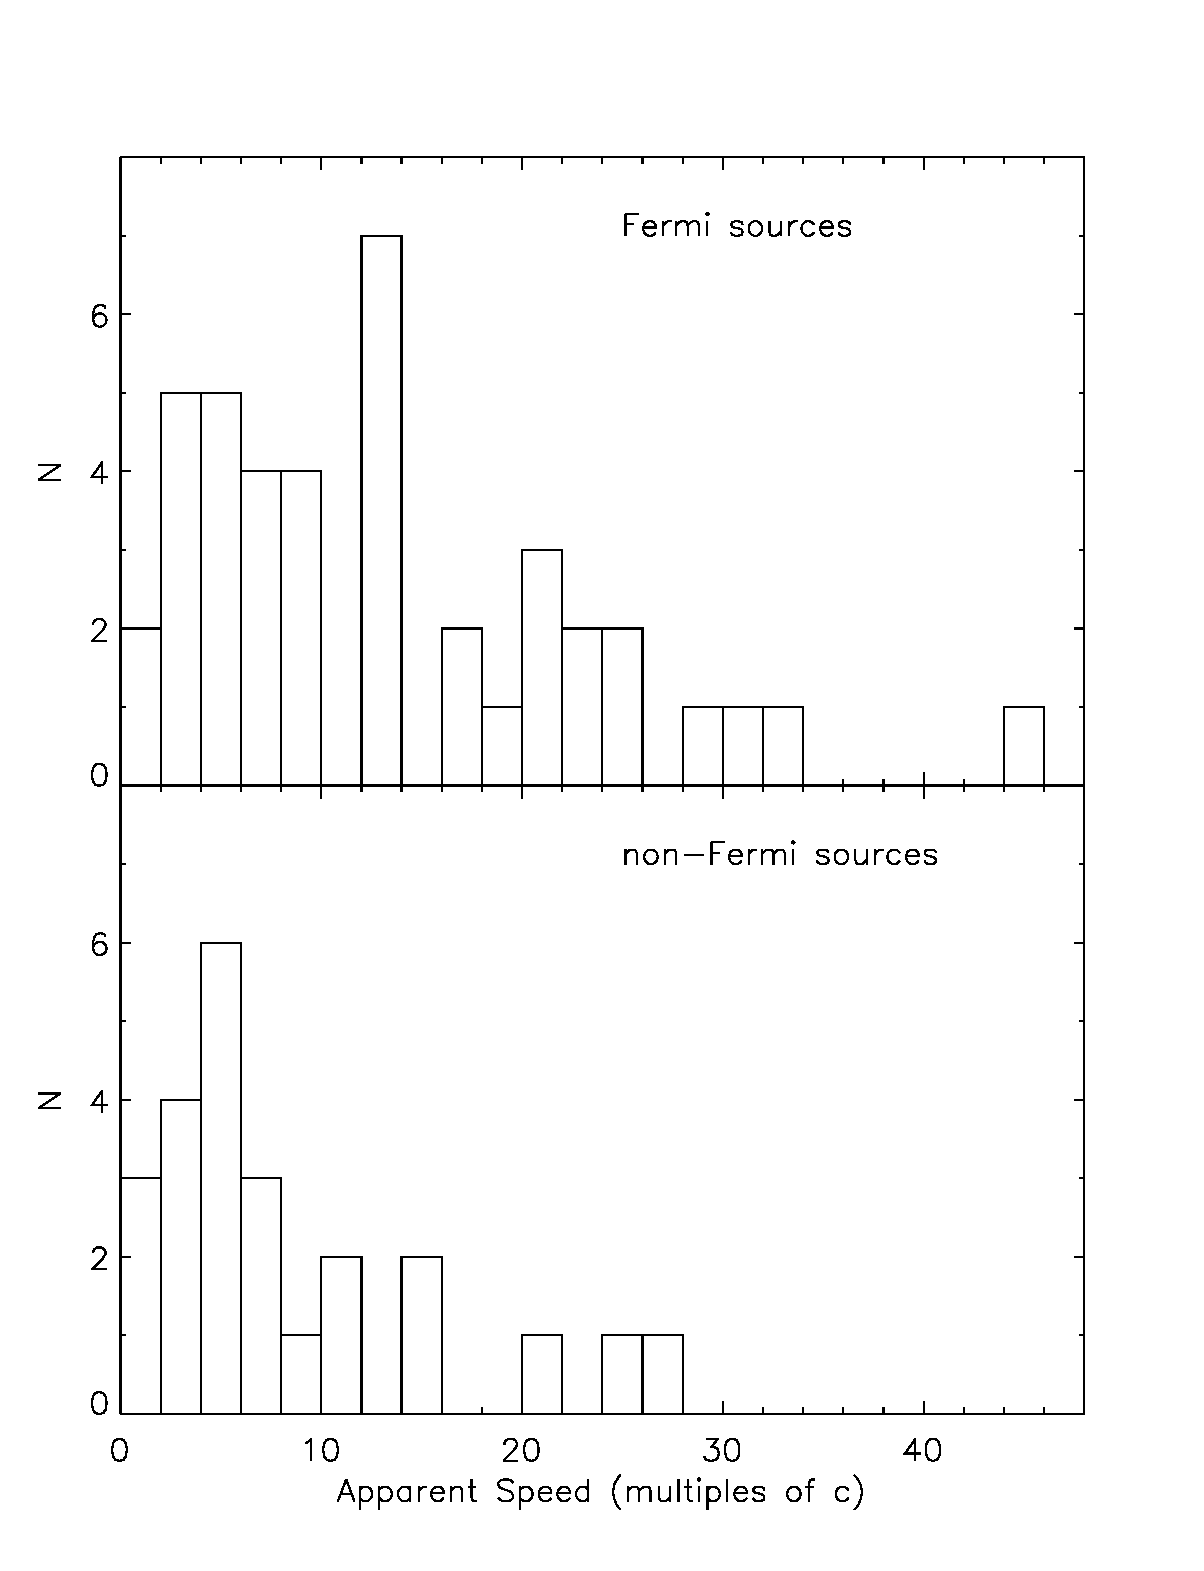
\includegraphics[height=0.5\textheight]{rdv_f10.pdf}
 }
 \caption{Распределение максимальной измеренной видимой скорости для 65 источников на
рисунке~\ref{fig:rdv_max_speed_dist}, для обнаруженных с помощью LAT источники Fermi ($N =
41$, вверху) и не обнаруженных источников ($N = 24$, внизу).}
 \label{fig:rdv_speed_gamma}
\end{figure}

Со времени появления гамма-телескопа EGRET было отмечено, что те источники, которые были обнаружены
в гамма-лучах с энергией ГэВ, имели более быструю видимую скорость, чем источники, которые не были
обнаружены (например, \cite{Jorstad_2001}). Это объясняется тем, что гамма-излучение усиливается за
счет более высокой мощности доплеровского фактора, чем радиоизлучение, поэтому источники
гамма-излучения имеют тенденцию иметь более высокие Лоренц-факторы и меньшие углы обзора
\cite{Pushkarev_2007}, что приводит к на более быстрые кажущиеся скорости (например,
\cite{Lister_1999}). Эта тенденция для более высоких скоростей продолжает отмечаться у блазаров,
обнаруженных с помощью гамма-телескопа Fermi LAT. В \cite{Lister_2009c} обнаружили значительную
разницу в скоростях в источниках обнаруженных и не обнаруженных с помощью LAT в обзоре MOJAVE,
причем обнаруженные LAT источники были быстрее. На рисунке~\ref{fig:rdv_speed_gamma} показано
распределение самых быстрых видимых скоростей в обзоре RDV из таблицы~6, разделенных на LAT
детектированных и недетектированных, из списка детектирований LAT в таблице~\ref{tab:rdv_sources}.
Средняя кажущаяся скорость LAT-обнаруженных источников составляет $12.4c$, в то время как медианная
кажущаяся скорость не обнаруженных источников составляет всего $5.7c$. Эта разница в медиане двух
распределений значима с уровнем достоверности 98.5\,\%, согласно критерию суммы рангов Уилкоксона.
(Для сравнения, t-критерий Стьюдента на разницу в средних значениях, $13.4c$ и $8.3c$, дает значение
97.7\,\%, а непрямой тест КС дает значение 90.7\,\%.) Таким образом, мы подтверждаем что
обнаруженные 2FGL Fermi LAT блазары показывают более высокие видимые скорости, чем необнаруженные
источники в обзоре RDV. Обратите внимание, что ситуация с мощными блазарами, типичными как для
обзора RDV, так и для выборки MOJAVE, которые детектируются на энергиях ГэВ Fermi, контрастирует с
гамма- ТэВ блазарами низкой светимости, которые, как правило, имеют более медленные видимые скорости
на парсековых масштабах по сравнению с радио-отобранными выборками \cite{Piner_2010}. Более подробно
это обсуждается в разделе 6.

Другие свойства радиоизлучения, измеренные в обзоре RDV, помимо кажущейся скорости, также связаны с
состоянием обнаружения LAT Fermi или с измеренным Fermi потоком гамма-излучения. В
\cite{Kovalev_2009a} показана корреляция между неодновременной РСДБ плотностью потока на 8~ГГц,
включая данные обзора RDV, и потоком гамма-излучения Fermi. В \cite{Kovalev_2009a} также показано,
что обнаруженные LAT источники имеют более высокие плотности РСДБ потока на 8~ГГц по сравнению с
необнаруженными источниками. \cite{Pushkarev_Kovalev_2012} используют подвыборку из 370 источников
из 19
экспериментов RDV в таблице~\ref{tab:rdv_obstab} между 1998 и 2003 годами, чтобы показать, что
источники, обнаруженные с помощью LAT, имеют более высокие плотности потока РСДБ ядра и яркостные
температуры на 8 и 2~ГГц, и более плоские спектральные индексы в джетах между 8 и 2~ГГц по сравнению
с необнаруженными источниками. Несмотря на эти существенные корреляции потока из данных RDV, такие
сравнения лучше всего проводить с квазиодновременными данными потока из-за переменной природы
источников. Такие исследования были выполнены для квази-одновременных данных VLBA и Fermi из обзора
MOJAVE, например, \cite{Kovalev_2009b,Pushkarev_2010,Lister_2011}.

\subsection{Обсуждение}

В предыдущих разделах этой статьи мы представили кинематический анализ большой выборки данных VLBI
из серии экспериментов RDV. Мы пришли к выводу, что этот анализ показывает статистически значимые
доказательства положительного ускорения струи на парсековых-масштабах на этой выборке струй
струи на основе двух взаимно согласованных линий доказательств. Это наблюдение о том, что
компоненты, находящиеся дальше от ядра, имеют тенденцию появляться быстрее, чем компоненты,
расположенные ближе к ядру, в большинстве струй в выборке (раздел 4.2), и что отдельные компоненты,
как правило, имеют ускорения, которые увеличивают их кажущиеся скорости (раздел 5.1). Здесь мы
связываем эти наблюдения с другими результатами в литературе и с физическими свойствами источников.

Другие многоструйные исследования также показали тенденцию, более удаленные компоненты
струи быстрее, чем компоненты, расположенные ближе к ядру в том же объекте (например,
\cite{Homan_2001,Piner_2006,Britzen_2008}). В \cite{Homan_2001} наблюдали этот эффект в пяти из
шести источников (из их выборки из 12), которые имели несколько компонентов с измеримым собственным
движением; это было также отмечено во всех трех высокоскоростных блазарах, изученных
\cite{Piner_2006}. Наиболее существенно, в \cite{Britzen_2008} выполнены подгонки
$\beta_\text{app}$ к $r$ для 105 источников из 293 в обзоре CJF; эти подгонки аналогичны нашим
подгонкам к тем же двум величинам, описанным в разделе 4.2. На основании этих подгонок они пришли к
выводу, что существует небольшая тенденция к положительному ускорению; однако их результаты были
несколько затруднены наличием только трех эпох на источник и более низким угловым разрешением.

Существует очевидное противоречие с этими наблюдениями, которое также было отмечено: что в более
старых РСДБ исследованиях, проводимых на более низких частотах (и, следовательно, с более низким
разрешением и, следовательно, с наблюдением компонентов дальше от ядра), наблюдаемые скорости имели
тенденцию быть ниже по сравнению с исследованиями сделано на более высоких частотах (и,
следовательно, в более высоких разрешениях, и наблюдение компонентов ближе к ядру). Например,
кажущиеся скорости, измеренные в обзоре CJF \cite{Britzen_2008} на частоте 5 ГГц были в среднем
медленнее, чем в 2 см обзоре на частоте 15 ГГц \cite{Kellermann_2004}, которая, в свою очередь,
была медленнее, чем в обзоре блазаров EGRET на 22 и 43 ГГц \cite{Jorstad_2001}. Казалось, это
означало, что компоненты были быстрее ближе к ядру. Однако, как обсуждалось в Разделе 4.3, в более
новых РСДБ исследованиях, которые намного лучше сэмплированны по времени как на более низких, так и
на более высоких частотах, большая часть этого очевидного различия исчезла. Улучшение временного
охвата в новых обзорах может помочь в выявлении быстро движущихся компонентов, пропущенных в
предыдущих обзорах. Как мы отмечали в Разделе 4.3, исследования видимых скоростей блазаров на 15
ГГц и на 8 ГГц в \cite{Lister_2009b} и в этой статье в настоящее время измеряют типичные кажущиеся
скорости, которые аналогичны измеренным на более высоких частотах ($\sim10c$, например,
\cite{Jorstad_2005}). В любом случае, поскольку эти разные выборки были выбраны на основе разных
физических характеристик, некоторые по их радиоизлучению, а некоторые по их гамма-излучению,
некоторые различия в скоростях струи между выборками не удивительны и не обязательно обусловлены
расстоянием компонентов от ядра.

В разделе 5.1 мы сообщили результаты по измеренным кажущимся параллельным ускорениям отдельных
компонентов струи. Мы обнаружили, что параллельные ускорения были значительно больше, чем
перпендикулярные ускорения, показывая, что в параллельных ускорениях преобладают изменения фактора
Лоренца, а не изгиб струи. Среди параллельных ускорений положительные ускорения преобладали над
отрицательными ускорениями. Средние относительные параллельные ускорения были в диапазоне 0.1--0.2
в год, в зависимости от подвыборки. Чтобы связать эти наблюдаемые кажущиеся ускорения с изменениями
внутренних свойств источника, отметим, что если кажущиеся параллельные ускорения целиком связаны с
изменениями фактора Лоренца, то наблюдаемое относительное параллельное ускорение определяется как
\begin{equation}
\dot{\eta}_{\parallel}\equiv\frac{\dot{\beta}_\mathrm{\parallel app}}{\beta_\mathrm{app}}\approx
\frac{\dot{\Gamma}}{\Gamma}\delta^{2}.
\end{equation}
Этот результат может быть получен путем дифференцирования уравнения (\ref{speedeqn}) по времени в
системе отсчета наблюдателя с постоянной $\theta$, см. также обсуждение этого уравнения в
\cite{Homan_2009}. Итак, $\dot{\Gamma}/\Gamma\approx\dot{\eta}_{\parallel}/\delta^{2}$, и с
типичными наблюдаемыми кажущимися скоростями 10$c$ мы имеем в терминах порядков величин $\delta\sim
10$ и $\dot{\eta}_{\parallel}\sim $\SI{0.1}{\per\year}, для
$\dot{\Gamma}/\Gamma\sim$\SI{1e-3}{\per\year} в системе отсчета хозяйской галактики.
Типичное расстояние компонента от ядра в обзоре RDV составляет около 10 парсек (projected),
или около 100 парсек de-projected. Таким образом, типичный компонент в обзоре RDV имеет
$\dot{\Gamma}/\Gamma\sim$\SI{1e-3}{\per\year} в системе отсчета галактики-хозяина, в $\sim100$
парсек от ядра. Это тот же порядок величины собственных ускорений, который обнаружен в обзоре
MOJAVE \cite{Homan_2009}. Собственные изменения фактора Лоренца, соответствующие наблюдаемым
ускорениям, относительно скромны. Такой уровень собственного ускорения, если он постоянен,
недостаточен для получения высоких факторов Лоренца, которые наблюдаются на этих расстояниях от
ядра. Собственное ускорение должно быть как минимум на порядок больше ближе к ядру, чтобы получить
большие объемные коэффициенты Лоренца, которые наблюдаются на этих расстояниях. Поэтому типичный
компонент должен быть ускорен до $\Gamma\sim10$ к тому времени, когда он достигает расстояний в
$\sim10 $ парсек от ядра (de-projected). Дальше этих расстояний существуют типичные
ускорения $\dot{\Gamma}/\Gamma\sim$\SI{1e-3}{\per\year}, которые соответствуют
примерно еще 30\,\% увеличению фактора Лоренца на $\sim 100$ парсек от ядра
(de-projected). Дальше ускорение должно уменьшаться (или даже становиться отрицательным,
как это наблюдалось в \cite{Homan_2009}) на килопарсековых масштабах.

Эти наблюдения положительных ускорений в масштабе парсек согласуются с существованием расширенной
области магнитного ускорения, подобной той, которая была предложена \cite{Vlahakis_2004}. Эти
авторы утверждают, что магнитное ускорение должно все еще быть активным на масштабах парсек, а
также утверждают, что некоторые ранее наблюдавшиеся расширенные ускорения вряд ли имели чисто
гидродинамическое (немагнитное) происхождение. Однако другие модели магнитного ускорения (например,
\cite{Granot_2011,McKinney_2006}) предсказывают, что ускорение должно почти закончится примерно на
0.1 пк от центральной машины. Есть также несколько других аргументов, что преобразование
магнитной в кинетическую энергию должно почти завершиться на парсековых масштабах. Вспышечная
активность, наблюдаемая в ядрах блазаров, показывает, что в этом месте струи уже преобладает
вещество, если вспышки происходят из-за внутренних ударов. Однако если такая вспышечная активность
вместо этого связана с диссипацией магнитной энергии, а не с внутренними ударами, тогда струя с
доминированием вещества может не потребоваться (например, \cite{Giannios_2011,Sikora_2005}). Следуя
другому аргументу, \cite{Celotti_2008} пришли к выводу, что в струях мощных блазаров
доминирует вещество на масштабах парсек посредством SED-моделирования излучающих областей. Хотя
наблюдения, приведенные в этой статье, показывают, что на парсековых масштабах наблюдаются умеренные
ускорения, сами по себе они не могут различить магнитную или гидродинамическую причину этих
ускорений. Кроме того, так как мы наблюдаем движения центроидов яркости в потоке, мы не можем
сбрасывать со счетов возможность модели, а не объемных ускорений для любого отдельного компонента.
Обратите внимание, что объемные ускорения должны также приводить к изменениям плотности потока
компонентов за счет изменения доплеровского усиления, но, поскольку такие изменения будут сочетаться
с собственными изменениями плотности потока, будет трудно использовать это в качестве диагностики на
практике. Однако преобладание положительных параллельных ускорений над отрицательными предполагает
наличие связи с физическими свойствами струи, такими как скорость объемного потока, а не с
движениями случайных структур.

Разница между результатами ускорения, представленными здесь, и результатами, представленными в
обзоре MOJAVE \cite{Homan_2009}, заключается в том, что в то время как в обзоре RDV преобладают
положительные параллельные ускорения, \cite{Homan_2009} обнаружил примерно равное количество
положительных и отрицательных параллельных ускорений с переходом от положительного к отрицательному
ускорению происходящих на расстоянии около \SI{15}{\parsec} от ядра (в проекции). Как видно из
рисунка 14, поскольку мы изучили меньшее количество компонентов релятивистских струй, чем MOJAVE
(см. таблицу~\ref{tab:rdv_comptab}), после применения различных обрезаний по качеству у нас не
осталось достаточно компонентов со значительными ускорениями при $>$\SI{15}{\parsec} (в проекции) от
ядра, чтобы сделать убедительное утверждение об этой области струи. Тем не менее, в пределах
\SI{15}{\parsec} (в проекции) от ядра, мы убедительно продемонстрировали, что компоненты струи
имеют тенденцию к положительному параллельному ускорению: 16 из 19 компонентов на рисунке 14 в
пределах \SI{15}{\parsec} (в проекции) от ядра имеют положительное ускорение. Это согласуется с
результатами \cite{Homan_2009} для этой области струи. Мы также отмечаем, что \cite{Jorstad_2005}
находят аналогичное смещение для положительных параллельных ускорений в исследовании, в котором
предпочтение отдается компонентам в пределах \SI{15}{\parsec} (в проекции) от ядра из-за высокой
частоты наблюдения. Таким образом, мы интерпретируем результаты обзора RDV, \cite{Homan_2009} и
\cite{Jorstad_2005}, как взаимно согласованные с тем, что Лоренц-фактор компонентов струи в
мощных блазарах имеют тенденцию к увеличению во всей области внутренней части струи до
\SI{15}{\parsec} (в проекции) от ядра.

Наконец, мы также хотим подчеркнуть различие между выборкой мощных блазаров, изученной в этой
статье и в \cite{Piner_2007}, и выборкой менее мощных ТэВ-блазаров, изученным, например, в
\cite{Piner_2010}. Получены существенные доказательства, указывающие на существенное замедление
потока до масштабов парсек, наблюдаемых с помощью РСДБ в близких ТэВ-источниках с низкой мощностью,
в отличие от небольшого общего положительного ускорения, которое было измерено в этой статье для
выборки источников большой мощности. Такое значительное различие между масштабами ускорения и
замедления для источников высокой и низкой мощности, вероятно, связано с фундаментальными различиями
между центральным машинами и/или средой в этих двух классах источников.

\subsection{Выводы}

Мы изучили кинематику на порсековых масштабах в выборке из 68 внегалактических струй, используя
глобальные РСДБ наблюдения на частоте 8 ГГц из серии экспериментов RDV, значительно расширяя наше
предыдущее такое исследование из \cite{Piner_2007}. Мы включили в это исследование все источники,
которые наблюдались в 20 или больше эпохах в течение серии из 50 РСДБ экспериментов с 1994 по
2003 год. Мы создали и проанализировали 2753 РСДБ изображения из этих экспериментов, со средним
значением 43 эпохи наблюдения на источник. С точки зрения углового разрешения и временного охвата
этот обзор RDV аналогичен обзору MOJAVE \cite{Lister_2009b,Homan_2009}. Мы подгоняем гауссовы
модели к функции видности, связанной с каждым изображением, и определили в общей сложности 225
компонентов струи в 66 источниках, которые можно проследить от эпохи к эпохе. Полиномы второго
порядка подгонялись к $x(t)$ и $y(t)$ для каждого компонента, чтобы изучить его скорость и
ускорение. Результаты наблюдений, связанные с измеренными кажущимися скоростями, можно суммировать
следующим образом:
\begin{enumerate}
 \item
 Когда в струе присутствует несколько движущихся компонентов, компоненты, находящиеся дальше от
ядра, имеют тенденцию (примерно в 75\,\% времени) иметь большую кажущуюся скорость, чем компоненты,
расположенные ближе к ядру, с высокой статистической значимостью.

\item
 Изменение видимых скоростей от компонента к компоненту в источнике значительно меньше, чем
изменение видимых скоростей от источника к источнику в выборке, что свидетельствует о наличии
характерной скорости, связанной с каждым источником.

\item
Распределение самых быстрых измеренных видимых скоростей в каждом источнике показывает максимум
44$c$ и медиану 8.3$c$.

\item
Источники, обнаруженные с помощью гамма-телескопа Fermi LAT, показывают более высокие кажущиеся
скорости со средним значением $12.4с$, чем те, которые не были обнаружены, со средним значением
$5.7с$.

\item
Стационарные или медленно движущиеся компоненты найдены в 19 источниках. Эти компоненты
сгруппированы в $\sim$\SI{4}{\parsec} (в проекции) от ядра, и могут представлять действительно
стационарные особенности, такие как реколлимационные шоки.
\end{enumerate}

Мы определили высококачественные подвыборки полного набора из 225 компонентов для анализа ускорения,
и для каждого из этих компонентов мы проанализировали относительное ускорение, параллельное и
перпендикулярное направлению вектора средней скорости, а также разницу между направлением вектор
средней скорости и средневзвешенный угол положения. Результаты наблюдений, связанные с измеренными
ускорениями и нерадиальными движениями, можно суммировать следующим образом:
\begin{enumerate}
 \item
 Значительное нерадиальное движение является обычным явлением, возникающим примерно у половины
компонентов, имеющих значимость $\ge2\sigma$. Когда происходит не радиальное движение, оно
стремится выровнять компонент с расположенной ниже структурой струи.

\item
<<Высокие>> относительные ускорения (величины, которые по крайней мере на $2\sigma$ выше
0.1~год$^{-1}$) довольно распространены и составляют около 1/4 параллельных ускорений и 1/7
перпендикулярных ускорений, такие же показатели высоких ускорений были обнаружены в обзоре MOJAVE
(\cite{Homan_2009}).

\item
Распределения относительных параллельных и перпендикулярных ускорений статистически различны, причем
параллельные ускорения имеют большую среднюю величину примерно в 1.7 раза. Это различие
подразумевает, что существуют внутренние изменения в Лоренц-факторов компонентов, которые
доминируют над изгибом струи при создании наблюдаемых параллельных ускорений.

\item
Положительные параллельные ускорения статистически преобладают над отрицательными параллельными
ускорениями. Средневзвешенное относительное параллельное ускорение для 64-компонентной подвыборки
составляет \SI{0.133+-0.014}{\per\year}. Типичное наблюдаемое относительное параллельное
ускорение, равное 0.1~год$^{-1}$, соответствует увеличению фактора Лоренца в объеме или
структуре в системе отсчета хозяйской галактики порядка $\dot{\Gamma} / \Gamma
\sim10^{-3}$~год$^{-1}$ на расстоянии порядка 100 парсек (de-projected) от ядра.

\end{enumerate}

Таким образом, каждая из струй блазаров имеет характерную скорость в пределах примерно 100 пк
(de-projected) от сверхмассивной черной дыры, причем любое боковое движение имеет тенденцию
перемещать компоненты вниз по каналу в направлении предыдущего компонента. Средний компонент
увеличивает свою кажущуюся скорость с наблюдаемым темпом около 10\,\% в год на расстояниях около
100 пк (de-projected) от ядра. Это кажущееся ускорение соответствует увеличению фактора Лоренца
со скоростью примерно одна часть в $10^3$лет$^{-1}$ в системе отсчета хозяйской галактики. Меньшая
часть компонентов имеет видимое замедление на этих расстояниях.

Все приведенные выше выводы носят статистический характер и не обязательно применимы к
какому-либо конкретному источнику. Принимая во внимание результаты аналогичного исследования
кинематики в MOJAVE \cite{Homan_2009}, результаты ускорения, представленные здесь, показывают, что
умеренные изменения в объемных или типовых коэффициентах Лоренца в масштабах парсек являются
относительно распространенной особенностью релятивистских струй. Этот результат наблюдений в
настоящее время подтвержден взаимно непротиворечивым образом с высокой статистической значимостью
двумя крупными РСДБ обзорами (хотя следует отметить, что эти два обзора не являются
полностью статистически независимыми, поскольку у них 37 общих источников). Эти наблюдения
согласуются со скромным увеличением объемной кинетической энергии на парековых масштабах, хотя
источник этой энергии не определяется из этих наблюдений.

Эта статья и \cite{Piner_2007} представляют верхушку айсберга астрофизики, которую можно сделать с
помощью данных RDV. На сегодняшний день проведено около 100 экспериментов, и общее количество
потенциальных изображений составляет около 10000 на частотах 8 и 2 ГГц. Например, добавление к этому
исследованию экспериментов, которые наблюдались с 2003 года, может удвоить размер
кинематического обзора, представленного здесь. Кроме кинематики могут быть изучены многие вещи, в
том числе изменчивость потока и многоволновые корреляции, спектральный индекс и непрозрачность
ядра (например, \cite{Kovalev_2008,Pushkarev_Kovalev_2012}), хребтовые линии и изгиб струй, а
также поперечные структуры в струях.


\section{RADIOASTRON OBSERVATIONS OF THE QUASAR 3C273:
A CHALLENGE TO THE BRIGHTNESS TEMPERATURE LIMIT}

\subsection{Введение}

Открытие полвека назад переменности плотности потока радиоизлучения квазаров на временных
масштабах, всего несколько месяцев \cite{Sholomitsky_1965a,Sholomitsky_1965b,Dent_1965}, показало,
что линейные размеры равны световым месяцам, что соответствует угловым размерам порядка одной
угловой миллисекунды или менее и предполагают необычайно высокие видимые яркостные температуры
\cite{Pauliny_Toth_1066}. Последующее открытие с использованием радиоинтерферометрии со
сверхдлинными базами (РСДБ) сверхсветового движения и релятивистского излучения с доплеровскими
факторами $\delta \sim 10$ (например, \cite{Lister_2013}), по-видимому, объясняет экстремальные
значения видимого размера и яркостной температуры, полученной из внутренней переменности
\cite{Kellermann_1981}.  Для некогерентного синхротронного излучения релятивистских
электронов в отсутствие релятивистского бустинга максимальная яркостная температура
ограничивается обратным комптоновским охлаждением примерно до \SI{e11.5}{\kelvin}
(\cite{Kellermann_1969,Readhead_1994})  или \SI{5e10}{\kelvin} в случае равнораспределения между
энергий частиц и магнитного поля \cite{Readhead_1994}. Релятивистское усиление может увеличить
наблюдаемую яркостную температуру, $T_\text{obs} = \delta \times T_\text{int}$ на доплеровский
коэффициент $\delta = (1 - \beta^2)^{1/2} (1 - \beta \cos\phi)^{-1}$, где $T_\text{int}$~"---
внутренняя яркостная температура, $\beta = v/c$~"--- скорость струи в единицах скорости света, а
$\phi$~"--- угол между вектором скорости струи и лучом зрения. Кажущаяся скорость струи
$\beta_\text{app} = \beta \sin \phi (1 - \beta \cos \phi)^{-1}$.

Тем не менее, наблюдения межзвездной сцинтилляции во многих источниках с плоским спектром (например,
\cite{Lovell_2008}), отражающие очень малые угловые размеры и очень высокие яркостные температуры, а
также быстрое изменение излучения ТэВ от некоторых квазаров \cite{Hinton_2009}, предполагают
либо значительно более высокие Доплер-факторы, чем те, которые были оценены из РСДБ наблюдений
по кинематике квазаров \cite{Lister_2013}, либо, возможно, другой механизм излучения, чем
некогерентное синхротронное излучение релятивистских электронов (например,
\cite{Blandford_Konigl_1979}). Предыдущие наземные \cite{Kovalev_2005,Lee_2008} и
космические \cite{Frey_2000,Tingay_2001,Dodson_2008} РСДБ (SVLBI) наблюдения
согласуются с ожидаемыми малые размеры и высокими наблюдаемыми яркостными температурами квазаров,
выведенные из их собственной переменности, а также с пределами, обсужденными выше. Однако
предыдущие РСДБ измерения не могли достичь длины базы или углового разрешения, необходимого для
окончательного решения вопроса о высокой яркостной температуре.

С запуском 18 июля 2011 года Федеральным космическим агентством России космического радиотелескопа
(КРТ) <<РадиоАстрон>> появилась возможность напрямую проверить режим чрезвычайно
высокой видимой яркостной температуры. Спутник <<Спектр-Р>> находится на девятидневной
высокоэллиптической орбите Земли с переменным апогеем до 350\,000\,км. Он оснащен 10-метровым
параболическим радиотелескопом и работает на частотах 330 МГц (92 см), 1.7 ГГц (18 см), 4.8 ГГц
(6.2 см) и 22 ГГц (1.3 см) \cite{Kardashev_2013_rus}.

\begin{figure*}[]
\centerfloat{
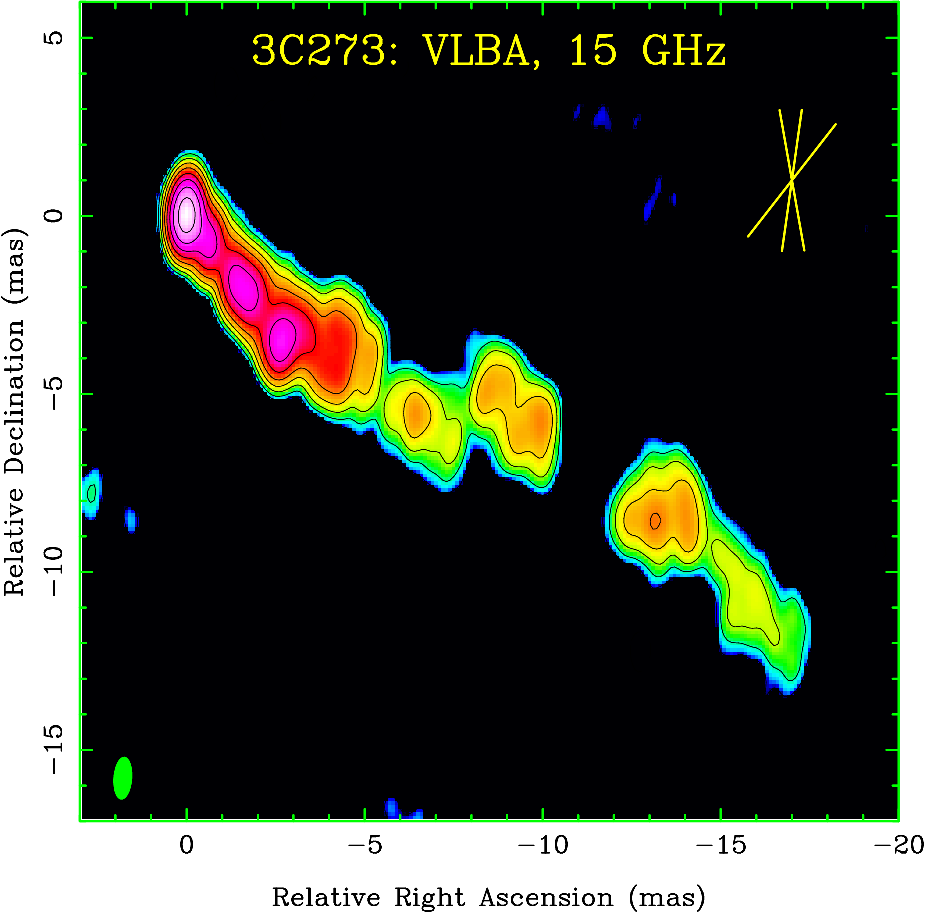
\includegraphics[width=0.39\textwidth,trim = 0cm 0cm 0cm 0cm]{3C273_VLBA_Uband.pdf}
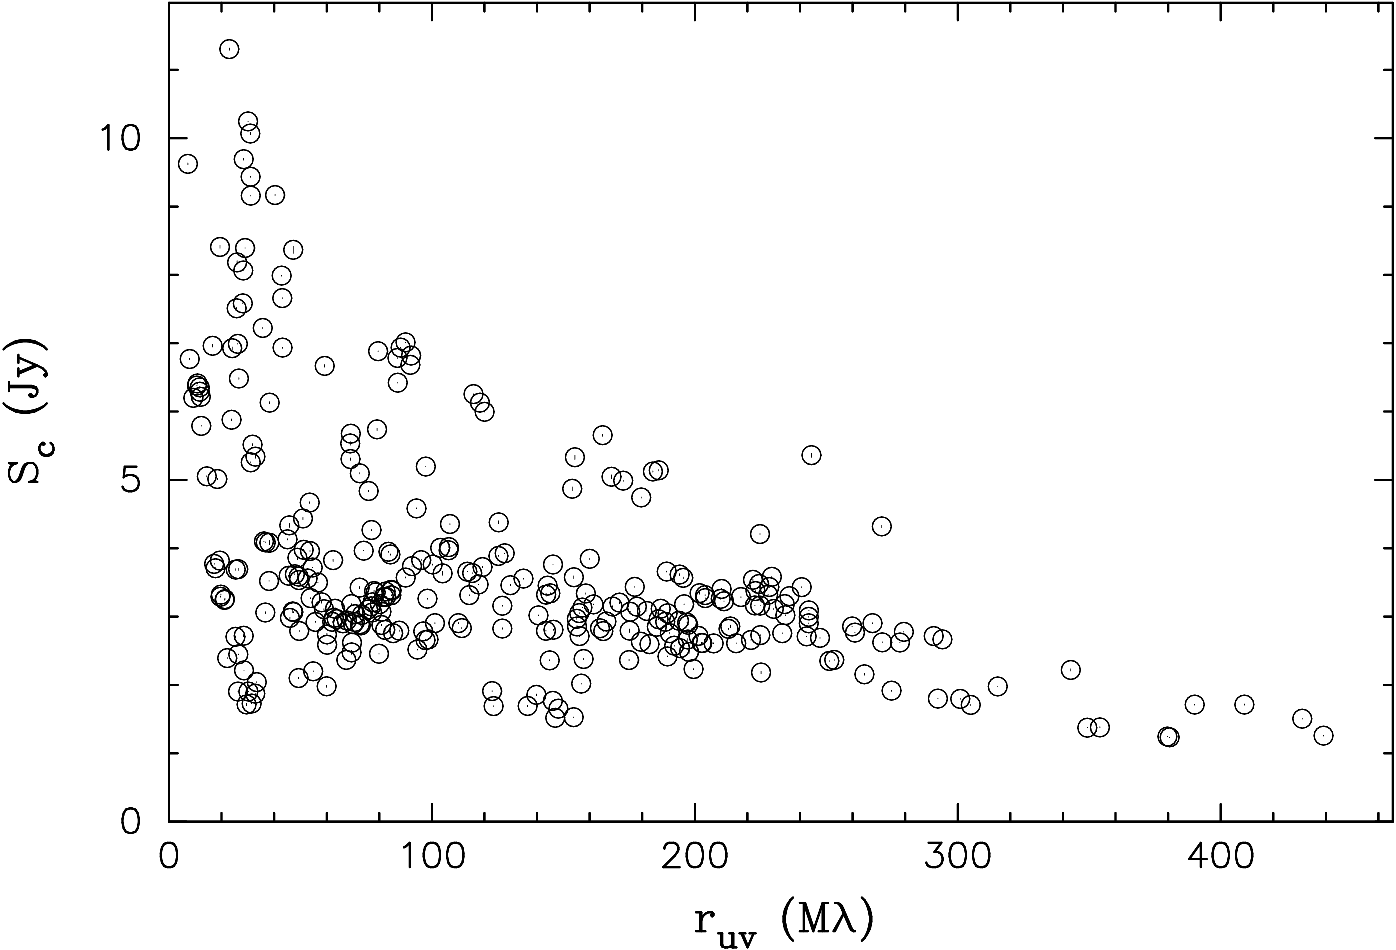
\includegraphics[width=0.56\textwidth,trim = -0.1cm 0cm 0cm 0cm]{1226+023_U_2013_02_10_yyk_rad.pdf}
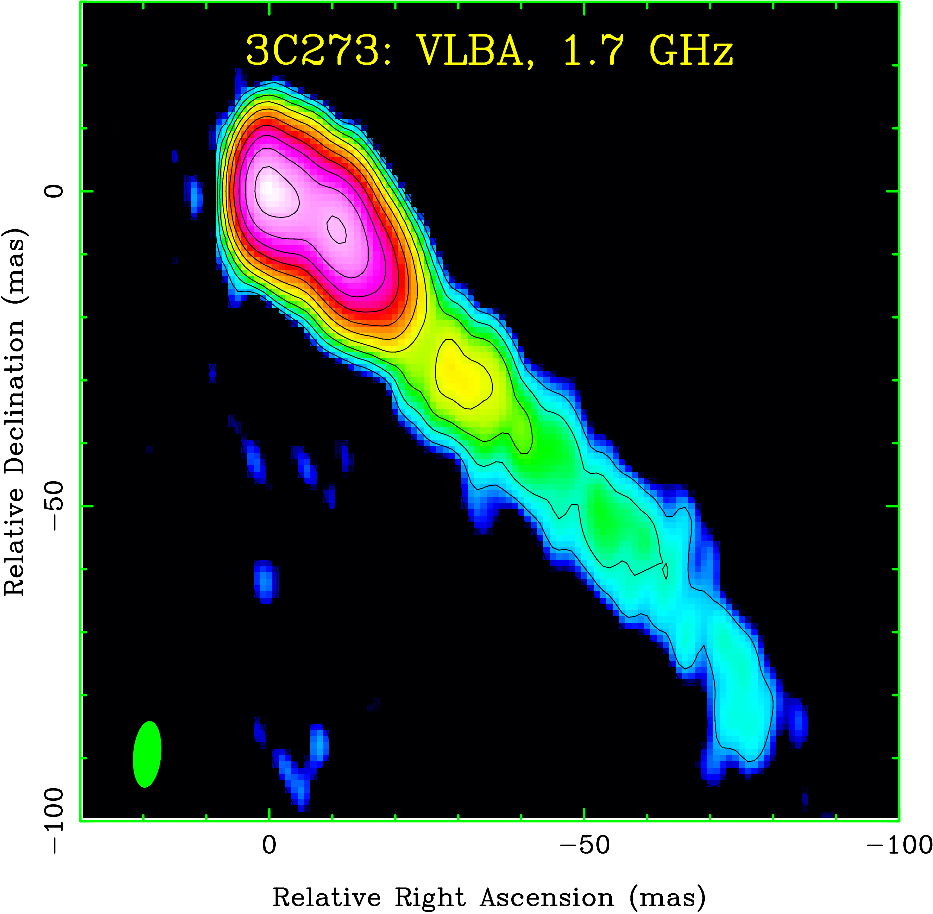
\includegraphics[width=0.39\textwidth,trim = 0cm 0cm 0cm -1cm]{3C273_VLBA_Lband.pdf}
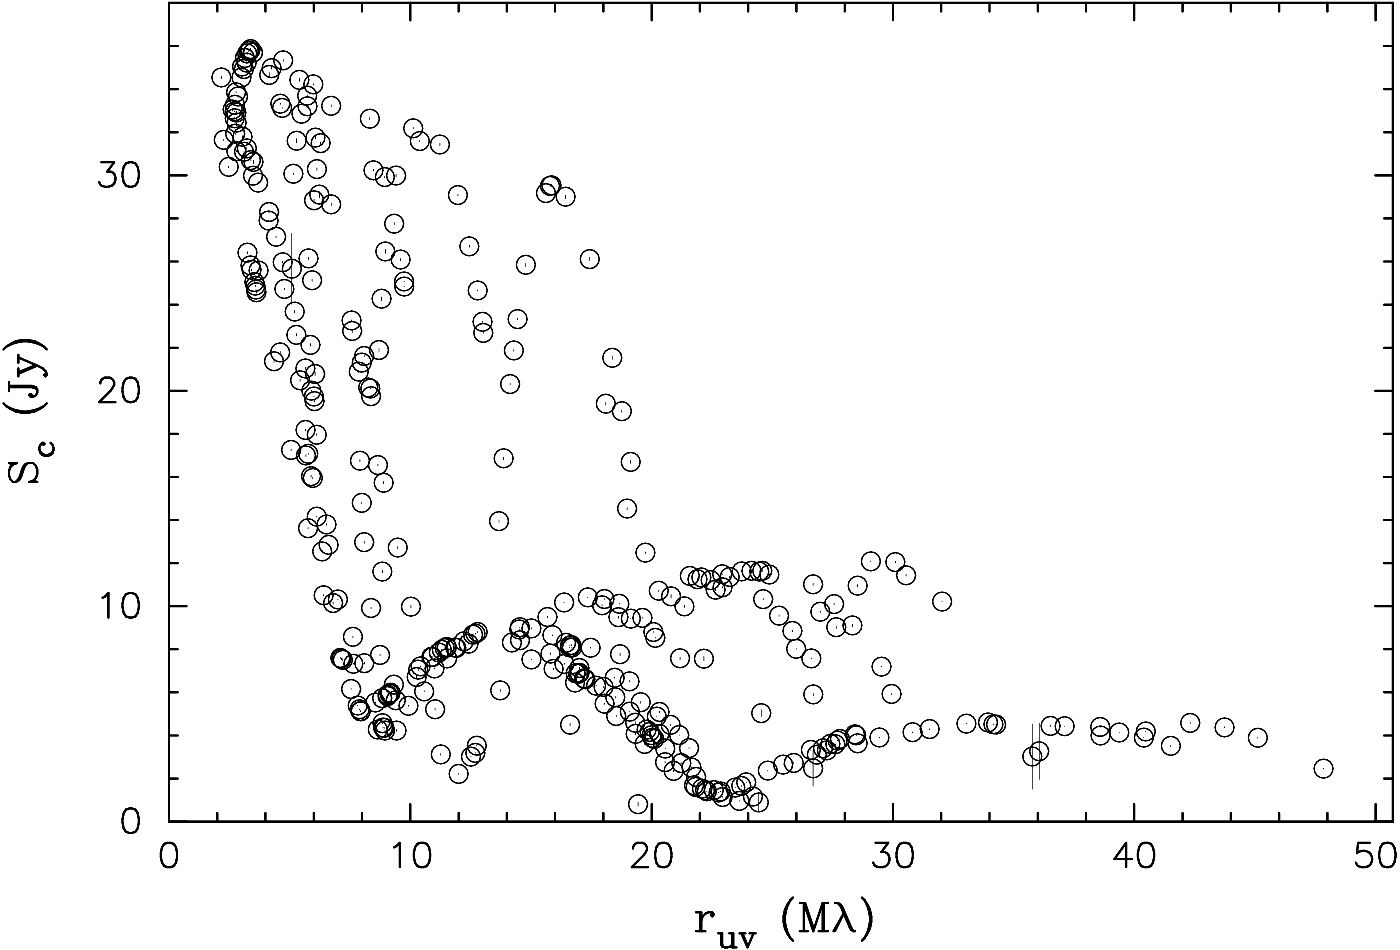
\includegraphics[width=0.56\textwidth,trim = -0.1cm 0cm 0cm -1cm]{J1229+02_L_2011_08_18_yyk_rad.pdf}
}
\caption{Результаты наземных РСДБ наблюдений на VLBA квазара 3C\,273 на \SI{15}{\GHz} (вверху, 10
февраля 2013 г., пик интенсивности \SI{3.2}{\jansky\per\beam}, уровень шума
\SI{1.4}{\milli\jansky\per\beam}, размер диаграммы направленности $1.21\times0.53$\,\si{\mas}) и
\SI{1.6}{\GHz} (внизу, 18 августа 2011 г., пик интенсивности \SI{9.6}{\jansky\per\beam}, уровень
шума \SI{2.2}{\milli\jansky\per\beam}, размер диаграммы направленности $10.6\times4.4$\,\si{\mas}).
Слева: изображение полной интенсивности в условных цветах и контурах, диаграмма направленности на
уровне половины мощности обозначена зелёным эллипсом. Контуры начинаются с 0.25\,\% и 0.07\,\% от
пика интенсивности и идут с шагом $\times2$ на \SI{15}{\GHz} и \SI{1.6}{\GHz} соответственно.
Желтые линии на изображении 15~ГГц показывают диапазон позиционных углов наземно-космических баз
РадиоАстрона, охватываемых нашими наблюдениями: \ang{10}, \ang{-8}, \ang{-38}.
Справа: соответствующая интерферометрическая амплитуда (функция видности) в зависимости от проекции
базы.}
\label{fig:3c273_ground}
\end{figure*}

Квазар 3C\,273 имеет красное смещение $z = 0.158$, находится на расстоянии светимости
\SI{750}{\mega\parsec} и регулярно картографируется в течение последних четырех десятилетий,
включая наблюдения на частоте 15 ГГц на VLBA как часть обзора MOJAVE \cite{Lister_2013}. Как видно
на рисунке~\ref{fig:3c273_ground}, струя быстро становится хорошо разрешенной. Тем не менее,
амплитуда функции видности остается на уровне нескольких Янских до максимальных наземных баз. Это
соответствует яркой детали в видимом основании струи, где оптическая толща приближается к единице.
Предыдущие оценки яркостной температуры для ядра 3C\,273 включают \SI{5e11}{\kelvin} из космических
\cite{Dodson_2008} и до \SI{6e12}{\kelvin} из наземных \cite{Kovalev_2005} РСДБ экспериментов.

Здесь мы сообщаем результаты космических РСДБ наблюдений 3C\,273 на длинах волн 1.3, 6.2 и 18 см на
базах интерферометра между КРТ и 100 м телескопом NRAO в Грин-Бэнк (GBT),
фазированным VLA, 100-метровый радиотелескоп в Эффельсберге и 305-м радиотелескопом в обсерватории
Аресибо в период с декабря 2012 по февраль 2013 года. Проекции баз интерферометра доходили до
171\,000\,км и \num{7.6e9}$\lambda$ (подробности см. в таблице~\ref{tab:3c273_results}). Мы
отмечаем, что более поздние наблюдения РадиоАстрона 3C\,273 на 18, 6.2 и 1.3 см вплоть до середины
2015 года не дали никаких детектирований на проекциях баз больше 1.1\,G$\lambda$. Мы принимаем
космологию с $\Omega_m=0.27$, $\Omega_\Lambda = 0.73$ и $H_0 =
\SI{71}{\km\per\second\per\mega\parsec}$ \cite{Komatsu_2009}.

\subsection{РСДБ на РадиоАстроне: наблюдения, корреляция и поиск сигнала}

Наблюдения проводились либо в двух ПЧ каналах шириной \SI{16}{\MHz} для ортогональных круговых
поляризаций в данной полосе частот, либо одновременно в двух полосах частот с одной поляризацией в
каждой полосе. Центральные частоты наблюдений были следующими: \SI{1668.0}{\MHz} (L-диапазон),
\SI{4836.0}{\MHz} (C-диапазон) и \SI{22236.0}{\MHz} (K-диапазон). Для КРТ, после преобразования в
основную полосу, четыре полосы ПЧ 16 МГц были оцифрованы с частотой Найквиста с дискретизацией 1
бит. Оцифровщики и локальные генераторы контролировались высокостабильными водородными часами,
расположенными на каждой антенне, включая КРТ. Поток данных со скоростью
\SI{128}{\mega\bit\per\second} передавался на Землю по нисходящей линии связи \SI{15}{\GHz} на
антенну \SI{22}{\meter}, расположенную в Пущинской радиоастрономической обсерватории под Москвой.
После декодирования данные сохранялись и затем отправлялись по сетевому каналу в Астрокосмический
центр (АКЦ) в Москве, где они коррелировались с данными, записанными с помощью двухбитной выборки в
Аресибо, Эффельсберге, GBT или VLA с использованием  программных корреляторов, разработанных в АКЦ
\cite{Kardashev_2013_rus} и DiFX \cite{Deller_2011,Bruni_2014}.


\begin{table}[]
\caption{Результаты наземно-космических измерений квазара 3C\,273 на РадиоАстроне}
\label{tab:3c273_results}
\centering
\scriptsize
\begin{SingleSpace}
\begin{tabular}{cclcrrrcrccc}
\toprule
$\lambda$ &
Epoch &
GRT &
$r_{uv}$ &
P.A. &
S/N &
$S_\text{t}$ & $S_\text{c}$ & \multicolumn{1}{c}{$\theta$} &
$T_\text{b}$ & $T_\text{b,min}$ & $T_\text{b,char}$ \\
(см) & & & (\SI{e3}{\km}; \si{\giga\la}) & (\si{\degree}) & & (\si{\jansky}) & (\si{\milli\jansky})
& (\si{\uas}) & (\SI{e12}{\kelvin}) & (\SI{e12}{\kelvin}) & (\SI{e12}{\kelvin}) \\
\multicolumn{1}{c}{(1)} &
\multicolumn{1}{c}{(2)} &
\multicolumn{1}{c}{(3)} &
\multicolumn{1}{c}{(4)} &
\multicolumn{1}{c}{(5)} &
\multicolumn{1}{c}{(6)} &
\multicolumn{1}{c}{(7)} &
\multicolumn{1}{c}{(8)} &
\multicolumn{1}{c}{(9)} &
\multicolumn{1}{c}{(10)} &
\multicolumn{1}{c}{(11)} &
\multicolumn{1}{c}{(12)} \\
\midrule
1.3  & 2013-02-02 & Gb, Y27 & 103; 7.6~ &  $-7$ &  9.8 & 3.4 & $125\pm22$ &  26 &  14 & 5.3 & 12 \\
6.2  & 2012-12-30 & Ar, Ef  &  90; 1.45 &   10  & 18.6 & 4.3 & $125\pm17$ & 142 &  13 & 4.5 & 18 \\
6.2  & 2013-02-02 & Ar      & 103; 1.69 &  $-8$ & 11.6 & 4.3 & $123\pm19$ & 122 &  17 & 5.2 & 15 \\
18   & 2013-01-08 & Gb      & 157; 0.87 & $-32$ &  8.9 & 5.0 & $ 42\pm7$  & 275 &  34 & 4.0 & 10 \\
18   & 2013-01-25 & Ar, Gb  & 171; 0.95 & $-38$ & 12.0 & 5.0 & $ 52\pm9$  & 246 &  42 & 6.3 & 18 \\
\bottomrule
\end{tabular}
\end{SingleSpace}

\textbf{Примечания.}
(1) Длина волны наблюдения; (2) дата наблюдения в формате год-месяц-день; (3) наземный
радиотелескоп с которым были получены значимые лепестки (Ef: Эффельсберг; Y27: фазированная VLA;
Ar: Аресибо); (4) средняя проекция базы в линейных размерах и в длинах волн; (5) позиционный угол
базы; (6) максимальное значения соотношения сигнал/шум лепестка на времени интегрирования 9.5
минут; (7) оценка плотности потока ядра (см. подробности в тексте); (8) максимальная измеренная
амплитуда с среднеквадратической ошибкой данного наблюдения, оценка ошибки включает
неопределённость амплитудной калибровки, следуя \cite{Kovalev_2014_rus}; (9) оценка углового
размера наблюдаемой детали, полная ширина на половине максимума круглого Гауссова распределения
яркости; (10) яркостная температура в системе отсчёта источника, соответствующая размеру в колонке
(8); (11 и 12) минимальная и характерная яркостная температура в системе отсчёта источника,
полученная с помощью подхода, предложенного в \cite{Lobanov_2015a}
\end{table}

\begin{figure}[]
\centerfloat{
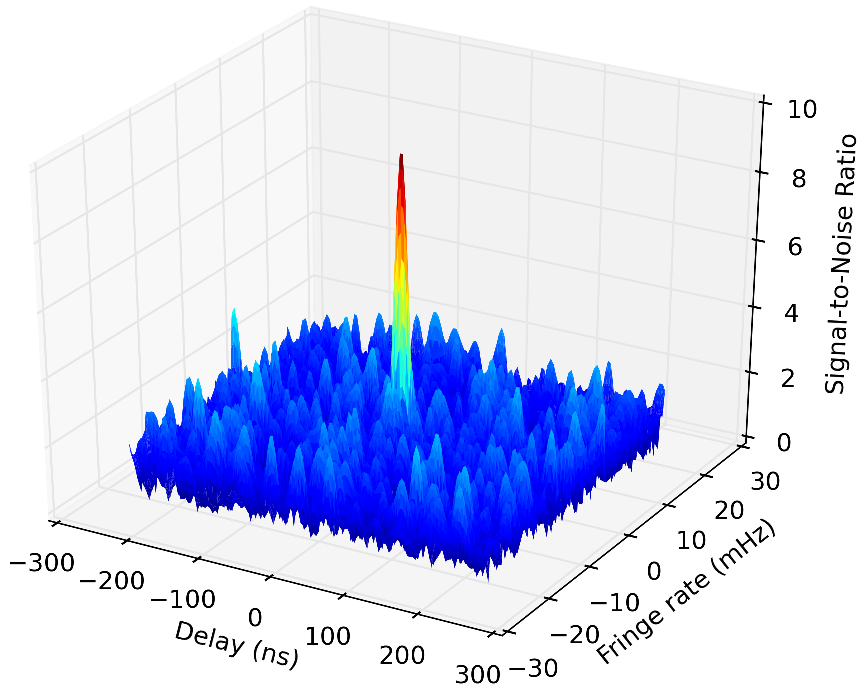
\includegraphics[width=0.47\textwidth,trim = 0cm 0cm 0cm
0cm,clip]{3C273_raes11a_K_GBT-SRT_fringe3D.pdf}
}
\caption{Отклик интерферометра РадиоАстрон (Космический радиотелескоп -- GBT) на \SI{22}{\GHz} при
наблюдении квазара 3C\,273 2 февраля 2013~г. с проекцией базы \SI{7.6}{\giga\la}. Отношение
амплитуды лепестка интерферометра к средней амплитуде шума показано как функция остаточной задержки
(в наносекундах) и частоты интерференции (в миллигерцах).
}
\label{fig:3c273_k_fringe}
\end{figure}

В системе космической РСДБ, где точность определения орбиты ограничена, а неопределенность вектора
базы и его производных по времени велика, необходимо искать интерферометрический отклик в широком
диапазоне пробных задержек, частот задержки и ускорений задержки. Посткорреляционный анализ данных
проводился с использованием программного пакета PIMA \cite{Petrov_2011}, включая подгонку лепестков
с компенсацией за все три параметра. На рисунке~\ref{fig:3c273_k_fringe} показан график амплитуды
лепестка в зависимости от фазовой задержки и частоты интерференции для наблюдений КРТ--GBT 3C\,273
на частоте \SI{22}{\GHz} 2 февраля 2013 года. После применения начальной остаточной задержки
\SI{17.7}{\micro\second}, поправки частоты интерференции \SI{2.45}{\hertz} и остаточное ускорение
менее \SI{3e-16}{\second\per\second^2}, данные были повторно прокоррелированы, так что
интерферометрический отклик кажется около начала координат на рисунке~\ref{fig:3c273_k_fringe}.

Отклик интерферометра, показанный на рисунке~\ref{fig:3c273_k_fringe}, а также значения соотношения
сигнал/шум (S/N), представленные в таблице~\ref{tab:3c273_results}, были интегрированы в течение 9.5
минут. Вероятность ложного детектирования для каждого показанного измерения оценивается как менее
\num{e-12}. Обширные проверки показали, что ни одна из основанных на мазере систем локальных
генераторов, ни на земле, ни на космическом аппарате, не ограничивает когерентность в течение
9.5-минутных интервалов. Интерферометры с базами земля-земля имеют потери когерентности, связанные
со случайными изменениями фазы на пути через атмосферу к обеим станциям. Интерферометры космос-земля
имеют потери когерентности, связанные с распространением через атмосферу только на одну станцию,
поэтому результирующее время когерентности на базах с КРТ длиннее, чем обычно достигается с
системами земля-земля. Наш анализ многих наблюдений РадиоАстрона показал, что после применения
остаточного члена ускорения орбиты к данным в большинстве экспериментов не наблюдается значительных
потерь когерентности в пределах 9.5-минутного интегрирования на 6 и 18 см. Частичная потеря
когерентности происходит при 1.3 см; он влияет на амплитуды лепестков и, следовательно, на отношение
сигнал/шум, измеренное с помощью базовой подгонки лепестков (таблица~\ref{tab:3c273_results},
столбец 6). Остаточные наземные фазовые вариации рискованно компенсировать в случае вырожденных
треугольников земля-космос с низкими S/N на космических базах из-за возможного завышения амплитуды
лепестков (подробности см. \cite{Marti_Vidal_2008}). Из-за этого мы использовали интегрирование 200
с для оценки коррелированных плотностей потоков, показанных в столбце (8)
таблицы~\ref{tab:3c273_results}, поскольку когерентный анализ наземных данных не показал
значительных потерь за этот интервал времени.

\subsection{Яркостная температура}

\subsubsection{Оценка яркостной температуры из модели одиночной Гауссовой компоненты}

Данные наблюдений и оценки основных параметров приведены в таблице~\ref{tab:3c273_results}. Как
наблюдения MOJAVE в феврале 2013 года на частоте 15 ГГц (рисунок~\ref{fig:3c273_ground}, принимая
плотность потока в ядре и предполагая, что его радиоспектр является плоским), так и наши результаты
VLA--GBT на 22 ГГц дают оценку полной плотности потока (на <<нулевой базе>>) компактного ядра как
$S_\text{t} = \SI{3.4}{\jansky}$. Плотность потока ядра на 18 см $S_\text{t} = \SI{5.0}{\jansky}$
оценивается путем моделирования данных VLBA на 18 см (рис.~\ref{fig:3c273_ground}) в предположении,
что его плотность потока существенно не изменилась за 1.5 года после наблюдений VLBA. Это
подтверждается сравнением видностей с нашими измерениями в экспериментах РадиоАстрона на аналогичных
наземных базах. Плотность потока ядра 6.2 см $S_\text{t} = \SI{4.3}{\jansky}$ оценивается путем
интерполяции значений на 18 и 1.3 см со спектральным индексом $\alpha \approx -0.15$ ($S \propto
\nu^\alpha$).

На 1.3 см у нас есть два измерения интерферометра земля-космос, оба на проекциях баз около
\SI{8}{\giga\la}, что соответствует формальному разрешению интерферометра \SI{27}{\uas}. На базах с
РадиоАстроном были продетектированы лепестки как с GBT, так и с VLA с отношением сигнал/шум около 10
(см. рис.~\ref{fig:3c273_k_fringe}). Измеренные амплитуды лепестков на этих базах близки к
\SI{0.1}{\jansky}. Предполагая круговую гауссову модель, это соответствует размерам детали на
\SI{1.3}{\cm} около \SI{26}{\uas} или 2.7 световых месяцев. Мы подчеркиваем, что оценки размера и
яркостной температуры, представленные в таблице~\ref{tab:3c273_results}, относительно
нечувствительны к неопределенности в плотности потока на нулевой базе и к ошибкам в измеренной
амплитуде лепестков.

Длина наибольшей проекции базы, на которой получены лепестки, составила величину 171\,000\,км, между
КРТ и GBT и Аресибо на 18 см. Способность интерферометра измерять яркостную температуру разрешенного
источника зависит от физической длины базы интерферометра (подробнее см. \cite{Kovalev_2005}), и не
зависит от длины волны. Поэтому наши 18-сантиметровые наблюдения РадиоАстрона исследуют самые
высокие значения температуры яркости. Они показывают амплитуду лепестков около
\SI{50}{\milli\jansky}. Соответствующая яркостная температура составляет \SI{4e13}{\kelvin}.
Измерения на 18 см проводились на базе земля-космос с позиционным углом около \ang{-35}, примерно
ортогональным направлению релятивистской струи. Следовательно, если компактный элемент вытянут вдоль
направления струи, он может иметь более низкую яркостную температуру. Однако наше моделирование
наземных наблюдений VLBA на 18 см (рис.~\ref{fig:3c273_ground}) показывает, что продольная
протяженность самой компактной детали не может превышать \SI{0.7}{\mas}. Соответственно, оценка
яркостной температуры на 18 см может уменьшиться максимум в два раза.

\subsubsection{Оценка пределов яркостной температуры}

Пределы яркостной температуры могут быть оценены непосредственно из измерений амплитуды видности в
предположении моделей распределения яркости излучающей области \cite{Lobanov_2015a}. Если
распределение яркости можно описать двумерной гауссовой моделью, то наблюдаемая амплитуда видности
$V\text{r}$, измеренная в области Фурье, $r_{uv}$, определяет минимальную яркостную температуру,
$T_\text{b,min}$, поддерживаемую измерением. Если известны как амплитуда видности, так и ее
среднеквадратичная ошибка $\sigma_{V_\text{r}}$, то можно получить характеристическую яркостную
температуру $T_\text{b,char}$, предполагая, что структурные детали разрешены. Это предположение
приводит к требованию плотности потока на нулевой базе $V_0 \geqslant V_\text{r} +
\sigma_{V_\text{r}}$ \cite{Lobanov_2015a}. Применение этого подхода к данным  крупных наземных РСДБ
обзоров продемонстрировало, что интервал ($T_\text{b,min}$; $T_\text{b,char}$) заключает в себе
температуру яркости наиболее компактной структуры в компактных внегалактических радиоисточниках при
условии, что измерения сделано на расстояниях Фурье более \SI{200}{\mega\la}. Это говорит о том, что
метод хорошо подходит для применения к измерениям РадиоАстрона, проводимым на наземно-космических
базах.

В таблице~\ref{tab:3c273_results} перечислены соответствующие минимальные и характерные яркостные
температуры 3C\,273 в столбцах (11) и (12), полученные из амплитуд видности, измеренных на базах
между наземными антеннами и КРТ. Эти значения могут отличаться от оценок в столбце (10), для которых
были сделаны явные предположения о плотности потока на нулевой базе. Для каждой эпохи в таблице
представлены результаты для наиболее чувствительной базы. Данные о видности, использованные для этих
оценок, сначала были когерентно усреднены в двухминутных интервалах, а затем амплитуды, измеренные
по одному скану РадиАстрона, были использованы для оценки $T_\text{b,min}$ и $T_\text{b,char}$. Эти
пределы подразумевают, что яркостная температура излучения, обнаруженного измерениями РадиоАстрона,
не может быть меньше примерно \SI{5e12}{\kelvin}.

\subsubsection{Обсуждение}

Самые высокие температуры яркости, полученные по нашими измерениями на 18 см, мы оцениваем
$T_\text{b} > \SI{4e13}{\kelvin}$. На этой длине волны увеличение размера из-за рассеяния может быть
существенным и оценки, которые учитывают рассеяние, могут быть ещё выше. Однако недавнее открытие
рефракционной субструктуры в Sgr\,A* \cite{Gwinn_2014} позволяет предположить, что рассеяние в
турбулентной межзвездной среде может привести к переоценке коррелированной плотности потока на
длинных наземно-космических базах с соответствующей переоценкой видимой яркостной температурой
\cite{Johnson_2015} на 18 см. Даже если этот эффект присутствует в наших данных, мы подчеркиваем,
что значения до \SI{2e13}{\kelvin} обнаруживаются на более коротких длинах волн, где рассеяние
слабое, а влияние субструктуры незначительно. Подробный анализ этого эффекта представлен в
сопутствующей статье \cite{Johnson_2016}, которые оценивают, что $T_\text{b} = \SI{7e12}{\kelvin}$
на 18 см. Таким образом, предполагаемые значения яркости, вероятно, будут близки к \SI{e13}{\kelvin}
на каждой длине волны наблюдения.

Видимую экстремальную яркостную температуру в 3С\,273, о которой здесь сообщается, трудно объяснить.
Мониторинг VLBA 3C\,273 на частоте 15 ГГц показывает максимальную наблюдаемую скорость струи
$\beta_\text{app} \approx 15c$ \cite{Lister_2013}, что подразумевает усиление $\delta \lesssim 13$,
согласно оценке \cite{Jorstad_2005} и \cite{Savolainen_2010}. Учитывая комптоновский предел в
\SI{e11.5}{\kelvin} или значение яркостное температуры при равнораспределении \SI{5e10}{\kelvin},
это усиление по меньшей мере в 10--60 меньше, чем требуется, чтобы получить наблюдаемую яркостную
температуру на 18 см, и в 3--20 меньше, чтобы объяснить результаты 1.3 см. Это говорит о том, что
радиоизлучение от 3C\,273 не может быть хорошо описано некогерентным синхротронным излучением от
релятивистских электронов \cite{Kardashev_2000}.

Мы рассмотрели возможность того, что скорости струи, наблюдаемые с помощью VLBA \cite{Lister_2013},
намного ниже, чем объемная скорость потока, относящаяся к доплеровскому ускорению. Тем не менее,
наблюдаемая взаимосвязь между видимой яркостной температурой и видимой скоростью квазаров
соответствует ожидаемой, если скорость потока и скорость рисунка связаны
\cite{Kovalev_2005,Homan_2006}. Другая возможность заключается в том, что инжекция или ускорение
релятивистских электронов достаточны для компенсации потерь из-за обратного комптоновского
охлаждения. Однако для этого необходимо, чтобы ускорение происходило в области, которая должна
находиться в нескольких парсеках от центрального ядра из-за синхротронного самопоглощения ближе к
центральной машине \cite{Blandford_Konigl_1979,Pushkarev_2012}. Более того, \cite{Readhead_1994}
отметил, что устойчивая яркость $\gamma$-излучения, вероятно, потребуется на уровне, который не
наблюдается (см. низкий уровень потока $\gamma$-лучей около эпохи 2013.0 в
\cite{Ramakrishnan_2015}). Количественные расчеты сильно зависят от модели. В
\cite{Petropoulou_2015} определили наблюдательные проявления комптоновской катастрофы и отметили,
что они не были реализованы в 3C\,273. В качестве альтернативы, часть или всё наблюдаемое
радиоизлучение от 3C\,273 может быть связано с синхротронным излучением от релятивистских протонов,
а не электронов, что могло бы увеличить теоретический предел яркостной температуры в
$(m_\text{p}/m_\text{e})^{9/7} \approx \num{1.5e4}$ \cite{Jukes_1967}. Однако это увеличило бы
требуемое магнитное поле в $(m_\text{p}/m_\text{e})^{2} \approx \num{4e6}$, что делает модель
протонного синхротрона проблематичной. Кроме того, в \cite{Rees_1968} указано, что, если частота
наблюдения не ниже гирочастоты электрона, поглощение электронами все еще ограничит наблюдаемые
яркостные температуры каноническими значениями. Это подразумевало бы значения магнитного поля
порядка \SI{e3}{\gauss}, что намного превышает то, что, как считается, существует в струях квазаров.
Модели, учитывающие синхротронное излучение электронно-позитронных потоков с доминированием частиц с
моноэнергетическим распределением частиц \cite{Tsang_2007}, могут согласовываться яркостными
температурами \SIrange[fixed-exponent=14,scientific-notation=fixed]{0.5e14}{2e14}{\kelvin} для
физических условий, измеренных в струе 3C\,273 \cite{Savolainen_2010}, но из-за потерь
синхротронного излучения первоначально монохроматический спектр будет расширен. Когерентные или
коллективные процессы, такие как плазменные волны или стимулированное синхротронное излучение
\cite{Melrose_1999} или циклотронное излучение \cite{Begelman_2005}, также могут привести к
яркостным температурам, значительно превышающим \SI{e12}{\kelvin}.

Поскольку наши наблюдения обнаруживают эти экстремальные значения яркости в широком диапазоне
частот только в течение периода около двух месяцев~"--- меньше, чем время пересечения света,"---
они также могут указывать на существование кратковременного явления, которое уводит излучающую
плазму от равнораспределения. Тем не менее, идентификация такой переменной области с ядром струи
может быть сложной задачей из-за синхротронной непрозрачности и ожидаемых временных задержек между
частотами. Тем не менее, местоположение ядра все еще более вероятно для этого излучения, поскольку
оптически тонкая струя 3C\,273 не показала очень ярких неразрешенных узлов ни в каких наблюдениях,
полученных из предыдущих наземных программ мониторинга. Мы отмечаем, что временная шкала
обратных комптоновских потерь должна составлять около одного дня или меньше на этих частотах,
согласно оценкам \cite{Slysh_1992,Readhead_1994}.

\subsection{Заключение}

Многочастотные наблюдения на частотой 1.7, 4.8 и 22 ГГц, выполненные с помощью РСДБ миссии
РадиоАстрон, выявили чрезвычайно компактную структуру в струе архетипического квазара 3C\,273 с
интерферометрическими детектированиями до 13.5 диаметров Земли, которая вероятнее всего является
его видимым ядром. По оценкам, яркостная температура ядра достигает значений, превышающих
\SI{e13}{\kelvin}. Субструктура, вносимая межзвездным рассеянием \cite{Johnson_2016}, может
существенно повлиять на оценки на 1.7 ГГц. В то же время наши значения яркостной температуры в
диапазоне 4.8 или 22 ГГц остаются неизменными. Мы заключаем, что трудно интерпретировать данные в
терминах обычного некогерентного синхротронного излучения. Текущий анализ большой выборки AGN на
длинных базах РадиоАстрона поможет раскрыть эту загадку.


\section{PKS 1954\textminus388: RadioAstron Detection on 80,000 km Baselines and
Multiwavelength Observations}

\subsection{Введение}

Основной проблемой в астрономии является борьба за наблюдение объектов с угловым разрешением,
достаточным для исследования основных физических механизмов. Более длинные волны радиоастрономии
изначально затрудняли поиск высокого углового разрешения, но относительная простота сохранения
фазовой информации позволила использовать метод интерферометрии со сверхдлинными базами (РСДБ).
Межконтинентальная РСДБ на регулярной основе достигает угловых разрешений на уровне миллисекунд
дуги, а расширение баз между телескопами в космос с помощью спутниковых телескопов, в настоящее
время даёт самое высокое угловое разрешение, достигаемое в астрономии.

В этой статье мы описываем многочастотные исследования PKS 1954-388 на решетке Compact Array в
Австралии (ATCA, максимальная база 6~км) и представляем РСДБ изображение, полученное на
8.4~ГГц на  TANAMI (максимальная база $\sim$10\,000~км) и наблюдение в рамках обзора активных ядер
галактик (АЯГ) на РадиоАстроне на частоте 1.66~ГГц (максимальная база $\sim$80\,000~км или 6.2
диаметра Земли). Рассматривается выраженная переменность источника в радио и гамма-излучении, и мы
объединяем их с данными спутников Swift и Fermi для получения спектрального распределения энергии
(SED) для источника, который соответствует самосогласованной модели.

\subsection{PKS 1954\textminus388}

PKS\,1954\textminus388 был впервые каталогизирован в обзоре Паркса на частоте 2.7~ГГц
\cite{Shimmins_1971}. Источник наблюдался в мае 1969 года с плотностью потока
\SI{2.00+-0.05}{\jansky} и снова в июне 1970 года с плотностью потока \SI{1.50+-0.05}{\jansky} и был
отмечен как возможно переменный. Сравнение с каталогом Molonglo 408 МГц показало инвертированный
спектр, что вызвало последующие оптические наблюдения на 74-дюймовом (1.9 м) телескопе Mt Stromlo,
что позволило идентифицировать галактику 18-й величины \cite{Shimmins_1971a}. Ранние наблюдения с
помощью 3.9~м англо-австралийского телескопа дали красное смещение $z = 0.63$ \cite{Browne_1975}.

Открытие высокого уровня оптической поляризации, 11\,\% \cite{Impey_1988}, привело к
классификации источника как блазара. \cite{Oshlack_2002} использовали измерения ширины
линии $\text{H}\beta$ и светимости, чтобы оценить массу центральной черной дыры
\num{4.3e8}\,$\text{M}_\odot$ для источника.

PKS\,1954\textminus388 не был обнаружен прибором EGRET в Комптоновской гамма-обсерватории. Однако
свойства радио привели Vercellone et al. (2004), чтобы классифицировать источник в качестве
потенциального гамма-излучения AGN, предсказание подтверждается обнаружением источника с помощью
\emph{Fermi} Large Area Telescope \cite{Abdo_2010}. Исследования \cite{Nolan_2012} указывают,
что источник является переменным на энергиях гамма-излучения, с вероятностью <1\,\%, что поток
будет устойчивым, поведение, характерное для класса AGN.

Этот источник был включен в обзор AGN на VSOP \cite{Hirabayashi_2000}, хотя он не наблюдался до
окончания миссии. Однако включение в список обследований привело к тому, что в период с октября 1996
года по февраль 1996 года источник стал частью программы мониторинга нескольких эпох с ATCA на
частотах 1.4, 2.5, 4.8 и 8.6~ГГц. Это выявило выраженную переменность на более высоких частотах, но
нет никаких доказательств на частоте 1.4 ГГц для какой-либо переменности на масштабах времени
$\sim$70 дней \cite{Tingay_2003}.

Серия РСДБ наблюдений~"--- на частоте 4.9~ГГц в мае 1993 года \cite{Shen_1998}, на частоте
4.9~ГГц в июне 1996 года \cite{Fomalont_2000}, на частоте 15 ГГц в июне 1998 года
\cite{Kovalev_2005} и на 2.3 и 8.6~ГГц в декабре 2002 г. \cite{Pushkarev_Kovalev_2012} --- показали,
что источник с сильным доминированием ядра \cite{Pushkarev_Kovalev_2015}. В более глубоких РСДБ
наблюдениях на частоте 8.4 ГГц в июле 2002 года, помимо ядра, был обнаружен с невысоким уровнем
значимости второй компонент в $\sim$\SI{2.8}{\mas} к западу \cite{Ojha_2004}.

В \cite{Piner_2012} использовались 36 эпох РСДБ наблюдений обзора RDV на частоте 8~ГГц
в период между 1994 и 2003 годами для измерения видимых скоростей двух компонентов струи. Оба
компонента демонстрировали движения $\sim$\SI{0.1}{\mas\per\year} с соответствующими кажущимися
скоростями $\num{3.7+-1.8} c$ и $\num{3.7+-1.0} c$ для более слабого внешнего и более яркого
внутреннего компонента, соответственно. Внешний компонент в \cite{Piner_2012} согласуется со
слабым вторичным компонентом в статье \cite{Ojha_2004}.

PKS\,1954\textminus388 является частью многоэпоховой программы TANAMI, и изображение первой эпохи на
частоте 8.4~ГГц от февраля 2008 года представлено \cite{Ojha_2010}. Джет простирается на
$\sim$\SI{5}{\mas} на запад, а для ядра была получена яркостная температура в системе отсчёта
источника \SI{1.5e12}{\kelvin}. В \cite{Bock_2016} сообщалась яркостная темпертура
\SI{2.2e11}{\kelvin} для последующего наблюдения TANAMI в ноябре 2008 года, что указывает на
значительную переменность. Яркостная температура~"--- это поверхностная яркость радиоисточника,
выраженная для удобства через эквивалентную температуру черного тела. Это важный параметр, поскольку
существуют ограничения на внутреннюю яркостную температуру, налагаемые как аргументами обратного
комптоновского охлаждения, так и аргументами равнораспределения (см., например,
\cite{Kellermann_2002} для обзора). Поскольку максимальная измеряемая яркостная температура зависит
от длины базы, лучший способ ограничения измерений~"--- это увеличение баз интерферометра за пределы
поверхности Земли с помощью элемента в космосе. Миссия РадиоАстрон достигла этого с запуском
спутника <<Спектр-Р>> 18 июля 2011 года, когда регулярно проводились наблюдения на частотах 0.3,
1.6, 4.8 и 22~ГГц \cite{Kardashev_2013_rus}.

\subsection{Наблюдения}

\subsubsection{РадиоАстрон}

Наблюдения источника PKS 1954-388 в рамках обзора AGN в проекте РадиоАстрон были выполнены на
частоте 1.66 ГГц 23 августа 2012 года с кодом наблюдения raes03br. Наблюдение в режиме моментального
снимка началось в 15:45 UT и продолжалось 1 час с использованием спутника <<Спектр-Р>> и телескопов
Parkes 64~м и Mopra 22~м. На частоте 1.66~ГГц спутник формирует данные в правой круговой поляризации
с шириной полосы 16~МГц с дискретизацией в 1~бит. Бит четности добавляется для каждого байта и
данных, передаваемых на Землю со скоростью \SI{144}{\mega\bit\per\second}. Наземные телескопы
записывают данные в двух полосах ПЧ шириной 16~МГц в двух поляризациях, с 2-битной дискретизацией
данных, обеспечивающей скорость передачи данных \SI{256}{\mega\bit\per\second}.

\begin{figure}[]
\centerfloat{
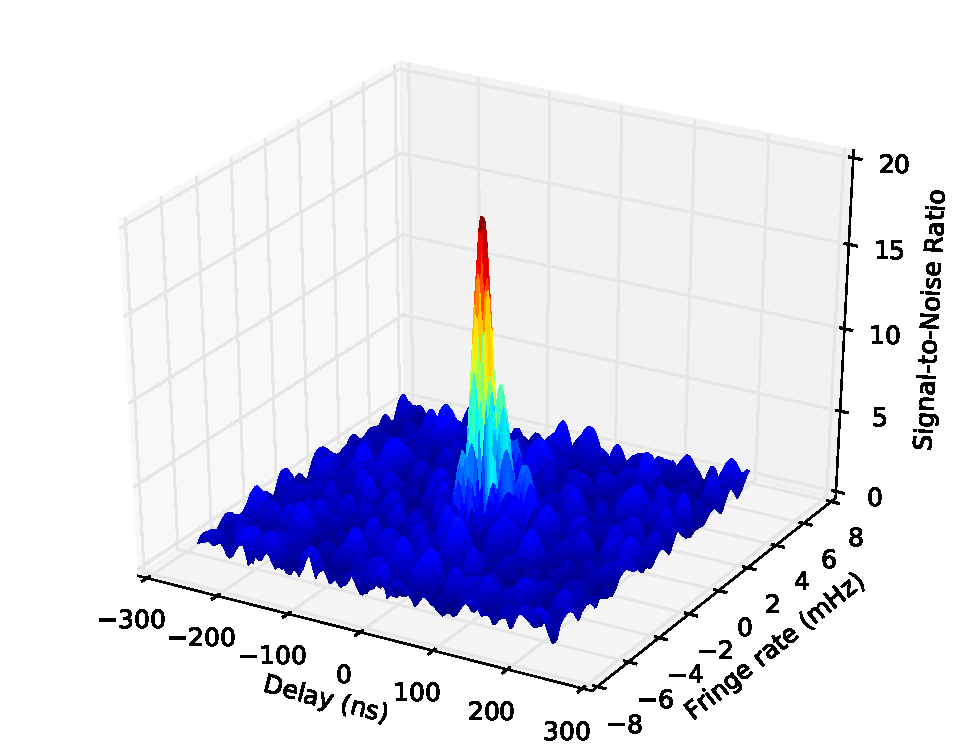
\includegraphics[width=0.7\textwidth,trim = 0cm 0cm 0cm
0cm,clip]{1954-388_raes03br_L_RA-PA_fringe3D.pdf}
}
\caption{Продетектированный лепесток на 1.66~ГГц в пространстве (задержка, частота интерференции)
от PKS\,1954\textminus388 между 64-м телескопом Паркс и спутником РадиоАстрон (Спектр-Р).}
\label{fig:pks_1954_fringe}
\end{figure}

Данные с космического аппарата передавались в режиме реального времени на станцию слежения в
Пущино и записывались на диск. Данные с наземных радиотелескопов записывались на диск, а затем
преобразовывались в формат Mark~5B и передавались в электронном виде в Астрокосмический
центр (АКЦ). Данные были прокоррелированны на корреляторе ASC \cite{Kardashev_2013_rus}, с явными
лепестками на частоте 1.6 ГГц между тремя телескопами (см. рисунок~\ref{fig:pks_1954_fringe}).
Данные были экспортированы из коррелятора и приведена подгонка лепестков в программном пакете PIMA
\cite{Petrov_2011}. $(u, v)$-покрытие для наблюдения, как и ожидалось для режима моментального
снимка, очень скудное, с проекцией базы Паркс-Мопра, равной $\sim$\SI{1}{\mega\la}, и базами для
космического аппарата в диапазоне от 403 до \SI{440}{\mega\la}, 5.8 до 6.2 диаметров Земли, с
позиционным углом $\sim$\ang{177}. Цель обзора AGN~"--- определить, можно ли продетектировать
источники на различных проекциях баз интерферометра, и использовать эту информацию для определения
угловых размеров и соответствующих яркостных температур.

Первоначально амплитуды и отношения сигнал/шум (SNR) были построены как функция времени
интегрирования для каждой базы на каждом скане, чтобы оценить время когерентности. Для этого
наблюдения не оказалось значительных потерь при времени интегрирования до 10 минут. Космические РСДБ
лепестки были обнаружены на 10 минутах интегрирования с SNR = 20 на базах до Паркса и SNR = 7 на
базах до Mopra, что соответствует вероятности ложного детектирования на наземно-космических базах
значительно меньше, чем \num{e-6}.

\begin{figure}[]
\centerfloat{
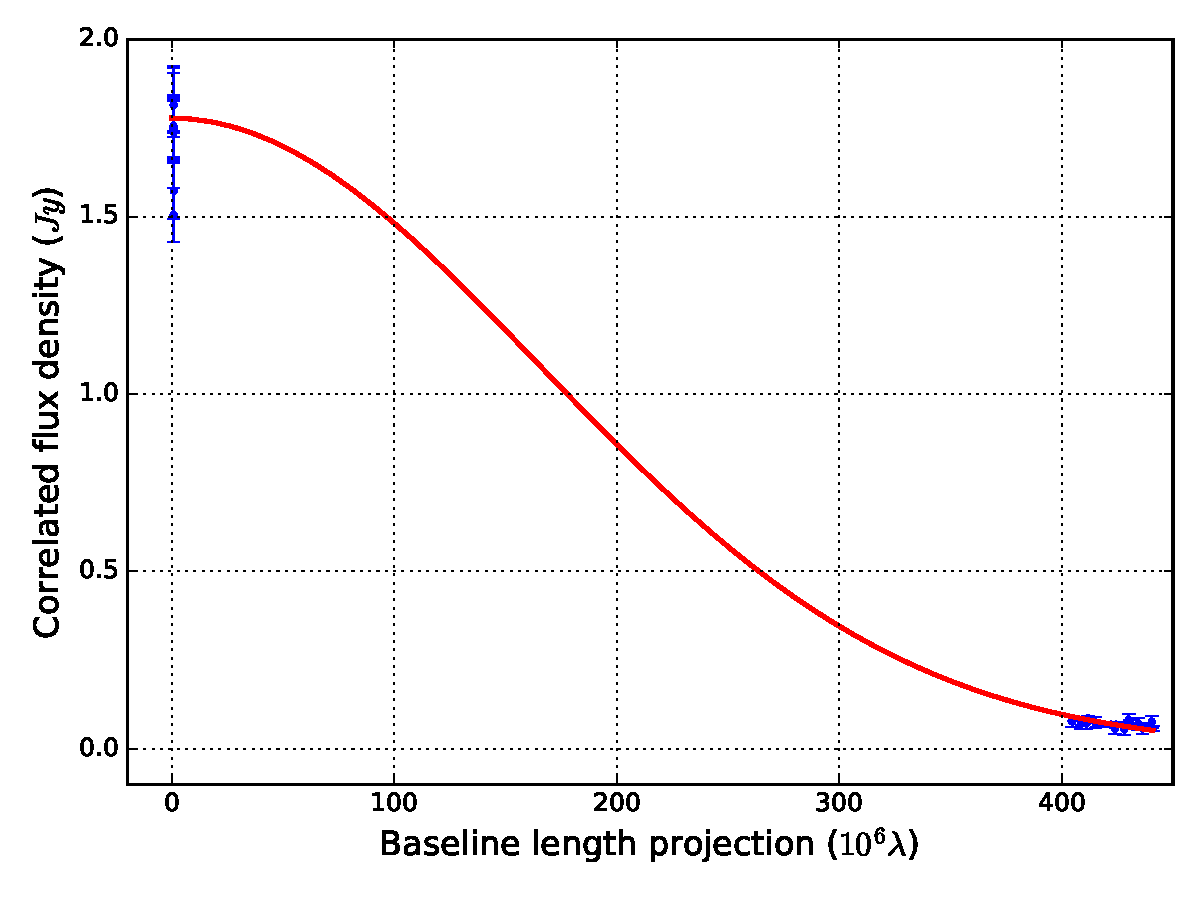
\includegraphics[width=0.7\textwidth,trim = 0cm 0cm 0cm
0cm,clip]{1954-388_raes03br_RADPLOT_w_gaussian.pdf}
}
\caption{График зависимости коррелированной плотности потока от проекции базы для
PKS\,1954\textminus388 на \SI{1.66}{\GHz}. Синие точки~"--- полученные данные: внутренние точки
соответствуют базе Паркс-Мопра, внешние точки~"--- наземно-космические базы с КРТ. Красная
кривая~"--- подгонка простейшей Гауссовой модели (см. подробности в тексте).}
\label{fig:pks_1954_radplot}
\end{figure}

Коррелированная плотность потока \SI{1.78}{\jansky} была измерена на базе Паркс--Мопра, и
$\sim$\SI{0.07}{\jansky} на базе Земля-космос. Самое простое подгонка модели к данным~"---
это один круговой Гауссов компонент с полной плотностью потока \SI{1.78}{\jansky} и шириной на
половине высоты (FWHM) \SI{0.47}{\mas} (см. рисунок~\ref{fig:pks_1954_radplot}). Круглый гауссов
компонент был принят для простоты, хотя размер сильно ограничен в направлении север-юг, но плохо
определен в направлении восток-запад. Вслед за \cite{Kovalev_2005}, мы рассчитываем яркостную
температуру в системе отсчёта наблюдателя \SI{3.6e12}{\kelvin} для этой модели. Ограниченное $(u,
v)$-покрытие означает, что мы не можем быть уверены, что подгонка одной гауссовой модели-компонента
к наземно-наземным и наземно-космическим данным является правильным приближением, и на самом деле
весьма вероятно, что база север-юг (Паркс-Мопра) отражает некоторые структуры в струе к западу от
ядра (см. Разделы 2 и 3.2). Однако существует очень консервативная минимальная яркостная
температура, связанная только с наземно-космическими данными: следуя \cite{Lobanov_2015a}, мы
вычисляем формальную минимальную яркостную температуру в системе отсчёта наблюдателя, равную
\SI{1.3e12}{\kelvin}. Эти значения должны быть умножены на $(1 + z)$ для получения соответствующей
яркостной температуры в системе отсчёта источника. С учетом ожидаемых погрешностей калибровки
простая подгонка, которая эффективно обеспечивает верхний предел, дает яркостную температуру в
системе отсчёта источника \SI{6(1)e12}{\kelvin}, а минимальная яркостная температуру в системе
отсчёта источника составляет \SI{2e12}{\kelvin}, соответственно.

\subsection{Обсуждение}

\subsubsection{Яркостная температура и рассеяние}

Нижний предел температуры яркости исходного кадра, равный \SI{2e12}{\kelvin}, значительно превышает
предел яркостной температуры при равнораспределении, равный $\sim$\SI{5e10}{\kelvin}
\cite{Readhead_1994}, и обратный комптоновский предел, равный $\sim$\SI{e11.5}{\kelvin}
\cite{Kellermann_1969,Readhead_1994}, подразумевая минимальный Доплер-фактор, равный 40 (для
равнораспределения) и 6 (для обратного Комптона). Лоренц-фактор, равный 5, и угол наклона к лучу
зрения \ang{5}, использованный в Модели B подгонки SED (раздел 3.6), подразумевают Доплер-фактор,
равный $\sim$9, и следовательно согласуются с обратным комптоновским Доплер-фактором и с видимой
скоростью $\sim3.7c$ (раздел 2). Доплер-фактор для случая равнораспределения согласовать гораздо
сложнее.

Однако необходимо учитывать влияние рассеяния на источник со стороны межзвёздной среды. Простое
круговое гауссово моделирование радиоастрономических наблюдений PKS\,1954\textminus388,
использованное в разделе 3.1, дает размер ядра \SI{0.47}{\mas}, и если мы предположим, что только
часть плотности потока на базу Паркс--Мопра (но вся на наземно-космической базе) относится к ядру,
то ядро окажется ещё более компактным. Установленный угловой размер замечательно согласуется с
угловым уширением, предсказанным моделью NE2001 для галактической электронной плотности
\cite{Cordes_2002} для <<среднего>> режима видности \cite{Goodman_1989,Taylor_1993} по направлению к
PKS\,1954\textminus388 ($l = \ang{1.6}$, $b = \ang{-29}$). Хотя межзвёздная среда имеет сложную
структуру, и модель NE2001 нельзя использовать для надежного определения рассеивающих свойств вдоль
конкретного направления, результат показывает, что собственный размер ядра на частоте 1.66~ГГц может
быть значительно меньше измеренного, а яркостная температура, соответственно, выше.

Однако, как обсуждалось в \cite{Johnson_2015}, также необходимо учитывать влияние рефракционной
субструктуры, возникающей при рассеянии в межзвёздной среде. Рефракционная субструктура была
обнаружена в некоторых наблюдениях пульсаров РадиоАстрона \cite{Gwinn_2016,Popov_2017} и может также
присутствовать в наблюдениях РадиоАстрона 3C\,273 \cite{Johnson_2016}. Это может иметь эффект
увеличения детектирований на длинных базах РадиоАстрона из-за появления мелкомасштабной структуры в
изображении разрешенного рассеянного источника, что приводит к переоценке внутренней яркостной
температуры.

Мы отмечаем, что \cite{Pushkarev_Kovalev_2015} получают средний размер ядра для
PKS\,1954\textminus388, равный \SI{1.0+-0.2}{\mas} на \SI{2.3}{\GHz} и \SI{0.35+-0.05}{\mas} на
\SI{8.4}{\GHz}, и зависимость частоты от размера $\nu^{\num{-0.94+-0.11}}$, на основе нескольких
эпох одновременных наблюдений на 2.3 и 8.4~ГГц. Их результаты показывают, что собственный размер
источника доминирует над уширением из-за рассеяния на частотах выше 2.3~ГГц. Верхний предел углового
размера \SI{0.47}{\mas}, полученный из наблюдений РадиоАстрона PKS\,1954-388, в три раза меньше
углового размера, ожидаемого на частоте 1.66~ГГц из экстраполяции подгонки
\cite{Pushkarev_Kovalev_2015}. Очевидное расхождение в измерении размера ядра может быть связано с
несколькими факторами: (1) размер компонента ядра может изменяться во времени, поскольку плотность
потока источника сильно меняется и была относительно низкой во время наблюдений РадиоАстрона; (2)
ядро, измеренное в \cite{Pushkarev_Kovalev_2015}, разделяется на несколько компонентов при
субмиллисекундном угловом разрешении, подразумевая, что структура является более сложной, чем
объясняется подгонкой простой модели круглого Гаусса к разреженным данным; или (3) на длинных
наземно-космических базах может преобладать рефракционный шум. Наблюдаемая коррелированная плотность
потока, наблюдаемая на РадиоАстроновских базах, составляет, по меньшей мере, $\sim$4\,\% от
плотности потока компактного компонента, что значительно превышает среднеквадратичное значение
рефракционного шума $\sim$1\,\%, предсказанное \cite{Johnson_2015}. Чтобы различать различные
возможности, необходимы дальнейшие наблюдения РадиоАстрона на промежуточных базах менее 6 диаметров
Земли.

Хотя PKS\,1954\textminus388 довольно компактен, имеет плоский радиоспектр и очень переменный, как
видно на кривых блеска на рисунках 4 и 5, отсутствие какой-либо быстрой высоко-амплитудной
переменности на масштабах часов и дней по результатам мониторинга на ATCA в июне 2014 года (раздел
3.3.1) означает, что нет никаких наблюдательных данных о внутрисуточной переменности (IDV), которая
часто связана с рассеянием на межзвёздной среде. Пока еще невозможно определить, связано ли это с
недостаточно компактной структурой в источнике или с отсутствием близкой области с усиленным
рассеянием на луче зрения, или и с тем и другим.

В любом случае детектирование PKS\,1954\textminus388 на базах $\sim$80\,000\,км на частоте 1.6
ГГц может служить обоснованием решения о размещении спутника на эксцентричной девятидневной орбите
с высотой апогея до 350\,000\,км. Длинные космические базы, предоставленные наблюдениями
РадиоАстрона, позволили измерить значительно более высокие яркостные температуры, например,
превышающие \SI{e13}{\kelvin} для 3C\,273 \cite{Kovalev_2016}, а обзор активных ядер
галактик на РадиоАстроне расширит эти исследования до гораздо большей выборки источников
(Ковалев и др., в процессе подготовки). Высокая чувствительность 18-сантиметрового приемника на
борту космического радиотелескопа РадиоАстрон в сочетании с большими наземными телескопами также
приводит к новому пониманию эффектов межзвездного рассеяния.

\subsection{Заключение}

В наблюдении PKS\,1954\textminus388, проведённом в рамках обзора АЯГ на РадиоАстроне в 2012
году, источник был продетектирован на базе 6.2 диаметра Земли, подтверждая наличие компактного
ядра. Получена яркостная температура в системе отсчёта источника \SI{2e12}{\kelvin}, что
предполагает минимальный Доплер-фактор для обратного комптоновского предела, равный 6.
Простейшая интерпретация данных дает размер ядра \SI{0.47}{\mas} (в одном измерении). Если это
завышенная оценка из-за рассеяния в межзвёздной среде, подразумевается меньший размер ядра и более
высокая яркостная температура. С другой стороны, рефракционная субструктура может иметь эффект
улучшения обнаружения на длинных наземно-космических базах, приводя к переоценке яркостной
температуры. Необходимы дальнейшие наблюдения РадиоАстрона на базах менее 6 диаметров
Земли, чтобы различать различные возможности.

Мониторинг на ATCA показывает, что источник изменился в 5 раз по плотности потока на частоте
8.4~ГГц, а наблюдения Ферми показывают изменения в потоке гамма-излучения не менее чем в 10
раз. Радиовспышка, увеличивавшаяся раньше и быстрее на более высоких частотах, последовала за
продолжительным высоким уровнем гамма-излучения в 2013 году с задержкой между событиями $\sim$9
месяцев, сравнимой с тем, что наблюдалось в других блазарах. Наблюдения РСДБ с несколькими эпохами
обнаруживают постоянные компоненты струи, причем самый внутренний компонент на изображении TANAMI
первой эпохи, вероятно, связан с радиовспышкой 1996 года.

Представленные здесь многоволновые данные были объединены с другими данными для получения SED,
который был подогнан с использованием однозонной синхротронной модели. Несмотря на ковариацию между
параметрами модели и не одновременным характером данных, подгонка модели B дает Доплер-фактор
$\sim$9, что согласуется с нижним пределом обратного комптоновского Доплер-фактора 6,
полученного из наблюдения на РадиоАстроне. Доплер-фактор для случая равнораспределения, равный по
меньшей мере 40, объяснить гораздо сложнее.


\section{The high brightness temperature of B0529+483 revealed by RadioAstron and implications for
interstellar scattering}

\subsection{Введение}

Активные Галактические Ядра (AGN) приводятся в действие аккрецией на сверхмассивные черные дыры.
Связанные с этим физические процессы создают струи релятивистских частиц, которые наблюдаются на
радиоволнах, которые имеют высокие видимые яркостные температуры, $T_\text{b}$. Теория
предсказывает, что яркостная температура ограничена комптоновским охлаждением примерно до
\SI{e11.5}{\kelvin} \cite{Kellermann_1981,Readhead_1994}, умноженное на Доплер-фактор $\delta$.
Обнаружено, что последний имеет типичное значение $\delta \sim 10$ из РСДБ наблюдений
сверхсветовых движений в релятивистских струях \cite{Cohen_2007,Savolainen_2010,Lister_2013}.

Яркостная температуры для источника с круговым гауссовым распределением яркости измеряется как
$T_\text{b} = 2 \ln 2S\lambda^2 (1 + z) / (\pi k_\text{b} \theta^2)$, где $S$~"--- измеренная
плотность потока, $\theta$~"--- угловой диаметр излучающей области (полная ширина на половине
максимума, FWHM), $z$~"--- космологическое красное смещение источника, $\lambda$~"--- длина волны
наблюдения, а $k_\text{b}$~"--- постоянная Больцмана (все значения в единицах СИ). В случае РСДБ
минимальный размер, который может быть измерен, ограничен угловым разрешением до $\theta_\text{lim}
\approx \lambda / B$, где $B$~"--- максимальная проекция базы интерферометра. Размер Земли
ограничивает яркостную температуру, которая может быть измерена наземным РСДБ, до примерно
\SI{e12.5}{\kelvin} для типичной плотности потока \SI{1}{\jansky}. Более высокие значения могут
быть непосредственно получены только с помощью космической РСДБ \cite{Kovalev_2005}, в которой
один из телескопов вращается вокруг Земли, или косвенными измерениями, например, с использованием
межзвездной сцинтилляции (например, \cite{Lovell_2008}).

Миссия космической РСДБ РадиоАстрон сочетает в себе 10-метровый космический радиотелескоп (КРТ) на
борту спутника <<Спектр-Р>>, который находится на высокоэллиптической орбите с апогеем до
370\,000\,км \cite{Kardashev_2013_rus} и наземные радиотелескопы. РадиоАстрон обеспечивает
прямой способ измерения яркостных температур, значительно превышающих \SI{e13}{\kelvin}. Недавно
было показано, что некоторые квазары действительно имеют $T_\text{b} > \SI{e13}{\kelvin}$
\cite{Kovalev_2016,Gomez_2016}. Это создает проблему для современного понимания физики струй. В
частности, для объяснения результатов РадиоАстрона может потребоваться гораздо более высокий
Доплер-фактор, чем это следует из отслеживания сверхсветовых компонентов с помощью РСДБ.

Однако, когда речь идет о наблюдениях с чрезвычайно высоким угловым разрешением с помощью
космического РСДБ, существует другой эффект, который может повлиять на измерения яркостной
температуры. Недавно было показано, что рефракционное рассеяние на межзвездной плазме может
создавать компактные особенности в разрешенных изображениях протяженных радиоисточников, называемых
рефракционной субструктурой \cite{Johnson_2015}. Этот эффект наблюдался в Sgr\,A* на наземных РСДБ
решётках \cite{Gwinn_2014} и в наблюдениях РадиоАстрона квазара 3C\,273 на 18\,см
\cite{Johnson_2016}. Основным эффектом рефракционной субструктуры является появление небольшой
коррелированной плотности потока на длинных базах, даже на базах, где источник был бы полностью
разрешён при отсутствии рассеяния \cite{Johnson_2015}.

Квазар 87GB 0529+483 (J0533+4822, далее B0529+483) занесен в каталог 87GB как имеющий
плотность потока \SI{619+-70}{\milli\jansky} на 4.9~ГГц со спектральным индексом между 80 и 6~см
\num{-0.1} (где $S \propto \nu^\alpha$) \cite{Gregory_Condon_1991,Becker_1991}. Плоский спектр
подразумевает компактную структуру, которая в сочетании с расположением источника на галактической
широте $b = \ang{+8}$ повышает вероятность того, что на источник может повлиять рассеяние. Источник
наблюдался в 29 экспериментах РадиоАстрона, и значимая коррелированная плотность потока была
обнаружена на проекциях базы до 19 диаметров Земли. Эти два факта делают его подходящим
объектом для измерения его яркостной температуры и изучения эффектов рефракционной субструктуры. В
этой статье мы анализируем коррелированные плотности потока (то есть амплитуды видности),
измеренные РадиоАстроном для B0529+483, чтобы получить угловые размеры и яркостные температуры
его наиболее компактных деталей. Кажущаяся яркостная температура оценивается в
системе отсчёта источника с учетом красного смещения $z = 1.162$ \cite{Halpern_2003}, но не
корректируется за доплеровское усиление. Мы обсуждаем два сценария, с и без обнаруживаемой
субструктуры, созданной рефракционным рассеянием в межзвездной среде нашей Галактики.

\subsection{Наблюдения}

\subsubsection{РадиоАстроновские наблюдения}

Наблюдения B0529+483 являются частью обзора AGN ключевой научной программы РадиоАстрон (Ковалев и
др., в процессе подготовки). Список экспериментов, которые содержат этот источник и которые были
выполнены до 1 января 2015 года, показан в таблице~\ref{tab:0529_exper}. Обзор охватывает три
полосы: L со средней частотой \SI{1668}{\MHz} ($\lambda = \SI{18}{\cm}$), C на \SI{4836}{\MHz}
($\lambda = \SI{6}{\cm}$) и K на \SI{22236}{\MHz} ($\lambda = \SI{1.3}{\cm}$). Отметим, что для
наблюдений, полученных до декабря 2012 г., центральные частоты были на \SI{8}{\MHz} ниже для всех
трех полос. Во время обзора AGN RadioAstron использовал режим наблюдения, в котором две полосы
записывались одновременно. Напротив, наземные телескопы обычно наблюдали в одной полосе.
Исключениями были Эффельсберг и Евпатория, которые переключались между диапазонами в течение
наблюдений. Каждый эксперимент обычно длился 40 минут, разделенный на четыре скана по
\SI{600}{\second} каждый. Успешные детектирования интерференционных лепестков  на
наземно-космических базах сгруппированы примерно в 5 месяцев с октября 2012 года по февраль 2013
года.

\begin{table}
\caption{Список РадиоАстроновских экспериментов в которых наблюдался B0529+483. Наземные телескопы,
с которыми был получен значимый сигнал на наземно-космических базах, подчёркнуты. Проекция баз
приведена в диаметрах Земли (E.D.). Сокращения названий телескопов: Bd\,=\,Бадары 32\,m,
Gb\,=\,Green Bank 100\,m, Ef\,=\,Effelsberg 100\,m, Ev\,=\,Евпатория 70\,m, Kl\,=\,Калязин 64\,m,
Mc\,=\,Medicina 32\,m, Nt\,=\,Noto 32\,m, Ro\,=\,Robledo 70\,m, Sv\,=\,Светлое 32\,m, Tr\,=\,Torun
32\,m, Wb = Westerbork Synthesis Radio Telescope, Ys\,=\,Yebes 40\,m, Zc\,=\,Зеленчукская 32\,m.}
\label{tab:0529_exper}
\centering
\small
\begin{SingleSpace}
\begin{tabular}{lllr}
\toprule
Exp.     & Observing   & Frequency, GHz, & E.D. \\
code     & epoch       & and GRTs        & \\
\midrule
raes03dk & 2012 Sep 29 & 4.8: \underline{Wb}, \underline{Ys}; & 7 \\
         &            &  22: Nt, Gb, Ro\\
raes03el & 2012 Oct 25 & 1.7: \underline{Zc}, Ev; 4.8: \underline{Bd} & 3.5 \\
raes03en & 2012 Oct 16 & 1.7: \underline{Zc}, \underline{Ro}; 4.8: \underline{Bd}, \underline{Ev} &
4.5 \\
raes03eo & 2012 Oct 16 & 1.7: \underline{Zc}; 4.8: \underline{Bd}, \underline{Ev} & 5.5 \\
raes03er & 2012 Oct 24 & 1.7: Ro & 3.5 \\
raes03eu & 2012 Oct 24 & 4.8: \underline{Ys} & 2.5 \\
raes03hk & 2012 Dec 09 & 4.8: Ys; 22: Gb, Nt, Ro & 16 \\
raes03hm & 2012 Dec 10 & 4.8: Bd; 22: Gb, Zc & 18 \\
raes03hv & 2012 Dec 15 & 4.8: \underline{Ys}, \underline{Mc}; 22: \underline{Gb} & 5 \\
raes03ia & 2012 Dec 16 & 4.8: \underline{Ef}, Mc; 22: Ef, Ys & 15 \\
raes03kg & 2013 Jan 25 & 1.7: Ev; 4.8: \underline{Ef} & 5 \\
raes03kj & 2013 Jan 26 & 4.8: \underline{Ef} & 11 \\
raes03kk & 2013 Jan 27 & 1.7: \underline{Gb}, Wb; 4.8: Ef & 16 \\
raes03kn & 2013 Jan 28 & 1.7: Wb; 4.8: \underline{Ef}, Mc & 19 \\
raes03kr & 2013 Feb 02 & 1.7: \underline{Wb}, \underline{Mc}; 4.8: \underline{Ys}, Tr & 3 \\
raes03ks & 2013 Feb 02 & 4.8: \underline{Tr}; 22: Ys & 2 \\
raes03kw & 2013 Feb 03 & 1.7: \underline{Tr} & 6 \\
raes03kz & 2013 Feb 03 & 1.7: \underline{Tr}, Ev, Ro & 8 \\
raes03lb & 2013 Feb 04 & 1.7: \underline{Wb}, Bd, Tr; & 12 \\
         &             & 4.8: \underline{Sv}, Zc, Ys &  \\
raks01ct & 2013 Sep 23 & 1.7: Gb, Tr; 4.8: Gb, Ys & 16 \\
raks01cx & 2013 Sep 24 & 1.7: Zc, Bd, Gb, Tr;& 19  \\
         &             & 4.8: Sv, Ef, Ys  & \\
raks01da & 2013 Sep 24 & 1.7: Bd, Tr; 4.8: Sv, Ys & 20  \\
raks01dq & 2013 Oct 01 & 1.7: Bd, Wb, Zc, \underline{Gb}; & 12 \\
         &             & 4.8: \underline{Ef}, Ys, Sv &  \\
raks01ea & 2013 Oct 03 & 1.7: Bd, Gb, Nt, Tr;   \\
         &             & 4.8: Sv, Ev, Ef, Ys & 21 \\
raks01ex & 2013 Oct 11 & 1.7: Zc, Gb, Tr; & 21  \\
         &             & 4.8: Sv, Ev, Wb  & \\
raks08cx & 2014 Oct 15 & 1.7: Kl, Bd, Tr, Ro; & 20  \\
         &             & 4.8: Sv, Zc, Nt  & \\
raks08dc & 2014 Oct 17 & 4.8: Ef, Wb, Ys, Kl, Zc, Tr; & 15  \\
         &             &  22: Gb, Ef, Ys, Tr  & \\
raks08fv & 2014 Nov 13 & 1.7: Kl, Sv, Tr; & 13  \\
         &             & 4.8: Ys, Kl, Bd  & \\
raks08gq & 2014 Nov 20 & 1.7: Gb, Kl, Sv, Zc, Tr; & 17  \\
         &             & 4.8: Ys, Kl, Nt, Tr & \\
\bottomrule
\end{tabular}
\end{SingleSpace}
\end{table}

Корреляция всех этих экспериментов была выполнена на корреляторе АКЦ \cite{Likhachev_2017}.
Эксперименты raes03kg, raes03kj, raes03kk и raes03kn (таблица 1) также скоррелированны с
использованием расширенной версии \cite{Bruni_2016} коррелятора DiFX \cite{Deller_2011}. Наше
сравнение данных двух корреляторов показало, что они дают схожие результаты.

\subsubsection{Измерение амплитуд}

Посткорреляционный анализ данных, включая подгонку лепестков, калибровку полосы пропускания
и амплитуды, а также усреднение было выполнено с использованием пакета PIMA \cite{Petrov_2011}. Это
программное обеспечение имеет несколько важных функций, необходимых для космической РСДБ, описанных
ниже. Кроме того, PIMA оптимизирован для пакетной обработки.

\paragraph{Подгонка лепестков}

Процедура подгонки лепестков в PIMA включает в себя поиск не только остаточной задержки и частоты
интерференции между радиотелескопами, но также и члена ускорения. Этот член важен для
космического РСДБ, поскольку он позволяет нам исправить несовершенные знания об орбите КРТ. Во время
поиска лепестков два частотных канала шириной \SI{16}{\MHz} были объединены для повышения
чувствительности. Для всех успешных детектирований лепестков в экспериментах, которые мы
проанализировали, максимальное отклонение остаточной задержки от ее медианного значения на каждой
базе составило \SI{3.7}{\us}, максимальная частота интерференции соответствует скорости
\SI{3.7}{\cm\per\second}, а максимальное ускорение \SI{5.7e-4}{\cm\per\second^2}.

Статус детектирования для каждого наблюдения определялся вероятностью ложного детектирования (PFD).
Соответствие между отношением сигнал/шум (SNR) и PFD определялось следуя \cite{Petrov_2011}. Короче
говоря, мы подгоняем теоретическое распределение плотности вероятности амплитуды ложных лепестков в
отсутствие сигнала в пространстве параметров <<задержка--частота интерференции--ускорение>> для
полного набора недетектирований в обзоре AGN. Таким образом, мы определяем параметры этого
распределения плотности вероятности для различного числа спектральных каналов, времени
интегрирования и длины скана. Зная эти параметры, мы можем рассчитать PFD для заданного значения SNR
в каждом эксперименте.

Детектирование считается значимым, если SNR соответствует $\text{PFD}<\num{e-4}$. Для одного
эксперимента raes03kn мы нашли значение, превышающее это, но ниже, чем \num{e-3}. Поскольку величина
задержки оказалась меньше \SI{0.5}{\us}, а скорость меньше \SI{0.03}{\cm\per\second}, мы пришли к
выводу, что это также значимое детектирование.

\paragraph{Амплитудная калибровка}

Каждый эксперимент, проанализированный в этой статье, содержит только 2 или 3 базы с очень
разреженным покрытием $(u, v)$-плоскости, поэтому мы не можем применять стандартные методы
калибровки, использующие величины замыкания. Вместо этого была применена априорная калибровка
амплитуды с использованием коэффициентов усиления антенны и измерений температуры системы,
выполненных на каждой антенне во время наблюдения. Для Евпаторийского радиотелескопа эта информация
была недоступна для отдельных экспериментов, поэтому нам пришлось использовать стандартные значения
системной температуры. В двух экспериментах raes03eo и raes03en на частоте \SI{4.8}{\GHz} сигнал
был обнаружен на трех базах, которые образуют почти вырожденный треугольник, что позволяет
нам корректировать усиление Евпатории. Треугольник имеет две базы, которые намного длиннее
третьей. Мы предполагаем, что амплитуды на двух самых длинных базах идентичны и что
амплитуда на базе, не содержащей Евпаторию, рассчитана правильно, и используем эту
амплитуду для пересчета усиления станции Евпатория.

Мы также столкнулись с проблемой измерений системных температуры на телескопе Yebes: амплитуды в
эксперименте raes03kr были сильно несовместимы с амплитудами на базах с другими станциями в
других экспериментах. Взятие медианы во многих экспериментах для системной температуры не
решило проблему, поэтому нам пришлось исключить данные этого эксперимента на частоте \SI{4.8}{\GHz}.
То же самое произошло для телескопа обсерватории <<Светлое>> в эксперименте raes03lb на частоте
\SI{4.8}{\GHz}.

Согласно \cite{Kovalev_2014_rus} ошибка определения эквивалентной плотности потока (SEFD) для КРТ
составляет 10\,\%, в то время как для большинства наземных телескопов, используемых в этом
исследовании, она составляет 10--20\,\% (например, \cite{Bondi_1994}). Для баз с Евпаторией, к
которым были применены описанные выше исправления, мы консервативно увеличиваем эту ошибку до
30\,\%.

\paragraph{Усреднение по времени}

Выбор подходящего интервала поиска лепестков является важной проблемой для измерения
коррелированной плотности потока, особенно когда SNR лепестков является низким. Если время слишком
короткое, коррелированный сигнал не будет обнаружен. Если он слишком длинный, SNR увеличивается
(например, \cite{Clark_1968}), но амплитуда может быть занижена из-за потерь когерентности. Для
каждого эксперимента мы опробовали несколько временных интервалов поиска лепестков в диапазоне
100--600 с и выбрали самый короткий, в котором были обнаружены лепестки с требуемым низким значением
PFD. Результирующие коррелированные значения плотности потока представляют собой среднее значение
измеренных величин для данного эксперимента по наблюдению; они смещены нами вслед за
\cite{VLBIbook}.

\paragraph{Веса данных}

Чтобы получить параметры источника из наблюдаемых амплитуд видности в зависимости от базы, мы
приписываем каждому эксперименту вес, который рассчитывается из значимости полученного лепестка
($\sim$SNR) и ошибки калибровки (которую мы включаем, так как данные были получены в разных
экспериментах и с разными телескопами).

\begin{figure}[]
\centerfloat{
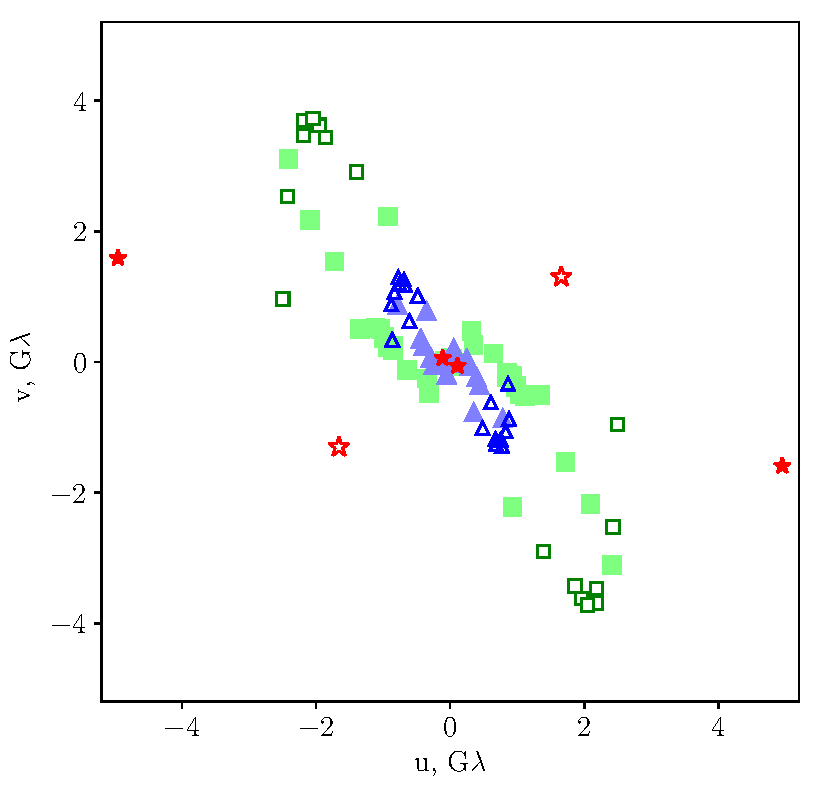
\includegraphics[width=0.7\textwidth]{0529_UV.pdf}
}
\caption{$(u, v)$ покрытие наблюдений B0529+483 на РадиоАстроне на \SI{1.7}{\GHz} (синие
треугольники), \SI{4.8}{\GHz} (зелёные треугольники) и \SI{22}{\GHz} (красные звёздочки).
Не закрашенные символы обозначают недетектирования.}
\label{fig:0529_uv}
\end{figure}

Наблюдения сильно кластеризованы в $(u, v)$-плоскости (см. рис.~\ref{fig:0529_uv}). Чтобы уменьшить
эффект этой кластеризации, мы вводим равномерные веса, вычисляя количество точек вокруг каждой точки
(включая себя) внутри круга радиуса $R$ в $(u, v)$-плоскости. Вес является обратным к этому числу.
Мы попробовали несколько значений $R$ и, наконец, приняли $R = \SI{150}{\mega\la}$: значения ниже
этого не влияют значительно на веса, в то время как значения выше \SI{600}{\mega\la} приводят к
вырождению между параметрами модели во время аппроксимации.


\subsubsection{Недетектирования на наземно-космических базах}

Из Таблицы 1 видно, что в ряде экспериментов не было обнаружено значимого сигнала на базах
КРТ-земля (наземные станции, с которых были обнаружены лепестки, подчеркнуты). В большинстве
случаев, когда не было обнаружений на наземно-космических базах, в том же эксперименте были
значимые детектирования на базах земля-земля. Это позволяет сделать вывод, что
оборудование на наземных станциях работало должным образом. Состояние оборудования на КРТ
контролируется с помощью подробной служебной телеметрии. Таким образом, во время наблюдений,
перечисленных в Таблице 1, не было выявлено сбоев. Кроме того, было много экспериментов со
значимыми детектированиями других источников, смежных по времени с необнаружениями для B0529+483.
Таким образом, эти необнаружения вряд ли были вызваны аппаратными проблемами, поэтому верхние
пределы амплитуд видимости в этих экспериментах могут быть извлечены из этих необнаружений.

Для определения подходящих верхних пределов мы использовали измеренные системные температуры
для расчета SEFD участвующих телескопов. В тех случаях, когда эта информация была
недоступна, мы использовали медианные значения SEFD. Основываясь на результатах экспериментов
обзора AGN (Ковалев и др., В процессе подготовки) с высоким SNR, мы находим времена
когерентного интегрирования для каждой полосы: \SI{400}{\second} на 1.7 и \SI{4.8}{\GHz} и
\SI{200}{\second} на \SI{22}{\GHz}. На этих временах интегрирования потери когерентности составляют
менее 2\,\%. Мы выбираем максимальный верхний предел $5\sigma$ для каждого эксперимента без
обнаружения и представляем их в таблице 4.

\subsection{Свойства B0529+483 на парсековых масштабах в случает отсутствия рассеяния}

\subsubsection{Нижние пределы и измерения по одной точки}

\begin{figure}[]
\centerfloat{
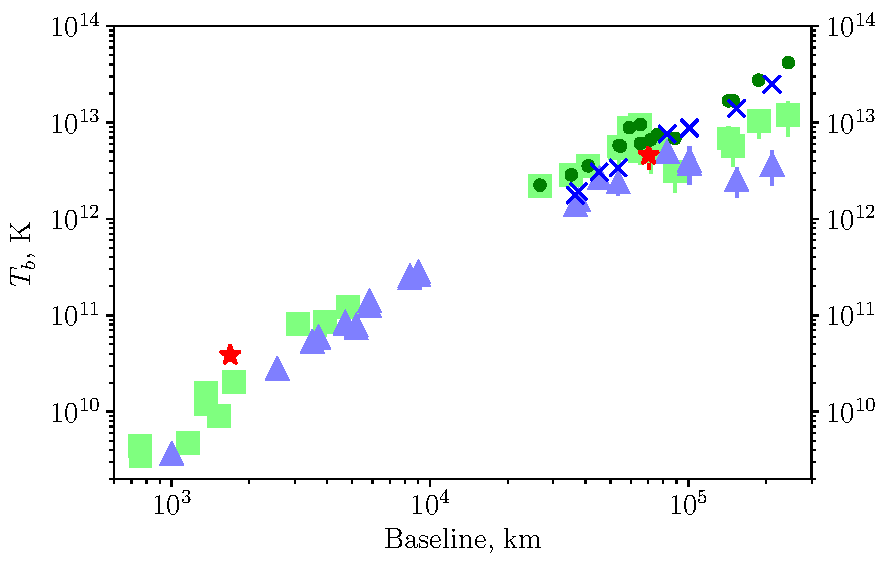
\includegraphics[width=0.7\textwidth]{0529_Tbmin.pdf}
}
\caption{Результаты измерений яркостной температуры B0529+483.}
\label{fig:0529_tb}
\end{figure}

В \cite{Lobanov_2015a} показано, что минимальная яркостная температура, $T_\text{b,min}$, может
быть оценена на основе одного измерения амплитуды видности $V_q$ на базовой линии $B$ для
предполагаемого кругового гауссова распределения интенсивности источника. Эти пределы яркостной
температуры для B0529+483 показаны на рис.~\ref{fig:0529_tb}. Космическая часть этого графика
охватывает проекции баз $B > \SI{e4}{\km}$. Установлено, что самые высокие нижние пределы
составляют \SI{5e12}{\kelvin} на \SI{1.7}{\GHz}, \SI{1.2e13}{\kelvin} на \SI{4.8}{\GHz} и
\SI{5e12}{\kelvin} на \SI{22}{\GHz}. Для нескольких примеров, представленных в \cite{Lobanov_2015a},
разница между яркостной температурой, полученной из моделирования, и нижним пределом для
разрешенного компонента находится в пределах 2 раз.


\begin{table}
\caption{Верхние пределы коррелированной плотности потока на наземно-космических базах для
экспериментов без детектирований.
Сокращения названий телескопов см. в таблице~\ref{tab:0529_exper}.}
\label{tab:0529_nodet}
\centering
\small
\begin{SingleSpace}
\begin{tabular}{llrrr}
\toprule
Код           & Базы & Проекция            & Позиционный & $5\sigma$, \\
эксперимента  & КРТ- & базы, \si{\giga\la} & угол, \si{\degree} & \si{\milli\jansky} \\
\midrule
 & & 4.8 GHz & & \\
\midrule
raks01ct & Gb &  1.15 & 154 &  13 \\
raks01cx & Ef &  1.37 & 151 &  19 \\
raks01da & Ys &  2.78 & 151 &  51 \\
raks01ea & Ef &  1.51 & 149 &  19 \\
raks01ex & Ev &  4.24 & 151 &  27 \\
raks08cx & Kz &  2.75 & 148 &  49 \\
raks08dc & Ef & 14.51 & 122 &  18 \\
raks08fv & Ys &  2.61 & 111 &  36 \\
raks08gq & Ys &  1.24 & 135 &  22 \\
\midrule
& & 1.7 GHz & & \\
\midrule
raes03kn & Wb &  1.35 & 142 &  49 \\
raes03lb & Bd &  0.87 & 136 &  38 \\
raks01ct & Gb &  1.12 & 154 &   7 \\
raks01cx & Gb &  1.36 & 150 &   7 \\
raks01da & Tr &  1.43 & 151 &  36 \\
raks01ea & Gb &  1.50 & 149 &   7 \\
raks08cx & Kl &  1.41 & 148 &  24 \\
raks08fv & Kl &  0.93 & 111 &  24 \\
raks08gq & Gb &  1.24 & 135 &   7 \\
\midrule
& & 22 GHz & & \\
\midrule
raes03dk & Gb &  6.93 & 112 &  61 \\
raes03hk & Gb & 15.56 & 139 &  61 \\
raes03hm & Gb & 17.58 & 143 &  61 \\
raes03ia & Ef & 13.82 & 136 & 105 \\
raes03ks & Ys &  2.11 &  52 & 156 \\
raks08dc & Gb & 14.83 & 121 &  61 \\
\bottomrule
\end{tabular}
\end{SingleSpace}
\end{table}

Недетекты, представленные в Таблице~\ref{tab:0529_nodet}, охватывают более длительный интервал
времени, чем наши
успешные детектирования. Нижний предел яркостной температуры, полученный из необнаружений,
охватывает диапазон от \num{3.5e12} до \SI{2.3e13}{\kelvin} на \SI{1.7}{\GHz}, от \num{1.8e12} до
\SI{1.9e13}{\kelvin} на \SI{4.8}{\GHz} и от \num{0.8e12} до \SI{2.4e13}{\kelvin} на \SI{22}{\GHz}.
Это может отражать переменность B0529+483.

Можно также оценить яркостную температуру компактной детали источника, предполагая, что для
наиболее компактного компонента используется модель одной круговой гауссианы, считая среднее
значение амплитуд видностей на наземных базах в качестве амплитуды гауссианы и определяя её
ширину из единичного измерения видности на наземно-космической базе. Результаты таких оценок также
показаны на рис. 5 с повышением яркостной температуры до \SI{3e13}{\kelvin} на частоте
\SI{1.7}{\GHz} и \SI{5e13}{\kelvin} на частоте \SI{4.8}{\GHz}.

Обратите внимание, что оба эти метода могут переоценить яркостную температуру источника, при
наличии рефракционной субструктуры от рассеяния \cite{Johnson_2015,Johnson_2016}.

\subsubsection{Гауссовы модели}

В этом разделе мы строим более сложную модель, которая нацелена на подгонку ко всем данным
видности. Мы используем метод взвешенных наименьших квадратов для определения параметров модели,
которые представлены в таблице~\ref{tab:0529_fit}.

\begin{figure}[]
\centerfloat{
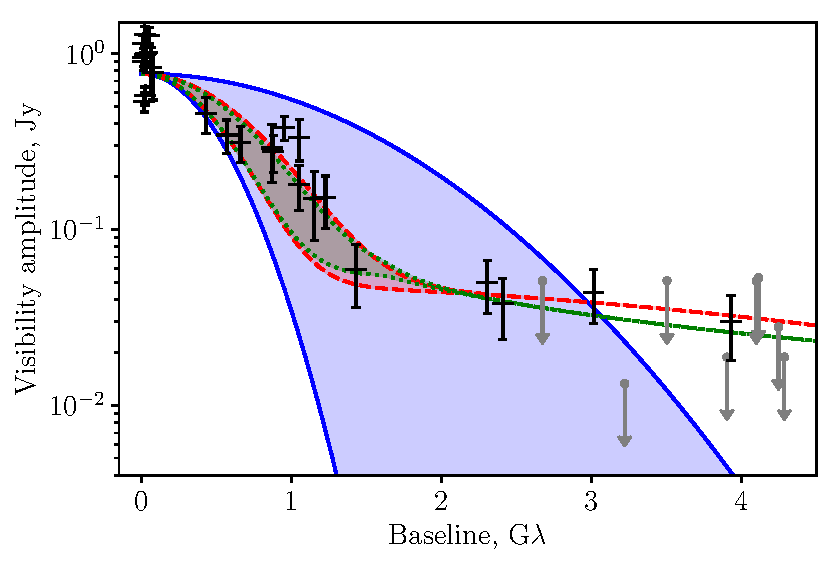
\includegraphics[width=0.49\textwidth]{0529_1dplotC.pdf}
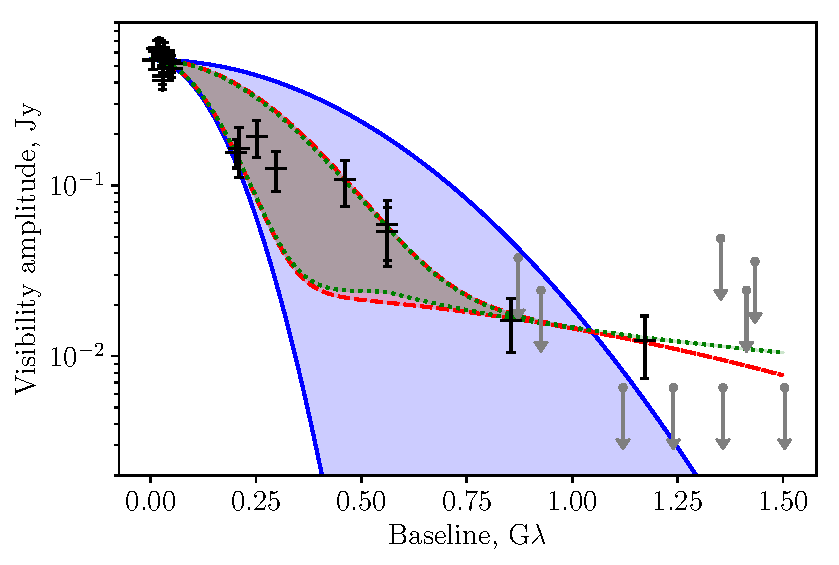
\includegraphics[width=0.49\textwidth]{0529_1dplotL.pdf}
}
\caption{Амплитуда видности как функция длины базы на частоте \SI{4.8}{\GHz} (слева) и
\SI{1.7}{\GHz} (справа). Столбики ошибок представляют данные РадиоАстрона, синюю область между
сплошными линиями~"--- одну эллиптическую гауссовскую модель, красную область между пунктирными
линиями~"--- двойную гауссову модель, зеленую область между пунктирными линиями~"--- модель с
рефракционной субструктурой. Границы заштрихованных областей соответствуют малой и большой осям
модели, сами области охватывают значения амплитуды видности для различных позиционных углов.
Верхние пределы, показанные точками с ошибками, представляют результаты из
таблицы~\ref{tab:0529_nodet}.}
\label{fig:0529_1dplot}
\end{figure}

Мы начнем с модели с одной эллиптической гауссианой, которая в таблице 5 называется
<<одиночная Гауссиана>>. Она имеет довольно большое значение $\chi^2_\text{reduced}$, которое мы
интерпретируем как результат простоты модели: из рисунка~\ref{fig:0529_1dplot} можно видеть, что
точки на самых длинных базах плохо описываются этой моделью.

Мы добавили второй круглый гауссовский компонент к этой модели и называли его <<двойная
Гауссиана>>. В этом случае $\chi^2_\text{reduced}$ намного более разумно; отличие от 1.0 на
\SI{4.8}{\GHz} обусловлено особенностью на $\sim$\SI{1}{\giga\la} на рис.~\ref{fig:0529_1dplot},
которая не очень хорошо описывается моделью. Эта особенность представлена только двумя точками из
двух экспериментов (raes03hv, raes03kg). Отклонения точек данных от модели составляют 2.6 и
1.2$\sigma$. Это может быть результатом переменности источника, поскольку два эксперимента
предшествуют, но близки к максимуму вариаций общей плотности потока на \SI{15}{\GHz} на рис. 3.

Из рис.~\ref{fig:0529_uv} видно, что распределение наших измерений на $(u, v)$-плоскости сильно
вытянуто (как для детектирований, так и для недетектирований). Из таблицы 5 видно, что малые полуоси
в реальной плоскости более крупных компонентов в наших моделях примерно совпадают с направлением
этого удлинения. Это может быть случайностью. Во-первых, ориентация эллиптических компонентов
определяется точками на базах $<$\SI{0.5}{\giga\la} на \SI{1.7}{\GHz} и $<$\SI{1.5}{\giga\la} на
\SI{4.8}{\GHz}. На этих масштабах на рис. 1 точки распределены более равномерно по позиционным
углам. Во-вторых, ориентация компонентов нашей модели совпадает с ориентацией ядра на наземных РСДБ
картах, поэтому мы считаем, что позиционные углы, приведенные в таблице~\ref{tab:0529_fit}, не
являются артефактами моделирования.

В таблицах 1 и 2 перечислены несколько экспериментов на частоте \SI{4.8}{\GHz}, в которых сигнал
был обнаружен на базах линиях, образующих треугольник (raes03en, raes03eo и raes03hv). Это
позволяет нам анализировать замыкания фазы, которые в принципе несут значительную информацию о
распределении яркости в источнике, и в то же время, при скромных предположениях, не содержат
систематического фазового шума \cite{VLBIbook}. Отметим, однако, что плохое $(u, v)$-покрытие
и высокое вырождение замыкающих треугольников (базы земля-КРТ почти равны и намного
длиннее, чем база земля-земля), значительно снижают эффективность метода
\cite{Linfield_1986,Marti_Vidal_2008}.

Тем не менее, мы измерили замкнутые фазы и использовали их в процедуре подгонки. Соотношение
сигнал/шум в обсуждаемых экспериментах низкое, и только в одном из этих экспериментов, raes03en,
замыкание фазы оказывается выше порога обнаружения. Мы использовали значения замыкания фазы из всех
трех экспериментов, чтобы получить проверку согласованности нашей модели распределения яркости на
основе анализа амплитуд видности, представленных выше. В частности, мы варьировали расстояние
между компонентами в модели <<двойная Гауссиана>>. Качественно модели замыкания фаз согласуются с
амплитудным моделированием. Из-за отсутствия данных фазы этот результат сильно зависит от модели, и
измеренная замкнутая фаза может быть объяснена без введения смещения между компонентами, например,
путем добавления небольшой асимметрии к наибольшему компоненту модели. Мы отмечаем, что к этому
результату следует относиться с осторожностью из-за ограниченности имеющихся данных и низких
значений SNR. В частности, хотя качественно модель замыкания фазы, по-видимому, допускает решения,
основанные на амплитуде, две вылетевшие точки в районе $\sim$\SI{1}{\giga\la} на
рис.~\ref{fig:0529_1dplot} (слева) плохо согласуются.

Наличие сигнала на длинных базах космос-земля также можно объяснить влиянием субструктуры,
созданной рефракционным рассеянием, на неоднородности межзвездной среды \cite{Johnson_2015}. Мы
обсуждаем эту возможность в разделе 4. Альтернативно, она может возникнуть из-за внутренней
мелкомасштабной структуры источника \cite{Gomez_2016, Kovalev_2016}. Если детектирования на
самых длинных базах отражает внутренние параметры ядра, яркостная температура ядра составляет
величину \SI{0.4e13}{\kelvin} на \SI{1.7}{\GHz}, \SI{1.7e13}{\kelvin} на \SI{4.8}{\GHz} и
\SI{1e13}{\kelvin} на \SI{22}{\GHz}.

Верхние пределы и детектирования на больших проекциях базы, представленные в
таблице~\ref{tab:0529_nodet} и на рисунке~\ref{fig:0529_1dplot}, показывают значительный разброс. Из
рисунка~\ref{fig:0529_uv} видно, что векторы проекций базовой линии для недетектирований близки к
таковым для детектирований, поэтому разброс не может быть объяснено асимметрией источника. Это может
быть объяснено переменностью плотности потока ядра или его структуры: недетектирования охватывают 2
года наблюдений, в то время как успешные детектирования только 5 месяцев. В то время как изменение
видимого углового размера источника из-за физического изменения линейного размера источника не может
быть исключено, его амплитуда ограничена принципом причинности (линейное изменение размера не может
превышать расстояние, которое проходит свет за характерное время переменности). В следующем анализе
мы не приписываем недетектирования структурным изменениям (то есть увеличение линейного размера
компактного компонента, приводящее к его разрешению). Мы также можем недооценивать чувствительность
детектирования в некоторых случаях, особенно если погодные условия были плохими. Из-за этого
большого разброса мы не используем верхние пределы для дальнейшего ограничения моделей,
представленных здесь.

В Таблице~\ref{tab:0529_nodet} есть один момент, который заслуживает отдельного обсуждения: в
эксперименте \texttt{raes03ks} не было детектирования на частоте 22~ГГц на относительно небольших
проекциях базы, \SI{2.1}{\giga\la}. В этом эксперименте Yebes был единственным наземным
радиотелескопом, поэтому мы не можем быть уверены, что это недетектирование не вызвано неопознанным
отказом оборудования. С другой стороны, в тот же день Yebes дал лепестки на \SI{4.8}{\GHz} в другом
эксперименте. Если мы считаем фактическое отсутствие детектирования на \SI{22}{\GHz} реальным, это
не согласуется с круговой гауссовой моделью для данных \SI{22}{\GHz}, представленной в таблице 5.
Недетектирование расположено почти точно на самой большой полуоси в плоскости изображения компоненты
модели <<двойная Гауссиана>> на частотах 4.8 и \SI{1.6}{\GHz} в таблице 5 (см. также пустые красные
звезды на рис.~\ref{fig:0529_uv}). Если мы подгоним эллиптическую модель Гаусса к данным
\SI{22}{\GHz} с учетом этого отсутствия детектирования, мы получим размеры FWHM $0.08 \times
0.03$\,\si{\mas} и $T_\text{b} = \SI{0.5e13}{\kelvin}$. Отличие от значений в Таблице 5 не влияет на
наши результаты, поэтому мы также не рассматриваем эту обновленную модель, которая включает
(неопределенное) отсутствие обнаружения.

\begin{table}
\caption{The fit parameters for the measured amplitudes. See description of the models in text. The
errors are one standard deviation. The angular sizes, $\theta_a$ and $\theta_b$, are FWHMs. Position
Angles are given for the largest semi-axis at the real plane. When an error is not given this means
that the parameter was fixed.}
\label{tab:0529_fit}
\centering
\tiny
\begin{SingleSpace}
\begin{tabular}{lllllllr}
\toprule
Model                     & $S_0$,   & $\theta_a$, & $\theta_b$, & P.A., & $C$, & $T_\text{b}$,
& $\chi^2_\text{reduced}$\\
                          & \si{\milli\jansky} & \si{\mas} & \si{\mas} & \si{\degree} &
\si{\milli\jansky}  & $10^{13}$\,K & \\
\midrule
4.8 GHz & & & & & & & \\
Single Gaussian           & $770 \pm 30$ & $0.19 \pm 0.01$  & $0.06 \pm 0.001$ & $36 \pm 1$  & -- &
$0.71 \pm 0.08$& 6.0 \\
Double Gaussian, comp.\ 1 & $720 \pm 40$ & $0.18 \pm 0.05$  & $0.13 \pm 0.038$ & $47 \pm 38$ & -- &
$0.34 \pm 0.20$& 3.2 \\
Double Gaussian, comp.\ 2 & $ 48 \pm  6$ & $0.018\pm 0.015$ & $0.018\pm 0.015$ & --          & -- &
$1.7\pm0.8$ & \\
Gaussian + Substructure   & $700 \pm 30$ & $0.19 \pm 0.05$  & $0.14 \pm 0.040$ & $51 \pm 57$ & $60
\pm 11$ & $0.30 \pm 0.18$& 3.1 \\
\midrule
1.7 GHz & & & & & & & \\
Single Gaussian           & $550 \pm 20$ & $0.64 \pm 0.05$ & $0.20 \pm 0.005$ & $37 \pm 1$ & -- &
$0.41 \pm 0.05$& 4.5 \\
Double Gaussian, comp.\ 1 & $520 \pm 20$ & $0.64 \pm 0.09$ & $0.31 \pm 0.028$ & $47 \pm 5$ & -- &
$0.25 \pm 0.06$& 1.2 \\
Double Gaussian, comp.\ 2 & $ 24 \pm  4$ & $0.08\pm0.06$   & $0.08 \pm 0.06$  & --         & -- &
$0.4\pm0.3$ \\
Gaussian + Substructure   & $520 \pm 20$ & $0.64 \pm 0.09$ & $0.32 \pm 0.027$ & $47 \pm 5$ & $23 \pm
6$ & $0.24 \pm 0.06$& 1.2 \\
%Broadening+Substructure & $0.5\pm0.1$ & 0.9 & 0.9 & -- & $0.011\pm0.09$ & $0.007\pm0.002$ & 1.0 \\
%NE2001+Substructure & $0.6\pm0.1$ & 1.25 & 1.25 & -- & 0.006 & $0.004\pm0.001$ & 1.5 \\
\midrule
22 GHz & & & & & & & \\
Gaussian (circular)       & 2200              & 0.034 & 0.034 & -- & -- & 1.0 & -- \\
\bottomrule
\end{tabular}
\end{SingleSpace}
\end{table}

\subsection{Проявления рефракционного рассеяния}

\subsection{Обсуждение}

Данные указывают на наличие по меньшей мере двух компонентов в каждом из диапазонов 1.7 и
\SI{4.8}{\GHz} в структуре B0529+483 на наземно-космических базах интерферометра, параметры которых
приведены в таблице~\ref{tab:0529_fit}. Мы предполагаем, что более крупные компоненты модели на
двух частотах представляют та же физическая структура~"--- ядро квазара. Это подтверждается
примерным совпадением размеров и плотностей потоков ядра, измеренных наземным РСДБ (рис. 3 и
8) и RadioAstron (таблица~\ref{tab:0529_fit}). Если это предположение верно, больший компонент
модели <<двойного гаусса>> в таблице~\ref{tab:0529_fit} имеет масштабирование по частоте с
$\nu^{-0.9}$. Это близко к внутренним свойствам ядра, связанным с синхротронным самопоглощением,
ожидаемым по модели \cite{Blandford_Konigl_1979} и измеренным для блазаров \cite{Kutkin_2014}.
Масштабирование размера $\propto\nu^{-1}$ также согласуется с нашими наземными РСДБ данными. Для
малой компоненты масштабирование не может быть точно определено и составляет
$\propto\nu^{-1.2\pm2}$.

Поскольку квазар находится вблизи плоскости Галактики, можно ожидать наличия рефракционного
рассеяния. Мы рассмотрели предположение о том, что большой компонент представляет собой угловое
расширенное изображение источника, в то время как малый компонент представляет собой рефракционную
субструктуру. Эта гипотеза опровергается масштабированием наблюдаемого углового уширения в этом
случае, что сильно не согласуется с ожидаемым законом рассеяния. Отметим, что
\cite{Pushkarev_Kovalev_2015} проанализировали большой набор внегалактических источников в диапазоне
галактических широт. Они обнаружили, что размеры ядер внегалактических радиоисточников вдали от
плоскости Галактики показывают масштабирование $\nu^{-1}$, в то время как около 1/3 AGN вблизи
плоскости Галактики демонстрируют масштабирование, соответствующее ожидаемому для рассеяния. Мы
также исключаем рассеяние, предсказанное по модели NE2001 \cite{Cordes_2002}, поскольку большие
разрешенные компоненты B0529+483 имеют размеры меньше, чем предсказывает модель.

Мы заключаем, что наши результаты могут быть объяснены любой из следующих двух гипотез. Первая
заключается в том, что в наблюдениях B0529+483 с RadioAstron отсутствуют эффекты рефракционного
рассеяния. Это означает, что даже вблизи плоскости Галактики разрешение в десятки микродугсекунд
может быть достигнуто на относительно низких частотах 1.7--5~ГГц. Вторая~"--- малая ось большого
компонента на частоте \SI{1.7}{\GHz} уширена рассеиванием. В этом случае два детектирования на
самых длинных базах на \SI{1.7}{\GHz} представляют рефракционную субструктуру. На частоте
\SI{4.8}{\GHz} шкала углового уширения должна составлять \SI{0.04}{\mas}. Предположение о том, что
малый компонент источника на частоте \SI{4.8}{\GHz} фактически представляет собой угловое
расширенное ядро, согласуется с данными.

Если рассеяние влияет на малый компонент на частоте \SI{4.8}{\GHz}, он также может подвергаться
межзвездной сцинтилляции. В этом случае недетекты на рисунке~\ref{fig:0529_1dplot} могут быть
интерпретированы как результат этих мерцаний: компонент был обнаружен только тогда, когда он был
рассеян. В этом случае амплитуда и яркостная температура малого компонента могут быть
уменьшены в 2 раза. Малая амплитуда этого (\SI{0.02}{\jansky}), по сравнению с большим компонентом
(\SI{0.7}{\jansky}), к сожалению, не даёт обнаружить этих сцинтилляций с помощью наблюдений
за однодневной изменчивостью на одиночных телескопах.

В обеих этих гипотезах малый компонент на частоте \SI{4.8}{\GHz} не создается рефракционной
субструктурой. Это означает, что нижний предел яркостной температуры для B0529+483 на
\SI{4.8}{\GHz} составляет \SI{1e13}{\kelvin} (Таблица 7). Это согласуется также с оценкой яркостной
температуры на частоте \SI{22}{\GHz}, которая не зависит от рассеяния, и равна \SI{e13}{\kelvin},
см. таблицу~\ref{tab:0529_fit}. В \cite{Lister_2016} измерили максимальную кажущуюся скорость
струи на парсековых масштабах этого квазара, равную $v_\text{app}=19.8\pm3.0\,c$. В случае
равновесия между энергией частиц и магнитного поля, предел составляет \SI{e10.5}{\kelvin}, поэтому
необходимо нереально высокое доплеровское усиление $\delta > 300$. Доминирование энергии частиц
над магнитной энергией во многих АЯГ также подтверждается \cite{Nokhrina_2017}.

С другой стороны, следуя \cite{Readhead_1994}, мы можем оценить временную шкалу потери энергии
электронов по повышенным значениям яркостной температуры и частоты наблюдения. Если доплеровское
усиление $\delta \approx 1$, временные масштабы намного меньше \SI{1}{\second} на обеих частотах.
Взяв допплеровское усиление $\delta\approx v_\text{app}/c$, мы находим, что временные шкалы
составляют $\sim$100 лет на \SI{4.8}{\GHz} и около 1 года на \SI{2}{\GHz}. Время указано в системе
отсчёта наблюдателя. Обе эти временные шкалы длиннее, чем временные масштабы наших наблюдений
высокой яркостной температуры; таким образом, наши результаты для B0529+483 не оспаривают обратный
Комптоновский предел. Сравнение потока радио и $\gamma$-квантов на рис. 4 не показывает каких-либо
свидетельств сильного увеличения потока $\gamma$-квантов в период детектирования лепестков на
РадиоАстроне, которые могли бы накачивать энергию электронов и повышать яркостную температуру выше
обратного Комптоновского предела (см., например, \cite{Readhead_1994,Kovalev_2016}).

\subsection{Заключение}

РадиоАстрон продетектировал квазар B0529+483 на частотах 1.7, 4.8 и \SI{22}{\GHz} на проекциях базы
до 240\,000\,км. Анализ амплитуды видности в зависимости от проекции базы
демонстрирует наличие по крайней мере двух компонентов, один из которых разрешен, а другой~"---
нет. Мы находим, что данные согласуются с двумя возможностями: либо РадиоАстрон не детектирует
субструктуру рефракционного рассеяния для этого источника с низкой галактической широтой, либо
рассеяние является значительным только на \SI{18}{\cm}. В любом случае, рассеяние для этого
конкретного квазара оказалось намного слабее, чем предсказывалось моделью NE2001
\cite{Cordes_2002}. Яркостная температура ядра B0529+483 в системе отсчёта источника превышает
\SI{e13}{\kelvin} при 4.8 и \SI{22}{\GHz}. Это указывает на сильное доминирование плотности энергии
частиц над плотностью энергии магнитного поля в ядрах квазара; в противном случае требуется
чрезвычайно сильное доплеровское усиление, $\delta > 300$. Для обратного комптоновского предела
$T_\text{b} \sim \SI{e11.5}{\kelvin}$ требуется $\delta \sim \text{20--30}$, что не является
необоснованным.
